\documentclass[]{thesis}

\DeclareAcronym{SAT}{
  short=SAT,
  long=boolean satisfiability problem,
}

\DeclareAcronym{DL}{
  short=DL,
  long=deep learning,
}

\DeclareAcronym{ML}{
  short=ML,
  long=machine learning,
}

\DeclareAcronym{GNN}{
  short=GNN,
  long=graph neural network,
}

\DeclareAcronym{MUS}{
  short=MUS,
  long=minimal unsatisfiable subset,
  short-plural=es,
}

\DeclareAcronym{PGE}{
  short=PGExplainer,
  long=parameterized explainer for graph neural networks,
}

\DeclareAcronym{MLP}{
  short=MLP,
  long=multilayer perceptron,
}

\DeclareAcronym{GCN}{
  short=GCN,
  long=graph convolutional network,
}

\DeclareAcronym{CNN}{
  short=CNN,
  long=convolutional neural network,
}

\DeclareAcronym{MPNN}{
  short=MPNN,
  long=message passing neural network,
}

\DeclareAcronym{CNF}{
  short=CNF,
  long=conjunctive normal form,
}

\DeclareAcronym{LCG}{
  short=LCG,
  long=literal-clause graph,
}

\DeclareAcronym{ROC-AUC}{
  short=ROC-AUC,
  alt = AUROC,
  long=area under the receiver operating characteristic curve,
}

\DeclareAcronym{ROC}{
  short=ROC,
  long=receiver operating characteristic,
}

\DeclareAcronym{AUC}{
  short=AUC,
  long=area under the curve,
}

\DeclareAcronym{GT}{
  short=GT,
  long=ground truth,
}

\DeclareAcronym{BA}{
  short=BA,
  long=Barabási-Albert,
}

\DeclareAcronym{TM}{
  short=TM,
  long=target model,
}


\begin{document}

    \definecolor{codegreen}{rgb}{0,0.6,0}
    \definecolor{codegray}{rgb}{0.5,0.5,0.5}
    \definecolor{codepurple}{rgb}{0.58,0,0.82}
    \definecolor{backcolour}{rgb}{0.95,0.95,0.92}


    \lstdefinestyle{mystyle}{
        backgroundcolor=\color{backcolour},   
        commentstyle=\color{codegreen},
        keywordstyle=\color{magenta},
        numberstyle=\tiny\color{codegray},
        stringstyle=\color{codepurple},
        basicstyle=\ttfamily\footnotesize,
        breakatwhitespace=false,         
        breaklines=true,                 
        captionpos=b,                    
        keepspaces=true,                 
        numbers=left,                    
        numbersep=5pt,                  
        showspaces=false,                
        showstringspaces=false,
        showtabs=false,                  
        tabsize=2
    }

    \lstset{style=mystyle}

    \pagenumbering{roman}
    \begin{titlepage}
    \begin{center}
        \begin{minipage}[t]{\textwidth}
            \raggedleft
            
\includegraphics[width=0.35\textwidth]{img/tud-logo.pdf}
        \end{minipage}
    
        \vspace{3cm}
            
        \Huge
        \textbf{Providing Bipartite GNN Explanations with PGExplainer}
            
        \vspace{1.5cm}
            
        \LARGE
        \textbf{Tristan Marten Lewin Schulz}
            
        \vspace{1.5cm}
          
        \Large
        Bachelor of Science\\
        May 19, 2025\\
    \end{center}

    \vfill

    \noindent
    \begin{minipage}[t]{0.5\textwidth}
        \raggedright
        \Large
        Supervisors:\\
        Prof. Dr. Stefan Harmeling\\
        Lukas Schneider\\
    \end{minipage}
    \hfill
    \begin{minipage}[t]{0.5\textwidth}
        \raggedleft
        \Large
        Artificial Intelligence (VIII)\\
        Department of Computer Science\\
        TU Dortmund University\\
    \end{minipage}
\end{titlepage}

    \cleardoublepage

    \phantomsection
    \addcontentsline{toc}{chapter}{Abstract}
    \chapter*{Abstract}

%Context/Background: Why is this topic and this research important?
%Objective: What questions are you trying to answer in your research?
%Methods/Design: What are the basic details of your research? In general, how did you go %about answering the research questions? 
%Results: What answers did you find? Were there any other observations?
%Conclusion/Takeaways: Were your results expected? Is more research needed?


The recent advances in \ac{DL} have lead to \ac{ML} approaches for solving the \ac{SAT}, commonly represented as a bipartite graph problem, with NeuroSAT being a prominent example utilizing a \ac{GNN}. However, models like these often suffer from a lack of natural proofs or explanations of their predictions, hindering the trustworthiness as well as practical cross-domain applicability. In this work, we explore a method that provides instance explanations with a global view of the GNN, thus seeking to generally explain a model's predictions. We reimplement the \ac{PGE} using PyTorch Geometric, testing its generalizability in the inductive setting and extending it to the domain of NeuroSAT.

While our replication showed that the framework succeeds in generating inductive explanations for structurally similar node instances, it struggles with generalizing these across different node instances of a motif. At the same time, general explanations for graph instances showed promising results. To apply the PGExplainer on NeuroSAT and generate explanations for SAT instances, we interpret unsatisfiable SAT instances using \acp{MUS} - small unsatisfiable cores - as \ac{GT}. Though we were unable to generate favorable explanations that consistently align with these, our findings indicate potential measures for future work and highlight the need for more robust and generalizable methods. 
    \cleardoublepage

    % USE THIS TO HIDE SUBSECTIONS IN TOC
    \setcounter{tocdepth}{1}
    \tableofcontents
    \cleardoublepage

    \cleardoublepage
    \phantomsection
    \addcontentsline{toc}{chapter}{List of Figures}
    \listoffigures

    \cleardoublepage
    \phantomsection
    \addcontentsline{toc}{chapter}{List of Tables}
    \listoftables

    \cleardoublepage
    \phantomsection
    \addcontentsline{toc}{chapter}{List of Acronyms}
    \acsetup{list/name = {List of Acronyms}}
    \printacronyms

    \cleardoublepage
    \pagenumbering{arabic}
    \let\cleardoublepage\clearpage
    \chapter{Introduction}
\label{ch:Introduction}

SAT motivation: Advancements in deep learning SAT solving, e.g. NeuroSAT. Need for evaluation of these models! use of GNN explainers, since SAT can be reduced to graph domain. GOAL: Application of PGExplainer on NeruoSAT to generate explanations. Explanations need gt to be evaluated on accuracy. Use concepts like unsat cores as gt and compare to explanations provided by PGExplainer to see whether NeuroSAT explanations align with "human-observable" principles.
Concrete: Graph task: Prediction of UNSAT and unsat cores as gt. Node task: Difficult with NeuroSAT?\bigskip

Therefore explanation and replication of PGExplainer. After successful replication, application on NeuroSAT. \bigskip

PGExplainer claims to be model-agnostic - Works for any GNN. Additionally, able to generate explanations in an inductive setting, which is what we want to do.\bigskip

Since our goal is application on a bipartite problem, reimplementation of PGExplainer that changes architecture of target GNN to a PyG layer that works on bipartite graphs and also allows passing of edge weights (required for PGE).\bigskip

Pytorch reimplemenations already exist, eg. Replication study RE-PGE that focuses on orginal code to replicate results. We follow paper as close as possible, and also conduct the code to try different settings/hyperparameters for our changed GNN - OUR FOCUS: Evaluate whether PGExplainer still applicable for our slightly changed GNN model!\bigskip

Therefore, use PGExplainer and Repliaction paper as baselines to compare our results (INDUCTIVE SETTING!) \bigskip

Lastly, apply PGExplainer NeuroSAT, a solver for bipartite graph problem SAT inductively
    \chapter{Theoretical Background}
\label{ch:Background}
In this chapter we define the necessary background for understanding PGExplainer as well as the follow-up work regarding its application on the Boolean Satisfiability Problem (SAT). We start by giving an introduction to deep learning in Section \ref{sec:deep_learning}, including a specific architecture and regularization techniques. In Section \ref{sec:graph_theory} we define the necessary graph theory, including bipartite graphs and random graphs. To understand the motivation behind the objective of PGExplainer we outline the relevant concepts of information theory, namely entropy, cross-entropy and mutual information, in Section \ref{sec:information_theory}. Since the explainer model operates on Graph Neural networks, we introduce the historically relevant GNN model by Scarselli et al. \cite{4700287} in Section \ref{sec:gnns}, as well as two succeeding models. After introducing the most relevant concepts, in Section \ref{sec:gnn_explainability} we briefly discuss the field of explainability in graph neural networks to motivate the selection of this approach for our work. Lastly, in Section \ref{sec:SAT} we describe the boolean satisfiability problem that motivates this work.

\section{Deep learning}
\label{sec:deep_learning}
TODO: Generally more examples, sources etc., to convey broad knowledge in the field

In this chapter we introduce Deep Learning (DL) in the context of Machine Learning (ML) and their concepts required for this work. The definitions in this chapter loosely follow Goodfellow et al. \cite{Goodfellow-et-al-2016}.

ML algorithms generally learn to perform certain tasks from data that can broadly be divided into supervised and unsupervised learning. In this work, we focus on supervised learning, meaning that the algorithm learns from a dataset containing both features and labels or targets that the algorithm is supposed to predict. In other words, the algorithm learns from a training set of input examples, defined as vectors $\mathbf{x} \in \mathbb{R}^n$, with entries $x_i$ denoting features, and output examples $\mathbf{y}$, whose shape depends on the task at hand. Its goal is to be able to associate unseen inputs from a set of test data, coming from the same distribution as the training data, with some target output. This process estimates the generalization error of the learner after the training is complete. 
Common supervised ML tasks include classification, assigning an input to one of $k$ categories, and regression, where the program shall predict a numeric value given some input. 
TODO: WHAT IS A MODEL?

%Deep learning entails adding more layers and units to the model used in our algorithm to allow for representations of functions with increasing complexity.

DL entails expanding the size of the model used in our algorithm to allow for representations of functions with increasing complexity. This enables many human-solvable tasks that consist of mapping an input vector to an output vector to be performed with DL, given sufficiently large models and datasets. Most notably, Krizhevsky et al. \cite{krizhevsky2012imagenet} achieved record-breaking results by using a large, deep convolutional network for image classification.

TODO: LAYER AND PARAMETER NOT YET DEFINED HERE
However, increasing the size of a model comes with new challenges. Since models become more complex with increasing number of layers, subnetworks and parameters, they are commonly treated as a "black box", as it is difficult to explain their decision-making process \cite{noor2024survey}. Thus, the need for methods that can explain and interpret such models arises. Furthermore, the increasing number of parameters directly raises the computational complexity, resulting in longer training times and higher hardware requirements. This may also impose limitations when deploying the model on low-resourced end-devices.

TODO: Formally define objective? What exactly does it do?
In many cases DL involves optimizing an objective function, usually by minimizing $f(x)$, that guides the model. This objective function is also referred to as loss function in the context of minimization. %We denote $x^*=\text{arg min} f(x)$.
To minimize a function $y = f(x)$, where $y,x \in \mathbb{R}$, we make use of the derivative $f'(x)$ that tells us how to change $x$ in order to get an improvement in $y$. We can reduce $f(x)$ by moving $x$ in the direction opposite of the sign of its derivative, since $f(x-\epsilon \text{ sign}(f'(x))) < f(x)$ for small enough $\epsilon$. Since we usually want to minimize a function with multiple inputs, we let $\mathbf{x} \in \mathbb{R}^n$ be a vector with $n$ elements. The partial derivative $\frac{\partial}{\partial x_i}f(\mathbf{x})$ is utilized, telling us how $f$ changes when only $x_i$ increases at point $\mathbf{x}$. To generalize this to a vector, the gradient $\nabla_xf(\mathbf{x})$ of $f$ is defined as the vector containing all partial derivatives. The aforementioned technique used to minimize a function is hence called gradient descent (see Cauchy\cite{cauchy1847methode}).

Ultimately, a DL algorithm typically consists of the following components: a dataset, an objective function, an optimization procedure like gradient descent, and a model. %5.10

We generally control an ML algorithm by tuning the hyperparameters, which are settings used to control its behavior that are not adapted by the algorithm itself. Settings that are difficult to optimize may be selected as hyperparameters. Common examples are the number of epochs - the iterations over the full training data - and the learning rate, that controls how much the model adjusts the weights at each step. An additional goal is finding the combination of hyperparameter settings that leads to the best performance of our model. This may also be automated with searching or learning algorithms.

To tune the hyperparameters we need a validation set of data that is not directly observed by the training algorithm, since the test data may not be used for making decisions about our model. This set estimates the generalization error during training. The training data is therefore commonly split into two disjoint sets, the training set and the validation set, with a standard split being $80/20$.

A traditional approach for tuning hyperparameters is the grid search, as described in Liashchynskyi et al. \cite{liashchynskyi2019grid}. This method involves defining a subspace of the complete hyperparameter space and searching for the best-performing training algorithm across all possible combinations within that subspace.

\subsection{Multilayer Perceptron}
TODO: consisting of multiple layers of hidden units and nonlinear activation functions
A classical DL model is the multilayer perceptron (MLP), first proposed by Rosenblatt \cite{rosenblatt1958perceptron}, with the general goal of approximating a function $f^*$. In the case of classification we could define a function $y = f^*(x)$ that maps an input $x$ to a label $y$. The MLP then defines the mapping $y = f(x;\boldsymbol{\theta})$ and learns the value of the parameters $\boldsymbol{\theta}$ that best approximate the function. At the start of the training these parameters are initialized randomly or by a smart initialization strategy, like the Glorot/Xavier initialization \cite{glorot2010understanding}. 

These models are also referred to as feedforward neural networks, as they process information from $x$, through the intermediate computations that define $f$, to the output $y$ without feedback connections that would feed outputs back to itself. The name network is derived from their representation as a composition of multiple different functions, that are described by a directed acyclic graph. An example network is $f(x) = f^{(3)}(f^{(2)}(f^{(1)}(x)))$ that consists of input layer $f^{(1)}$, hidden layer $f^{(2)}$ and output layer $f^{(3)}$. The length of this chain of functions defines the depth of a model, coining the term "deep learning". 

The approximation is achieved by training our network with training data, that consists of approximated examples of $f^*(x)$ at different points in the training and labels $y\approx f^*(x)$. These training examples dictate the output layer to generate a value close to $y$ for each input $x$, or to produce a higher-level representation that can be used for subsequent tasks. The learning algorithm then learns to utilize the other hidden layers, without specified behaviors, to achieve the best approximation. It is to note that the hidden layers are vector-valued with each vector element, referred to as unit, loosely taking the role of a neuron in neuroscience. This comparison is a common analogy to convey the idea of information processing. Models are therefore also referred to as neural networks.

%We use non-linear activation functions in layers to describe features and keep the model from learning a strictly linear transformation of its inputs. Result for a layer is vector of hidden units $h=g(W^Tx+b)$, where $W$ contains the weights of a linear transformation and b the biases. x is the input vector. $g$ is the activation function that is usually applied element-wise, such as ReLU or Sigmoid.

An input or intermediate layer for our model could be defined as:
\begin{equation}
    f^{(i)}(\mathbf{x}; \mathbf{W},\mathbf{c})=\mathbf{W}^\top\mathbf{x}+\mathbf{c},
\end{equation}
where $\mathbf{W} \in \mathbb{R}^{m\times n}$ contains the weight matrix for $m$ units with $n$ features and $\mathbf{c}\in \mathbb{R}^m$ is a vector of bias terms.
To keep the model from strictly learning a linear function of its inputs we can calculate the vector of hidden units $\mathbf{h}$ by applying an activation function $g$ to the output of the linear layer:
\begin{align}
    \mathbf{h} = g(f^{(i)}(\mathbf{x}; \mathbf{W},\mathbf{c})).
\end{align}
The activation function $g$ is typically applied element-wise to describe the features of a hidden layer:
\begin{equation}
    h_i = g(\mathbf{x}^\top\mathbf{W}_{:,i}+c_i).
\end{equation}
The hidden units $\mathbf{h}$ can then serve as input to the next hidden layer or directly to the output layer.

An example for a linear output layer that calculates a scalar for an input vector $\mathbf{h}$ is
\begin{equation}
    f^{(i+1)}(\mathbf{h}; \mathbf{w},b)=\mathbf{h}^\top\mathbf{w}+b,
\end{equation}
with weight vector $\mathbf{w} \in \mathbb{R}^n$ and bias $b \in \mathbb{R}$ as parameters. This would define our model consisting of the two defined layers as $f(x;\boldsymbol{\theta})$ with parameters $\boldsymbol{\theta} = (\mathbf{W}, \mathbf{c}, \mathbf{w}, b)$. The learning algorithm would thus adapt the parameters $\boldsymbol{\theta}$ to approximate the target function as close as possible.

The activation function typically maps its input to a real number within a specific range, often between $0$ and $1$, conceptually imitating the activation of a biological neuron. We try to use activation functions that are continuous differentiable and easily calculated, to minimize computational complexity (see Liu et al. \cite{Liu2020}). Examples are the Sigmoid function

%GNN BOOK: \\
%initiated with random weights or values, updated in each neuron with backpropagation. Learned knowledge stored in connections digitally. \\
%Each neuron therefore takes inputs $x_1, ..., x_n$ with corresponding weights $w_1, ..., w_n$ and an offset $b$. A layer can then be described as a linear function $y=\sum_{i=1}^{n} w_i x_i +b$ that is optionally passed through a non-linear activation function $f$ that generates the output of the current layer $z = f(y)$. The activation function usually serves the purpose of mapping to a real number between $0$ and $1$, imitating the activation of a neuron. We try to use activation functions that are continuous differentiable and easily calculated, to minimize computational complexity. Examples are the Sigmoid function 
\begin{equation}
    \sigma (x)= \frac{1}{1+e^{-x}}
\end{equation}
and the Rectified Linear Unit (ReLU)
\begin{equation}
    ReLU(x)=\begin{cases}
        0 & x \leq 0, \\
        1 & x > 0.
    \end{cases}
\end{equation}

\textbf{Backpropagation}

The back propagation algorithm is commonly used during neural network training. It optimizes the network parameters by leveraging gradient descent. It first calculates the values for each unit in the network given the input and a set of parameters in a forward order. Then the error for each variable to be optimized is calculated, and the parameters are updated according to their corresponding partial derivative backwards. These two steps will repeat until reaching the optimization target.

\subsection{Regularization}
A central problem of not only deep learning but machine learning in general is the creation of an algorithm that generalizes well, therefore performing not only on training data, but also on unseen test inputs. There exists many strategies that aim to reduce the test error, sometimes at the expense of an increase in training error. These strategies are known as regularization. We introduce a few of these strategies that are relevant in the course of this work.

\textbf{Parameter Norm Penalties}
TODO: DEFINE OBJECTIVE J BEFOREHAND?

Many regularization approaches in deep learning restrict the capacity of a model by adding a parameter norm penalty $\Omega(\boldsymbol{\theta})$ to the objective function. Let $J$ be the objective function and the regularized objective function
\begin{equation}
    \tilde{J}(\boldsymbol{\theta}; \mathbf{X}, \mathbf{y}) = J(\boldsymbol{\theta}; \mathbf{X}, \mathbf{y}) + \alpha\Omega(\boldsymbol{\theta}),
\end{equation}
where $\alpha \in [0,\infty)$ is a hyperparameter used to weigh the relative contribution of the norm penalty term $\Omega(\boldsymbol{\theta})$. $\alpha=0$ results in no regularization, while larger values increase the regularization effect. During training the algorithm will not only minimize the objective function $J$, but also the regularization measure of the parameters $\boldsymbol{\theta}$, or a subset of these. We usually only regularize the weights $\mathbf{w}$ with $\Omega$, since these specify the interaction of two variables, rather than the bias $b$ that only controls a singular variable.

Inherently, different parameter norms $\Omega$ can result in different preferred solutions. One common example is the $L^2$ regularization, known as weight decay. It drives the weights closer to the origin by adding the term
\begin{equation}
    \Omega(\boldsymbol{\theta}) = \frac{1}{2}||\mathbf{w}||_2^2 = \frac{1}{2}\mathbf{w}^\top \mathbf{w},
\end{equation}
with $||\mathbf{x}||_p = (\sum_i |x_i|^p)^\frac{1}{p}$ denoting the $L^p$ norm or size of a vector $\mathbf{x}$. Specifically, the $L^2$ norm denotes the Euclidean distance from the origin to the point $\mathbf{x}$, and the size of a vector $\mathbf{x}$ if squared: $||\mathbf{w}||_2^2 = \mathbf{x}^\top \mathbf{x}$.

Another option is the $L^1$ regularization, defined as :
\begin{equation}
    \Omega(\boldsymbol{\theta}) = ||\mathbf{x}||_1 = \sum_i |\mathbf{x}_i|,
\end{equation}

that provides a more sparse solution in comparison, meaning that some parameters have an optimal value of zero.


\textbf{Norm Penalties as Constrained Optimization}
TODO: Constraints in general, as applied in my work probably needed here

\textbf{Early stopping}
TODO: SOURCE?

When training a deep model, a commonly observable problem is the training error steadily decreasing over time, but the validation set error rising after some time, indicating that the model is overfitting to the train data. To obtain a better model we may then return to a parameter setting at an earlier point in the training, where the validation set error was at its lowest. In practice, we store a copy of the model parameters at any point in training where the validation error decreases. Thus, when the training is concluded we return the stored set of parameters, rather than the latest one. Additionally, we may stop our algorithm early if the validation error does not decrease over a set period of iterations.

\textbf{Dropout}

Dropout \cite{hinton2012improving} is a regularization technique used to prevent a neural network from "overfitting" to the training data, which occurs due to feature detectors (TODO!?) of models being tuned to the training data, but not to the unseen test data. This is done by randomly omitting each hidden unit from the network with a common probability $p$ for each presentation of each training instance, to avoid hidden units relying on the presence of other hidden units. Usually, to reduce the error on a test set, an average of the predictions of multiple networks is consulted, which requires training many separate networks. Random dropout provides a computationally cheap alternative to this approach. Effectively, at each presentation of each training instance a different network is used, but the present hidden units share the same weights across all these networks.

At test time, the "mean network" is used, that contains all hidden units with their outgoing weights scaled by the factor $\frac{1}{1-p}$, to account for more hidden units being present during this stage.

\textbf{Batch Normalization}

While not strictly a regularization technique, batch normalization \cite{ioffe2015batch} often serves a similar purpose in practice by improving generalization.
In deep models composed of several layers the gradient tells us how to update each parameter assuming that the other layers do not change. Since in practice all layers are updated simultaneously, this may lead to unexpected results. Batch normalization is an optimization technique that can be applied to any input or hidden layer to reduce the aforementioned problem. We follow the definition by Goodfellow et al. \cite{Goodfellow-et-al-2016}.

Let $\mathcal{B}$ be a minibatch of activations of the layer to normalize, in the form of a design matrix with rows of activations. To normalize $\mathcal{B}$, it is replaced by
\begin{equation}
    \mathcal{B}' = \frac{\mathcal{B} - \boldsymbol{\mu}}{\boldsymbol{\sigma}},
\end{equation}
where $\boldsymbol{\mu}$ is a vector containing the mean of each unit and $\boldsymbol{\sigma}$ is a vector containing the standard deviation of each unit. Each activation is normalized individually with the $\boldsymbol{\mu}$ and $\boldsymbol{\sigma}$ corresponding to its row. The network processes $\mathcal{B}'$ as functionally equivalent to $\mathcal{B}$. During training,
\begin{equation}
    \boldsymbol{\mu} = \frac{1}{m}\sum_i \mathcal{B}_i
\end{equation}
and
\begin{equation}
    \boldsymbol{\sigma} = \sqrt{\delta + \frac{1}{m} \sum_i (\mathcal{B}_i - \boldsymbol{\mu})^2},
\end{equation}

where $\delta$ is a small positive value introduced to avoid $\sqrt{z}$ at $z = 0$ and $m$ is the number of elements in the batch. It is important to note that back propagation is performed through all three operations, to prevent the gradient from proposing an operation that solely increases the mean and standard deviation of the output of a layer. Batch normalization therefore reparameterizes the model to include some units that are standardized by definition.

When testing the model, we replace $\boldsymbol{\mu}$ and $\boldsymbol{\sigma}$ with running averages that were collected during training, to enable the evaluation of individual examples outside minibatches.

\subsection{Monte Carlo Sampling}
In order to best approximate a randomized algorithm we can make use of Monte Carlo methods as described in Goodfellow et al. \cite{Goodfellow-et-al-2016}[p.590]. A common practice in ML is to draw samples from a probability distribution and using these to form a Monte Carlo estimate of some quantity. This can be used to train a model that can then sample from a probability distribution itself. \\
More specifically, the idea of Monte Carlo sampling is to view a sum of function evaluations, such as those of a loss function, as if it was an expectation under some probability distribution. This estimate is approximated with a corresponding average. TOOD: RENAME $n$ to $N$ for clarity between chapters?!
Let 
\begin{equation}
    s = \sum_x p(x)f(x)=\mathbb{E}_p[f(x)]
\end{equation}
be the sum to estimate with $p$ being a probability distribution over a random variable $x$ and $\mathbb{E}$ denoting the expectation. Then $s$ can be approximated by drawing $n$ samples from $p$ and constructing the empirical average 
\begin{equation}
    \hat{s}_n=\frac{1}{n}\sum_{i=1}^n f(x^{(i)}).
\end{equation}


\section{Graph Theory}
\label{sec:graph_theory}
These definitions will loosely follow Liu et al. \cite{Liu2020}. A graph is a data structure consisting of a set of nodes that are connected via edges, modeling objects and their relationships. It can be represented as $G=(V,E)$ with $V=\{v_1,v_2...v_n\}$ being the set of $n$ nodes, and $E \in V \times V$ the set of edges. We adopt the conventions from Diestel \cite{Diestel2017}[p.2] to refer to the node and edges set of any graph $G$ with $V(G)$ and $E(G)$ respectively, regardless of the actual names of the sets, as well as a referring to $G$ with node set $V$ as "$G$ on $V$". An edge $e=(u,v)$, sometimes accompanied by an edge weight $e_{u,v}\in (0,1)$, connects nodes $u$ and $v$, making them neighbors. The neighborhood $\mathcal{N}(u)$ of node $u$ in $V(G)$ is defined as $\mathcal{N}(u) = \{v \in V(G) \mid (v,u) \in E(G)\}$. We denote the set of edges that are incident to $u$ as $E(u) = \{(v,u) \in E(G) \mid v \in \mathcal{N}(u)\}$. Additionally, we define the $k$-hop neighborhood of node $u$ in $V(G)$ as $\mathcal{N}_k(u) = \{v \in V(G) \mid dis_G(v,u) \leq k\}$, where $dis_G(v,u)$ denotes the distance of nodes $v, u$ in $G$, defined as the length of the shortest path between the two nodes. Edges are either directed or undirected and lead to directed or undirected graphs if exclusively present. The degree of a node $v \in V(G)$ is the number of edges connected to $v$ and denoted by $d(v) = |\{(u,v) \in E(G) \mid u \in V(G)\}|$. $G$ can be described by an adjacency matrix $\mathbf{A} \in \mathbb{R}^{n \times n}$, where
\begin{equation*}
    \mathbf{A}_{ij}=\begin{cases}
        1 & \text{if } \{v_i,v_j\}\in E \text{ and } i \neq j, \\
        0 & \text{otherwise.}
    \end{cases}
\end{equation*}
If $G$ is an undirected Graph the adjacency matrix will be symmetrical, as seen in Figure \ref{fig:graph-example}. \\
%Alternatively an undirected graph $ G=(V, E)$ with $n$ nodes and $m$ edges can be represented as an incidence matrix $M \in \mathbb{R}^{n \times m}$, where
%\begin{equation*}
%    M_{ij}=\begin{cases}
%        1 & \text{if } \exists k \text{ s.t. } e_j = \{v_j, v_k\}, \\
%        0 & \text{otherwise.}
%    \end{cases}
%\end{equation*}
The diagonal degree matrix $D\in \mathbb{R}^{n\times n}$ of $G$ is defined as:
\begin{equation*}
    D_{ii} = d(v_i).
\end{equation*}

$G$ is called a subgraph of another graph $G'=(V',E')$ if $V(G) \subseteq V(G')$ and $E(G) \subseteq E(G')$. This is denoted as $H \subseteq G$. The number of nodes in a graph $|V|$ is its order and the number of edges $|E|$ is its size (see Diestel \cite{Diestel2017}).
We additionally define bipartite graphs according to Asratian et al. \cite{asratian1998}: A graph $G$ is bipartite if the set of nodes $V$ can be partitioned into two disjoint sets $V_1$ and $V_2$ such that: $V = V_1 \cup V_2, V_1 \cap V_2 = \emptyset$ and $\forall (i,j) \in E(G): (i \in V_1 \land j \in V_2) \lor (i \in V_2 \land j \in V_1)$. This formalizes that no two nodes from the same set are adjacent. The sets $V_1$ and $V_2$ are called colour classes and $(V_1, V_2)$ is a bipartition of $G$. This means that if a graph is bipartite all nodes in $V$ can be coloured by at most two colours so that no two adjacent nodes share the same colour.\\
\begin{figure}[h]
    \centering
    \begin{minipage}{0.5\textwidth}
        \centering
        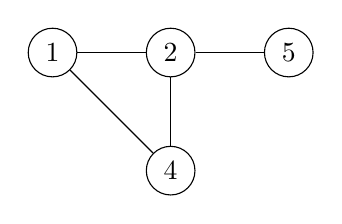
\begin{tikzpicture}[node distance=1.5cm, every node/.style={draw, circle}]
            % Define Nodes
            \node (1) {1};
            \node (2) [right of=1] {2};
            \node (4) [below of=2] {4};
            \node (5) [right of=2] {5};
            
            % Draw Edges
            \draw (1) -- (2);
            \draw (2) -- (4);
            \draw (1) -- (4);
            \draw (2) -- (5);
        \end{tikzpicture}
    \end{minipage}%
    \begin{minipage}{0.45\textwidth}
        \vspace*{0.1cm} % Adjust this value to fine-tune vertical alignment
        \[
        \mathbf{A} = \begin{bmatrix}
            0 & 1 & 1 & 0 \\
            1 & 0 & 1 & 1 \\
            1 & 1 & 0 & 0 \\
            0 & 1 & 0 & 0 \\
        \end{bmatrix}
        \]
    \end{minipage}
    \caption[Example of an undirected graph]{A simple undirected graph $G$ on $V$, with $V=\{1,2,4,5\}$ and $E(G)=\{\{1,2\},\{2,4\},\{1,4\},\{2,5\}\}$ (left), and its adjacency matrix $\mathbf{A}$ (right).}
    \label{fig:graph-example}
\end{figure}

\begin{figure}[h]
    \centering
    \begin{tikzpicture}[
        every node/.style={circle, draw, minimum size=1cm},
        on grid,
        node distance=2cm
    ]
        % Define nodes in two color classes
        \node[fill=blue!20] (u1) at (0,0) {1};
        \node[fill=blue!20] (u2) at (2,0) {2};
        \node[fill=blue!20] (u3) at (4,0) {3};

        \node[fill=red!20] (v1) at (1,-2) {a};
        \node[fill=red!20] (v2) at (3,-2) {b};

        % Edges between classes
        \draw (u1) -- (v1);
        \draw (u1) -- (v2);
        \draw (u2) -- (v1);
        \draw (u3) -- (v2);
    \end{tikzpicture}
    \caption[Example of a bipartite graph]{A bipartite graph with color classes $V_1 = \{1,2,3\}$ (blue) and $V_2=\{a,b\}$ (red).}
    \label{fig:bipartite-colored}
\end{figure}

\textbf{Random Graphs}
\label{sec:random-graphs}

%Gilbert\cite{} describes the process of generating a random graph of order $N$ by assigning a common probability to exist in the graph to each potential edge between two nodes. Note that these random selections are made independently of each other, effectively drawing from a Bernoulli distribution. \\
Gilbert \cite{gilbert1959random} describes the process of generating a random graph of order $N$ by assigning a common probability of existence to each potential edge between any two nodes. For each of these potential edges an experiment is performed independently to determine whether it shall be included in the resulting graph. Note that this process can be modeled using a Bernoulli distribution.
%The actual edges in the graph are then selected by performing random experiments, made independently of each other, and can therefore be described by a Bernoulli distribution.
%Note that these random selections are made independently of each other and effectively drawn from a Bernoulli distribution.

%Version 1 (probability space for PGE not needed, definition for one random graph suffices?): \\
A random graph is further described by Diestel \cite{Diestel2017}[p.323] as follows. Let $V = \{0,...,n-1\}$ be a fixed set of $n$ elements. Say we want to define the set $\mathcal{G}$ of all graphs on $V$ as a probability space, which allows us to ask whether a Graph $G \in \mathcal{G}$ has a certain property. To generate our random graph we then decide from some random experiment whether $e$ shall be an edge of $G$ for each potential $e \in V \times V$. The probability of success - accepting $e$ as edge in $G$ - is defined as $p \in [0,1]$ for each experiment. This leads to the probability of $G$ being a particular graph $G_0$ on $V$ with e.g. $m$ edges being equal to $p^m q^{\binom{n}{2}-m}$ with $q:=1-p$.
\bigskip

%Version 2: \\
%A random graph is further described by Diestel\cite{Diestel2017}[p.323] as follows. Let $V = \{0,...,n-1\}$ be a fixed set of $n$ elements. To generate our random graph we then decide from some random experiment whether $e$ shall be an edge of $G$ for each potential $e \in V \times V$. The probability of success - accepting $e$ as edge in $G$ - is defined as $p \in [0,1]$ for each experiment. This leads to the probability of $G$ being a particular graph $G_0$ on $V$ with e.g. $m$ edges being equal to $p^m q^{\binom{n}{2}-m}$ with $q:=1-p$. It follows our desired probability space $\mathcal{G}=(n,p)$ as the product space
%\begin{equation}
%    \Omega := \prod_{e \in [V]^2} \Omega_e
%\end{equation}
%with $\Omega_e := \{0_e,1_e\}$, $\mathbb{P}_e(\{1_e\}) := p$ and $\mathbb{P}_e(\{0_e\}) := q$.
%TODO: This is probably unnecessary for PGE.
%\begin{equation}
%    E(G) = \{e | \omega(e) = 1_e\}
%\end{equation}
%E(G) = Edges of G. G is called a random graph on V with edge probability $p$. \bigskip

\section{Information Theory}
\label{sec:information_theory}
To fully understand the learning objective of PGExplainer it is necessary to define the concepts of entropy and mutual information. We follow the definitions by Cover et al. \cite{Cover2005}[p.13] if not stated otherwise.

\subsection{Entropy}
%TODO: REVISE THIS. Probably best to define with general expactation, for continous and discrete, according to Goodfellow. Derive conditional entropy for general case. Only apply discrete case where needed? (cross entropy in PGE) \bigskip

Entropy is used to describe the uncertainty of a random variable. It quantifies the average amount of information produced by the outcomes of that variable. This is commonly illustrated as the average number of bits needed to encode its values if optimal code is used. Let $X$ be a discrete random variable with alphabet $\mathcal{X}$ and probability mass function $p(x)=Pr\{X=x\}$ for $x\in X$. TODO: EINHEITLICHE DEFINTION! SIMPLY USE THIS DEFINITION IN MONTE CARLO SAMPLING?
The entropy $H(X)$, also written as $H(p)$, is defined as
\begin{equation}
    H(X) = -\sum_{x \in \mathcal{X}} p(x) \log p(x).
\end{equation}
%TODO: WE USE NATURAL LOGARITHM IN CODE!
The log is to the base $e$ and entropy is measured in nats in our case. We will use the convention from Cover et al. \cite{Cover2005} that $0 \log 0 = 0$, as terms of zero probability do not change the entropy. %A simple example is tossing two coins: There are four possible outcomes $\mathcal{X}=\{00,10,01,11\}$, 0 for heads and 1 for tails, each with a probability $p=0,25$. The resulting entropy $H(X)=2$ represents that two bits of information can be stored this way. \bigskip
\\
%TODO: DIFFER MORE CLEARLY FROM CROSS? \\
%Analogously we define the joint entropy $H(X,Y)$ of a pair of discrete random variables $(X,Y)$ with a joint distribution $p(x,y)$ as follows:
%\begin{equation}
%    H(X,Y)=-\sum_{x \in \mathcal{X}} \sum_{y \in \mathcal{Y}} p(x,y) \log p(x,y).
%\end{equation}
The conditional entropy of $Y$ given $X$ is defined as the expected value of the entropies of the conditional distributions, averaged over the conditioning random variable. If $(X,Y) \sim p(x,y)$ for a pair of discrete random variables $(X,Y)$ with joint distribution $p(x,y)$, the conditional entropy is defined as
\begin{align}
    H(Y|X)&= -\sum_{x \in \mathcal{X}} p(x) H(Y|X=x) \\
    &= - \sum_{x \in \mathcal{X}} \sum_{y \in \mathcal{Y}}p(x,y) \log p(y|x) \\
    &= -\mathbb{E} \log p(Y|X).
\end{align}

\subsection{Relative Entropy and Cross-Entropy}
%Elements of Information Theory: equation 2.26 describes KL distance/relative entropy \bigskip
The relative entropy between two distributions is a measure of "distance" between the two. It measures the inefficiency of assuming a distribution to be $q$ when the true distribution is $p$. Note that it is not a true measure of distance as it is not symmetrical. The relative entropy takes a value of $0$ only if $p = q$.
We define the KL divergence or relative entropy between two probability mass functions $p(x), q(x)$ as
\begin{equation}
    D_{KL}(p||q) = \sum_{x \in \mathcal{X}} p(x)\log \frac{p(x)}{q(x)}.
\end{equation}
We use the convention from Cover et al. \cite{Cover2005} that $0 \log \frac{0}{0} = 0$, $0 \log \frac{0}{q} = 0$ and $p \log \frac{p}{0} = \infty$.
Suppose we know the true distribution $p$ of our random variable. We could then construct a code with an average description length of $H(p)$. If we used the code for the distribution $q$ instead, we would need $H(p) + D_{KL}(p||q)$ nats to describe the random variable on average. This is also referred to as the cross-entropy (see Goodfellow et al. \cite{Goodfellow-et-al-2016}[p.74]):
\begin{equation}
    H(p,q) =  H(p) + D_{KL}(p||q)
\end{equation}


%The following definitions loosely follow Goodfellow et al.\cite{Goodfellow-et-al-2016}[p.74].
%The relative entropy is a measure of the distance between two distributions.
%"measure how different these two distributions are" \cite{Goodfellow-et-al-2016}
%"In the case of discrete variables, it is the extra amount of information needed to send a message containing symbols drawn from probability distribution P, when we use a code that was designed to minimize the length of messages drawn from probability distribution Q."
%"The KL divergence is 0 if and only if P and Q are the same distribution in the case of discrete variables"
%non symmetrical.
%"When computing many of these quantities, it is common to encounter expressions of the form 0 log 0. By convention, in the context of information theory, we treat these expressions as limx→0 x log x = 0. \\
%We define the KL divergence or relative entropy between two probability distributions $P, Q$ as
%\begin{equation}
%    D_{KL}(P||Q) = \sum_{x \in \mathcal{X}} P(x)\log \frac{P(x)}{Q(x)}
%\end{equation}

%The cross entropy is closely related to KL distance and therefore defined as
%\begin{align}
%    H(P,Q) &= -\mathbb{E}_{x\sim P}\log Q(x) \\
%    &= H(P) + D_{KL}(P||Q)
%\end{align}

Since this is later applied in the PGExplainer (see Equation \ref{eq:monte_carlo}), we derive for the discrete case with mass probability functions $p, q$ defined on the same support $\mathcal{X}$:
\begin{align}
    H(p,q) = H(p) + D_{KL}(p||q) &= -\sum_{x \in \mathcal{X}} p(x) \log p(x) + \sum_{x \in \mathcal{X}} p(x)\log \frac{p(x)}{q(x)} \\
    &= -\sum_{x \in \mathcal{X}} p(x) \log p(x) + \sum_{x \in \mathcal{X}} p(x) \log p(x) -\sum_{x \in \mathcal{X}} p(x) \log q(x) \\
    &= -\sum_{x \in \mathcal{X}} p(x) \log q(x)
\end{align}

\subsection{Mutual Information}
%(see Cover et al.\cite{Cover2005}[p.19])
A closely related concept is mutual information. It measures the amount of information that one random variable contains about another or the reduction in uncertainty of said variable due to knowing the other. A high mutual information therefore implies that the information of one variable can be gathered from the other.

Let $X$ and $Y$ be two random variables with the joint probability mass function $p(x,y)$ and marginal probability mass functions $p(x)$ and $p(y)$. Mutual information $I(X;Y)$ is the relative entropy between the joint distribution and the product distribution $p(x)p(y)$: 
\begin{align}
    I(X;Y)&=\sum_{x \in \mathcal{X}}\sum_{y \in \mathcal{Y}} p(x,y)\log \frac{p(x,y)}{p(x)p(y)} \\
    &= H(X) - H(X|Y)
\end{align}

\section{Graph Neural Networks}
\label{sec:gnns}

Graph Neural Networks(GNNs) \cite{4700287} are a DL-based approach that operates on graphs. Due to their unique non-Euclidean property they find usage in many areas, including node classification \cite{gao2019graph}, graph classification \cite{xu2018powerful} and link prediction tasks \cite{zhang2018link}. Their high interpretability and strong performance have led to GNNs becoming a commonly employed method in graph analysis. They combine the key features of convolutional neural networks \cite{726791}, such as local connection, shared weights, and multi-layer usage, with the concept of graph embeddings \cite{cai2018comprehensive} to leverage the power of feature extraction and representation as low-dimensional vectors for graphs (see Liu et al. \cite{Liu2020}).\bigskip

TODO: CONCRETELY DEFINE NODE AND GRAPH TASKS!
Graphs are a common way of representing data in many different fields, including ML. ML applications on graphs can mostly be divided into graph-focused tasks and node-focused tasks. For graph-focused applications our model does not consider specific singular nodes, but rather implements a classifier on complete graphs. In node-focused applications however the model is dependent on specific nodes, leading to classification tasks that rely on the properties of each node.
The study of GNNs was first introduced in \cite{gori2005new} and refined in \cite{4700287}. Thus, we describe the supervised GNN model by Scarselli et al. \cite{4700287} that aims to preserve the important, structural information of graphs by encoding their topological relationships among nodes. 

A node is naturally defined by its features as well as its related notes in the graph. The goal of a GNN is to learn state embeddings $\mathbf{h}_v \in \mathbb{R}^S$ for each node $v$, that map the neighborhood of a node into a representation. These embeddings are used to obtain outputs $\mathbf{o}_v$, that e.g. may contain the distribution of a predicted node label. The GNN model proposed by Scarselli et al. \cite{4700287} uses undirected homogeneous graphs with $\mathbf{x}_v$ describing the $d$-dimensional features of each node and $x_e$ the optional features of each edge. The model updates the node states according to the input neighborhood with a local transition function $f$ that is shared by all nodes. Additionally, the local output function $g$ is used to produce the output of each node. $\mathbf{h}_v$ and $\mathbf{o}_v$ are therefore defined as
\begin{equation}
    \mathbf{h}_v = f(\mathbf{x}_v, \mathbf{x}_{E(v)}, \mathbf{h}_{\mathcal{N}(v)}, \mathbf{x}_{\mathcal{N}(v)}),
    \label{eq:gnn_state_local}
\end{equation}
\begin{equation}
    \mathbf{o}_v = g(\mathbf{h}_v, \mathbf{x}_v),
\end{equation}
with $\mathbf{x}$ denoting input features and $\mathbf{h}$ the hidden state. $\mathbf{x}_v, \mathbf{x}_{E(v)}, \mathbf{h}_{\mathcal{N}(v)}, \mathbf{x}_{\mathcal{N}(v)}$ denote the features of the node $v$ and of its incident edges, as well as the states and features of its neighboring nodes, respectively. We define $\mathbf{H}, \mathbf{O}, \mathbf{X} \text{ and  }\mathbf{X}_N$ as the matrices that are constructed by stacking all states, outputs, features, and node features, respectively. This allows us to define with the global transition function $F$ and the global output function $G$, which are stacked versions of their local equivalent for all nodes in a graph: 
\begin{equation}
    \mathbf{H} = F(\mathbf{H}, \mathbf{X}),
    \label{eq:gnn_state_global}
\end{equation}
\begin{equation}
    \mathbf{O} = G(\mathbf{H},\mathbf{X}_N).
\end{equation}
Note that $F$ is assumed to be a contraction map and the value of $\mathbf{H}$ is the fixed point of equation \eqref{eq:gnn_state_global}. To compute the state the iterative scheme
\begin{equation}
    \label{eq:GNN_iterations}
    \mathbf{H}^{t+1} = F(\mathbf{H}^t, \mathbf{X})
\end{equation}
is used with $\mathbf{H}^t$ denoting iteration t of $\mathbf{H}$. The computations of $f$ and $g$ can be understood as the feedforward neural network. \\
To learn the parameters of this GNN, with target information $t_v$ for a specific node $v$, the loss is defined as
\begin{equation}
    loss = \sum_{i=1}^p (t_i-\mathbf{o},)
\end{equation}
where $p$ are the supervised nodes. A gradient-descent strategy is utilized in the learning algorithm, which consist of the following three steps: the states $h_v^t$ are updated iteratively using equation \eqref{eq:gnn_state_local} until time step $T$. We then obtain an approximate fixed point solution of equation \eqref{eq:gnn_state_global}: $\mathbf{H}(T)\approx\mathbf{H}$. For the next step the gradients of the weights $W$ are calculated from the loss. Finally, the weights $W$ are updated according to the computed gradient. This allows us to train a model for specific supervised or semi-supervised tasks, referred to as downstream task, and get hidden states of nodes in a graph. \bigskip

Though the architecture proposed by Scarselli et al. \cite{4700287} proved to be powerful for modeling structural data, this initial approach suffers from a few limitations. Most notably, it uses the same parameters in the iteration, while nowadays it is common practice to use different parameters in different layers. Stacking $k$ GNN layers allows each node to aggregate information from nodes within its $k$-hop neighborhood, represented in Figure \ref{fig:k-hop}, seeking an increase in performance. It is important to note that this approach may also increase the noisy information spread by the exponentially increasing neighborhood nodes \cite{Liu2020}.

Another drawback is the computational inefficiency, as hidden states have to be updated $T$ times until reaching the fixed point. A relaxation of the fixed point assumption enables multi-layer GNNs to provide stable representations of the node and its neighborhood \cite{li2015gated}. Additionally, this architecture is unable to model informative edge features, which limits its capacity to learn meaningful hidden representations for edges.


TODO: MOVE AFTER TWO SPECIFIC LAYERS? DEFINE GCN AS MPNN AS EXAMPLE, EVEN IF NOT USED? MAINLY NEEDED FOR RATIONALITY OF NEUROSAT BEING GNN

The Message Passing Neural Network (MPNN) proposed by Gilmer et al. \cite{gilmer2017neural} seeks to unify GNN models, by providing a general framework for supervised learning on GNNs, since many existing models operate similarly. Typically, messages derived from node features are passed along edges of a graph to be able to learn meaningful graph and node representations that can be used for downstream tasks \cite{kipf2016semi} \cite{4700287} \cite{velivckovic2017graph} \cite{xu2018powerful}. Therefore, GNNs may be expressed as MPPNs, where the forward pass consist of a message passing phase and a readout phase. The message passing phase runs for $T$ time steps and is defined by the message function $M_t$, as well as the node update function $U_t$. At each time step $t$, the hidden state $\mathbf{h}_v^{t+1}$ of a node $v$ in the graph $G$ is updated based on the message $\mathbf{m}_v^{t+1}$, which aggregates information from the previous hidden states of its neighbors according to the message function $M_t$. Formally, this is defined as

\begin{align}
    \mathbf{m}_v^{t+1} &= \sum_{w \in \mathcal{N}(v)} M_t\left(\mathbf{h}_v^t, \mathbf{h}_w^t, \mathbf{e}_{v,w}\right) \tag{1} \\
    \mathbf{h}_v^{t+1} &= U_t\left(\mathbf{h}_v^t, \mathbf{m}_v^{t+1}\right) \tag{2},
\end{align}
where $\mathbf{e}_{v,w}$ denotes possible edge features of edge $(v,w)$.
In the readout phase a feature vector $\hat{\mathbf{y}}$ is computed for the entire graph from the final node states  using a readout function $R$:
\begin{equation}
    \hat{\mathbf{y}} = R\left(\{ \mathbf{h}_v^T \mid v \in G \}\right) \tag{3}.
\end{equation}
Note that the three functions $M_t$, $U_t$ and $R_t$ are learned and differentiable.
    
Example Kipf and Welling:
\begin{equation}
    M_t(\mathbf{h}_v^t, \mathbf{h}_w^t) = c_{v,w}\mathbf{h}_w^t,
\end{equation}
with $c_{v,w} = (d(v)d(w))^{-\frac{1}{2}}\mathbf{A}_{v,w}$.
\begin{equation}
    U_v^t(\mathbf{h}_v^t, \mathbf{m}_w^{t+1}) = \text{ReLU}(\mathbf{W}^t\mathbf{m}_v^{t+1}).
\end{equation}







Therefore, we briefly present two subsequent models that are used in the course of this work.


\tikzstyle{texts} = [text centered, font=\small, draw=none]
\begin{figure}
    \centering
    \begin{tikzpicture}[scale=1.2, every node/.style={circle, draw, minimum size=8mm, inner sep=1pt}]
        % Central node
        \node[fill=blue!30] (u) at (0,0) {$u$};
    
        % 1-hop neighbors (green)
        \foreach \i/\name in {0/v1, 90/v2, 180/v3, 270/v4} {
            \node[fill=green!30] (\name) at (\i:2) {$\name$};
            \draw (u) -- (\name);
        }
    
        % 2-hop neighbors (yellow)
        \foreach \i/\name in {20/w1, 110/w3, 160/w4, 200/w5, 250/w6, 290/w7, 340/w8} {
            \node[fill=yellow!30] (\name) at (\i:3.5) {$\name$};
        }
    
        % Connections from 1-hop to 2-hop
        \foreach \parent/\child in {v1/w1, v2/w3, v2/w4, v3/w5, v3/w6, v4/w7, v4/w8} {
            \draw (\parent) -- (\child);
        }

        % Highlight 2-hop neighborhood
        \begin{scope}[on background layer]
            \fill[yellow!10] (0,0) circle (4);
            \fill[green!10] (0,0) circle (2.4);
        \end{scope}

        % Labels directly on the rings
        \node[texts, font=\small] at (45:2.4) {1-hop neighborhood};
        \node[texts, font=\small] at (45:4) {2-hop neighborhood};
        
    \end{tikzpicture}
    \caption[$k$-hop neighborhood visualization]{Visualization of the $k$-hop neighborhood of $u$.}
    \label{fig:k-hop}
\end{figure}

\textbf{Graph Convolutional Network} \\
Graph convolutional networks (GCNs) aim to generalize the convolution operation of convolutional neural networks (CNNs) to the graph domain. An example is the model proposed by Kipf et al. \cite{kipf2016semi} that introduces a simple, layer-wise propagation rule for multi-layer GCNs as
\begin{equation}
    \label{eq:GCN}
    H^{l+1} = \sigma(\tilde{D}^{-\frac{1}{2}}\tilde{A}\tilde{D}^{-\frac{1}{2}}H^{(l)}W^{(l)}),
\end{equation}
where $\tilde{A} = A + I_N$ is the adjacency matrix of the undirected input graph $G$ with added self-connections. $I_N$ is the identity matrix, $\tilde{D}$ is the degree matrix and $W^{(l)}$ is a layer-specific trainable weight matrix. $\sigma(\cdot)$ denotes an activation function, such as ReLU. $H^{(l)} \in \mathbb{R}^{n\times d}$ denotes the matrix of node activations in the $l$-th layer, where $H^{(0)} = X$. Note that this definition differs slightly from the iterative formulation in Equation \ref{eq:GNN_iterations}, in the sense that each layer applies a different function $F_l$, rather than a shared function $F$. $\tilde{D}^{-\frac{1}{2}}\tilde{A}\tilde{D}^{-\frac{1}{2}}$ describes a normalization of the adjacency matrix, referred to as renormalization trick. This architecture aims to alleviate the problem of overfitting on local neighborhood structures for graphs with very wide node degree distributions (TODO: Source).

%TODO: generalization to signal X?
%\begin{equation}
%    Z = \hat{D}^{-\frac{1}{2}}\hat{A}\hat{D}^{-\frac{1}{2}}X\Theta
%\end{equation}

\textbf{Higher-order GNN} \\
TODO: A basic GNN model can be implemented as follows (Hamilton, Ying, and Leskovec 2017b)
Morris et al. \cite{morris2019weisfeiler} propose an implementation for a GNN model consisting of stacked neural network layers, that each aggregate the local neighborhood information of a node and pass it to the next one. This network is defined specifically for graphs that can be partitioned into $r$ color classes and therefore applicable to bipartite graphs. The new features of node $i$ are then computed with:
\begin{equation}
    \label{eq:higher-order-gnn}
    x_i^{(l)} = \sigma(W_1^{(l)}x_i^{(l-1)}+W_2^{(l)}\cdot\sum_{j\in\mathcal{N}(i)}e_{j,i}\cdot x_j^{(l-1)}),
\end{equation}
where $W_1^{(l)}$ and $W_2^{(l)}$ are two layer-specific trainable weight matrices.

%No activation: x_i' = W_1x_i+W_2 \sum_{j\in\mathcal{N}(i)}e_{j,i}\cdot x_j \\
TODO: MORE MOTIVATION FOR THIS!


\section{Boolean Satisfiability Problem}
\label{sec:SAT}
We define the Boolean Satisfiability Problem (SAT) according to Guo et al. \cite{guo2023machine}[p.641]: \\
A Boolean formula is constructed from Boolean variables, that only evaluate to True (1) or False (0), and the three logic operators conjunction ($\wedge$), disjunction ($\vee$) and negation ($\neg$). SAT aims to evaluate whether there exists a variable assignment for a formula constructed of said parts so that it evaluates to True. If so, the formula is said to be satisfiable or unsatisfiable otherwise. Every propositional formula can be converted into an equivalent formula in conjunctive normal form (CNF), which consists of a conjunction of one or more clauses. These clauses must contain only disjunctions of at least one literal (a variable or its negation). In this work we consider only formulas in CNF, as NeuroSAT \cite{selsam2018learning} assumes SAT problems to be in CNF. An example of a satisfiable formula in CNF over the set of variables $V=\{x_1,x_2\}$ is 
$$\psi(V) = (x_1) \land (\neg x_1 \lor x_2) \land (\neg x_2 \lor x_2)$$
with satisfying assignment $A:\{x_1 \mapsto 1, x_2 \mapsto 1\}$. Furthermore, SAT is $NP$-complete, meaning that if there exists a deterministic algorithm able to solve SAT in polynomial time, then such an algorithm exists for every $NP$ problem (see cook \cite{cook2023complexity}). Current state-of-the-art SAT solvers apply searching based methods such as Conflict Driven Clause Learning \cite{marques1999grasp} or Stochastic Local Seach \cite{selman1993local} with exponential worst-case complexity.

\subsection{Representation as Bipartite Graph}
SAT has extensively been studied in the form of graphs. Guo et al. \cite{guo2023machine} describe four different types of graph representations for CNF formulae with varying complexity and information compression. Since we want to minimize the loss of information for SAT we adapt the information-richest form of a literal-clause graph (LCG). 
A LCG is a bipartite graph that separates literals and clauses, with edges connecting literals to the clauses they appear in (see Figure \ref{fig:lcg-sat}).
The resulting graph $G_b$ can formally be described by a biadjacency matrix $\mathbf{B}$ of shape $L \times C$, with $(L,C)$ being a bipartition of the $G_b$ into literals and clauses. \\
Following Sun et al. \cite{articleBiadjacency}, let $\mathbf{A} \in \mathbb{R}^{(L+C) \times (L+C)}$ be the adjacency matrix of our bipartite graph. Since for the bipartite case edges exist only between the two color classes $L$ and $C$, the adjacency matrix can be represented as
\begin{equation}
    \mathbf{A}(i,j) = \begin{bmatrix}
        \mathbf{0}_{L \times L} & \mathbf{B} \\
        \mathbf{B}^T & \mathbf{0}_{C \times C}
    \end{bmatrix},
\end{equation}
where $\mathbf{0}$ denotes a zero matrix in the shape of their subscript. \bigskip

\begin{figure}[h]
    \centering
    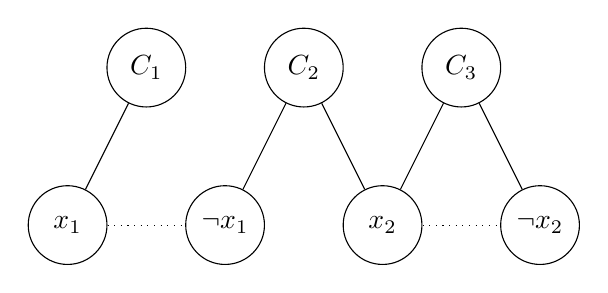
\begin{tikzpicture}[
        every node/.style={draw, circle, minimum size=1cm},
        node distance=1.5cm,
        scale=0.8,
    ]
        % Define Literal Nodes
        \node (x1) at (0, 0) {\(x_1\)};
        \node (notx1) at (2.5, 0) {\(\neg x_1\)};
        \node (x2) at (5, 0) {\(x_2\)};
        \node (notx2) at (7.5, 0) {\(\neg x_2\)};
        
        % Define Clause Nodes (one level above literals)
        \node[circle, draw] (C1) at (1.25, 2.5) {\(C_1\)};
        \node[circle, draw] (C2) at (3.75, 2.5) {\(C_2\)};
        \node[circle, draw] (C3) at (6.25, 2.5) {\(C_3\)};
        
        % Draw Edges (Literal → Clause)
        \draw (x1) -- (C1);
        \draw (notx1) -- (C2);
        \draw (x2) -- (C2);
        \draw (notx2) -- (C3);
        \draw (x2) -- (C3);
        
        % Draw Dotted Edges between each literal and its co mplement
        \draw[dotted] (x1) -- (notx1);
        \draw[dotted] (x2) -- (notx2);
    \end{tikzpicture}
    \caption[Bipartite graph in LCG]{LCG representation of $\psi(V)$ with dashed lines representing the connection between complementary literals relevant for the message passing in GNNs.}
    \label{fig:lcg-sat}
\end{figure}

%\subsection{Incidence/Levi graph?}
%Defined in ALYAHYA et al. Concrete graphical representation of SAT? Type of bipartite graph.
%Defines edges via edge weight function! PART OF GRAPH THEORY \\
%Definition in Cimatti et al. : For clause $c$ we use $lit(c)$ and $var(c)$ to reference the %set of literals and variables in $c$ respectively. "$For a CNF formula F we write
%cla(F) for its set of clauses, lit(F)= c \in cla(F) lit(c) for its set of literals, and
%var(F)= c \in cla(F) var(c) for its set of variables.$"  Incidence graph of $\psi$ is the %bipartite graph $inc(\psi) = (V,E)$ with $V=lit(\psi) \cup cla(\psi)$. Additionally for %literal $x \in lit(\psi)$ and clause $c \in cla(\psi)$ we define $xc \in E$ if $x \in var(c)$.

\subsection{Unsatisfiable Cores}
The core of an unsatisfiable formula in CNF is a subset of the formula that is also unsatisfiable. Every unsatisfiable formula therefore is a core on its own, but can be broken down into smaller cores. The smaller a core the more significance it holds. A minimal unsatisfiable core is also referred to as a minimal unsatisfiable subset (MUS). SAT solvers like minisat \cite{een2003extensible} are able to compute unsatisfiable cores but do not generally provide a MUS due to high computational cost. However, several deletion-based algorithms exist for computing MUSs (see Torlak et al. \cite{10.1007/978-3-540-68237-0_23}).
    \chapter{Related Work}

%Propose only using PGExplainer for Node classification task.\bigskip
Yuan et al. \cite{yuan2022explainability} performed an extensive taxonomic survey on explainability in graph neural networks. We use this survey to discuss different approaches and motivate the selection of the PGExplainer in \ref{sec:gnn_explainability}. The authors note that the PGExplainer "is not performing as promising as its original reported results" \cite{yuan2022explainability}. Nevertheless, we evaluate the explainer model with regard to its applicability in the inductive setting. In \ref{sec:Explainer_Models} we briefly introduce important work related to the PGExplainer, as well as the model itself, since it is the core of our work. Lastly, we refer to NeuroSAT, which we use as a downstream model for the PGExplainer to generate explanations for its predictions on the SAT problem in \ref{sec:Downstream_Models}.

\section{Explainability in GNNs}
\label{sec:gnn_explainability}

Methods in DL have seen growth in performance in many tasks of artificial intelligence, including GNNs, since graphs are able to capture real-world data such as social networks or chemical molecules \cite{ying2018graph}, \cite{ma2021deep}. However, the interpretability of these models is often limited due to their black-box design \cite{noor2024survey}. Explainability methods aim to bypass this limitation by designing post-hoc techniques that provide insights into the decision-making process in the form of explanations. Such human-intelligible explanations are crucial for deploying models in real-world applications, especially when applied in interdisciplinary fields \cite{ribeiro2016should}.

There exist several different approaches for explaining predictions of deep graph models, that can be categorized into instance-level methods and model-level methods (see Yuan et al.  \cite{yuan2022explainability}). Instance-level methods aim to explain each input-graph by identifying important input features for its prediction, leading to input-dependent explanations. These can further be grouped by their importance score calculation into four branches. Gradients/feature-based methods use gradients as approximations of importance scores. Sensitivity Analysis \cite{baldassarre2019explainability} is an example that directly uses squared values of gradients as importance scores of input features. This enables the scores to be calculated directly with back-propagation.

Perturbation-based approaches like GNNExplainer \cite{ying2019gnnexplainer} and PGExplainer \cite{luo2020parameterized} study the variation of the output with regard to different input perturbations. The intuition behind this is that when input information crucial to the prediction is kept, the new prediction should roughly align with the prediction from the original input. PGExplainer aims to improve the GNNExplainer by providing a way of generating explanations with a global understanding of the GNN, significantly improving the computational cost. Another approach is SubgraphX \cite{yuan2021explainability}, which utilizes Monte Carlo Tree search to generate subgraph-level explanations. This does however entail a higher computational cost. 

Surrogate methods for deep graph models are inspired by surrogate methods for image data, that rely on neighboring areas of an input. Since graph data is concrete and contains topological information it is difficult to define the neighboring regions of an input graph. The idea is to obtain a local dataset containing neighboring data objects and predictions and fitting a simple, interpretable surrogate model to learn the local dataset. The explanations of the surrogate model are then regarded as the explanations of the original model. GraphLime \cite{huang2022graphlime} is an example that considers the $N$-hop neighboring nodes of a target node as the local dataset, where $N$ may be the number of GNN-layers. The weighted features of a non-linear surrogate model are then regarded as explanations. However, this method only explains node features, rather than the graph structure.

Decomposition methods, also motivated by success in the image domain, aim to measure input feature importance by decomposing the prediction into several terms, regarded as feature dependant importance score. Approaches for deep graph neural networks, like Layer-wise Relevance Propagation \cite{baldassarre2019explainability}, decompose the output prediction score to node importance scores. The decomposition rule is based on hidden features and weights, only enabling the study of node importance rather than graph structures.

Model-level methods, on the other hand, aim to explain GNNS without considering specific inputs, leading to input-independent, high-level explanations.


To fully trust the explanations provided by an explainer model, they must satisfy certain criteria, since there often is a mismatch between the optimizable metrics like accuracy and the actual metric of interest, which may not be measurable (see Ribeiro et al. \cite{ribeiro2016should}). First and foremost, an explanation should be \textbf{interpretable} and therefore provide qualitative, human-understandable interpretations, that also consider the possibility of limited user knowledge. Additionally, \textbf{local fidelity} asserts that explanations should be faithful in a local context and consider the models' behavior in the vicinity of predicted instances. Explainers that treat the model to be explained as a black-box are \textbf{model-agnostic} and should therefore be able to explain any model. Lastly, a \textbf{global perspective} is needed to explain a model fully, allowing us to take sample explanations of individual predictions that serve as representation of the model.

TODO: Claims to satisfy?
Since the perturbation-based PGExplainer \cite{luo2020parameterized} claims to satisfy all the criteria, while also maintaining reasonable computational cost, we select this model for the course of this study. It is furthermore able to generate explanations in an inductive setting, which we aim to do in \ref{}.

The general pipeline for different perturbation based approaches can be described as follows: First, the important features from the input graph are converted into a mask by our generation algorithm, depending on the explanation task at hand. These masks are applied to the input graph to highlight said features. Lastly, the masked graph is fed into the trained GNN to evaluate the mask and update the mask generation algorithm according to the similarity of the predictions. 

These different approaches mostly differ in the specific mask generation algorithm, the type of mask used and the objective function. It is important to distinguish between soft masks, discrete masks and approximated discrete masks. Soft masks take continuous values between $[0,1]$ which enables the graph algorithm to be updated via backpropagation. A downside of soft masks is that they suffer from the "introduced evidence" problem (see Dabkowski et al. \cite{dabkowski2017real}). Any mask value that is non-zero or non-one may add new semantic meaning or noise to the input graph, since graph edges are by nature discrete. Discrete masks however always rely on non-differentiable operations, e.g. sampling. Thus, the approximated discrete masks utilize reparameterization tricks to avoid the "introduced evidence" problem while also enabling back-propagation. %TODO: Expand on reparameterization trick?

Explanations can on the one hand be evaluated by visualizing the graph and considering the "human-comprehensibility". Since this requires a ground truth, is prone to the subjective understanding and is usually performed for a few random samples, it is important to apply stable evaluation metrics. One relevant accuracy metric for synthetic datasets with ground truths is the Area Under the Receiver Operating Characteristic Curve (ROC-AUC) (see Richardson et al. \cite{RICHARDSON2024100994}). The Receiver Operating Characteristic (ROC) curve plots the False Positive Rate (FPR) on the x-axis against the True Positive Rate (TPR), across different classification thresholds. The area under the curve (AUC) is calculated for said curve, resulting in the ROC-AUC. It is important to note, that a value of $0.5$ equals random guessing, while a score of $1.0$ indicates perfect classification. TODO: Other metrics include fidelity, results of taxonomy propose only using PGExplainer for Node Classification as it achieves low fidelity on Graph tasks

TODO: figure of perturbation pipeline?


\section{TODO: SECTION NAME Explainer Models}
\label{sec:Explainer_Models}

\textbf{GNNExplainer} \\
Ying et al. proposed the GNNExplainer \cite{ying2019gnnexplainer}: the first general, model-agnostic explainer for graph neural networks on any graph-based machine learning task. It is able to identify a concise subgraph structure and a subset of node features, that play a crucial role in the prediction of the underlying graph neural network. This is generally understood as an explanation. The work by Ying et al. serves as the main baseline for the PGExplainer, that seeks to improve its predecessor. Many concepts, experiments and specifications of PGExplainer were adapted from the GNNExplainer, which we seek to process in our work. \bigskip

\textbf{Parameterized Explainer for Graph Neural Networks} \\
The Parameterized Explainer for Graph Neural Networks (PGExplainer) by Lou et al. \cite{luo2020parameterized} is the main subject of our work. The method adopts a deep neural network to parameterize the generation process of explanations, thus allowing multiple instances to be explained collectively. Furthermore, it has better generalization ability and can explicitly be utilized in an inductive setting.

We reimplement the original work using PyTorch \cite{paszke2019pytorch} and PyTorch Geometric \cite{Fey/Lenssen/2019} instead of TensorFlow \cite{tensorflow2015-whitepaper}, while also emphasizing its application in an inductive setting, where test instances are unseen during training, as opposed to the original collective setting. A secondary study on the inductive performance was also performed by the authors, which we want to extend by applying it on a graph neural network with a slightly different architecture, testing whether the explainer proves to be model-agnostic. This extension is motivated by the need for explainability methods that generalize across architectures (TODO: SOURCE FOR THIS). The goal of this thesis is to apply the explainer model to a deep learning approach for solving a bipartite graph problem - specifically, the boolean satisfiability problem - and generate proofs for the deep model's predictions. \bigskip

\textbf{[Re] Parameterized Explainer for Graph Neural Network} \\
%We try own reimplementation that follows the original paper, as well as code and reimplementation for uncertainties + use a slightly different architecture in underlying GNN + Hyperparameter search of combination of parameters used in original and repication. Treated as additional baseline

Holdijk et al. \cite{holdijk2021re} performed a replication study on the PGExplainer that focuses on reimplementing the method in PyTorch, testing whether the claims with respect to the GNNExplainer hold and discussing whether the used evaluation method makes sense. They highlight a large discrepancy between the paper and codebase, making a replication that includes the evaluation method from the paper alone impossible. With help of the codebase, the authors are able to replicate the experiments and verify the main claims of the original paper. However, they express some concerns regarding the evaluation setup and note a large difference between the originally noted AUC scores and their results for most of the datasets. Additionally, they question the general approach for evaluating graph data with ground truths, as done in GNNExplainer and PGExplainer, which we will discuss in \ref{}. We use this work as an additional baseline for our approach, but note that the replication was also done in the collective setting. Therefore, the difference to our work lies mainly in the architecture used for the downstream model and the setting of the experiments. \bigskip


\section{Downstream Model}
\label{sec:Downstream_Models}

\textbf{NeuroSAT} \\
NeuroSAT by Selsam et al. \cite{selsam2018learning} is a machine learning approach for solving the boolean satisfiability problem using a message passing neural network. It is able to detect satisfying assignments, but lacks proofs of unsatisfiability. The authors performed a small study on the detection of unsat cores, revealing that NeuroUNSAT is able to detect UNSAT cores if the UNSAT problems contain a specific UNSAT core. However, this is expected to be due to the model memorizing the unsat cores, rather than generalizing to any unsat core. We want to test this by applying the PGExplainer in an inductive setting to the NeuroSAT model, and evaluate whether the generated explanations do align with unsat cores.
    \chapter{PGExplainer - Methodology}
\label{ch:PGExplainer}
%V1: In the following chapter, we introduce the PGExplainer\cite{luo2020parameterized} and its concepts. The idea is to generate explanations in the form of probabilistic graph generative models for any learned GNN model, henceforth referred to as the downstream task (DT), by utilizing a deep neural network to parameterize the generation process. This approach seeks to explain multiple instances collectively, as they share the same neural network parameters, and therefore improve the generalizability to previous works, particularly the GNNExplainer\cite{ying2019gnnexplainer}.

%V2: In the following chapter, we introduce the PGExplainer\cite{luo2020parameterized} and its concepts. The idea is to generate explanations in the form of probabilistic graph generative models that have proven to learn the concise underlying structures of GNNs most relevant to their predictions. This approach may be applied to any learned GNN model, henceforth referred to as the downstream task (DT), by utilizing a deep neural network to parameterize the generation process. PGExplainer seeks to explain multiple instances collectively, as they share the same neural network parameters, and therefore improve the generalizability to previous works, particularly the GNNExplainer\cite{ying2019gnnexplainer}. This means that all edges in the dataset are predicted by the same model, which leads to a global understanding of the DT.

In this chapter we present the Methodology (TODO: ?) of our work, including the detailed theory of the explainer model used in our approach. Thus, we start by presenting the concept of the PGExplainer \cite{luo2020parameterized} in Section \ref{sec:TheoryPGE}.

In Section \ref{sec:NeuroSAT_extension} we present our idea of applying the PGExplainer on the NeuroSAT framework to generate explanations for a machine learning SAT-solving approach and comparing these to the "human-understandable" concept of unsatisfiable cores. 

We then describe our implementation in detail (see Section \ref{sec:implementation_details}), including the changes made and difficulties during the process, as well as the adaptations for the application on NeuroSAT.

\section{Theoretical Foundations of PGExplainer}
\label{sec:TheoryPGE}

In the following subchapter, we introduce the PGExplainer \cite{luo2020parameterized} and its concepts. The idea is to generate explanations in the form of edge distributions or soft masks using a probabilistic generative model for graph data, known for being able to learn the concise underlying structures from the observed graph data. The explainer uncovers said underlying structures, believed to have the biggest impact on the prediction of a GNNs, as explanations. This approach may be applied to any trained GNN model, henceforth referred to as the target model (TM). 

By utilizing a deep neural network to parameterize the generation process, the explainer learns to collectively explain multiple instances of a model. Since the parameters of the neural network are shared across the population of explained instance, PGExplainer provides "model-level explanations for each instance with a global view of the GNN model" \cite{luo2020parameterized}. Furthermore, this approach cannot only be used in a collective setting, but also in an inductive setting, where explanations for unexplained nodes can be generated without retraining the explanation model. This improves the generalizability compared to previous works, particularly the GNNExplainer by Ying et al. \cite{ying2019gnnexplainer} and focuses on explaining graph structure rather than graph features. \bigskip

We follow the structure of the original paper \cite{luo2020parameterized} and start by describing the learning objective in Section \ref{sec:learning_objective}, the utilized reparameterization trick in Section \ref{sec:Reparameterization_Trick}, the idea of global explanations in Section \ref{sec:Global_Explanations} and finally the applied regularization terms in Section \ref{sec:Regularization_Terms}.

\subsection{Learning Objective}
\label{sec:learning_objective}
To explain the predictions made by a GNN model for an original input graph $G_o$ with $m$ edges we first define the graph as a combination of two subgraphs: $G_o = G_s + \Delta G$, where $G_s$ represents the subgraph holding the most relevant information for the prediction of a GNN, referred to as explanatory graph. $\Delta G$ contains the remaining edges that are deemed irrelevant for the prediction of the GNN. Inspired by GNNExplainer \cite{ying2019gnnexplainer}, the PGExplainer then finds $G_s$ by maximizing the mutual information between the predictions of the target model and the underlying $G_s$:
\begin{equation}
    \max_{G_s} MI(Y_o;G_s) = H(Y_o) - H(Y_o|G=G_s),
\end{equation} 
where $Y_o$ (TODO: $\in (0,1)^c$ ??) is the prediction of the target model with $G_o$ as input and number of possible classes $c$. This quantifies the probability of prediction $Y_o$ when the input graph is restricted to the explanatory graph $G_s$, as in the case of $I(Y_o;G_s) = 1$, knowing the explanatory graph $G_s$ gives us complete information about $Y_o$, and vice versa.

Intuitively, if removing an edge $(i,j)$ changes the prediction of a GNN drastically, this edge is considered important and should therefore be included in $G_s$. This idea originates from traditional forward propagation based methods for white-box explanations (see Dabkowski and Gal \cite{dabkowski2017real}).
It is important to note that $H(Y_o)$ is only related to the target model with fixed parameters during the evaluation/explanation stage. This leads to the objective being equivalent to minimizing the conditional entropy $H(Y_o|G=G_s)$. \bigskip

To optimize this function a relaxation is applied for the edges, since normally there would be $2^m$ candidates for $G_s$. The explanatory graph is henceforth assumed to be a Gilbert random graph, where the selections of edges from $G_o$ are conditionally independent to each other. However, the authors describe a random graph with each edge having its own probability, rather than a shared probability as described in Section \ref{sec:random-graphs}, as follows: Let $e_{i,j}\in V \times V$ be the binary variable indicating whether the edge is selected, with $e_{i,j} = 1$ if edge $(i,j)$ is selected to be in the graph, and 0 otherwise. For the random graph variable $G$ the probability of a graph $G$ can be factorized as 
\begin{equation}
    P(G) = \prod_{(i,j)\in E}P(e_{i,j}).
\end{equation}
TODO: Inhomogeneous Erdős Rényi model? Mention that this is a generative model? (A Gilbert random graph is an example of a generative probabilistic model on graph data?)

 $P(e_{i,j})$ is instantiated with the Bernoulli distribution $e_{i,j} \sim Bern(\theta_{ij})$, where $P(e_{i,j} = 1) = \theta_{ij}$ is the probability that edge $(i,j)$ exists in $G$.
After this relaxation the learning objective becomes:
\begin{equation}
    \label{eq:init_learning_obj}
    \min_{G_s}H(Y_o|G = G_s) = \min_{G_s} \mathbb{E}_{G_s}[H(Y_o|G = G_s)] \approx \min_{\Theta} \mathbb{E}_{G_s \sim q(\Theta)}[H(Y_o|G = G_s)],
\end{equation}
where $q(\Theta)$ is the distribution of the explanatory graph that is parameterized by $\Theta$'s.

\subsection{Reparameterization Trick}
\label{sec:Reparameterization_Trick}
As described in Section \ref{sec:gnn_explainability}, a reparameterization trick can be utilized to relax discrete edge weights to continuous variables in the range $(0,1)$. PGExplainer uses the reparameterizable Gumbel-Softmax estimator \cite{jang2016categorical} to allow for efficiently optimizing the objective function with gradient-based methods. This method introduces the Gumbel-Softmax distribution, a continuous distribution used to approximate samples from a categorical distribution. 

A temperature $\tau$ is used to control the approximation, usually starting from a high value and annealing to a small, non-zero value. Samples with $\tau > 0$ are not identical to samples from the corresponding continuous distribution, but are differentiable and therefore allow back-propagation \cite{abid2019concrete}. The sampling process $G_s \sim q(\Theta)$ of PGExplainer is therefore approximated with a determinant function that takes as input the parameters $\Omega$, a temperature $\tau$ and an independent random variable $\epsilon$: $G_s \approx \hat{G}=f_\Omega(G_o,\tau,\epsilon)$. 

The binary concrete distribution \cite{maddison2016concrete}, also referred to as Gumbel-Softmax distribution, is utilized as an instantiation for the sampling, yielding the weight $\hat{e}_{i,j} \in (0,1)$ for edge $(i,j)$ in $\hat{G}_s$, computed by:
\begin{equation}
    \label{eq:reparam_trick}
    \epsilon \sim \text{Uniform}(0,1), \qquad \hat{e}_{i,j}=\sigma((\log \epsilon - \log(1-\epsilon)+\omega_{ij}/\tau),
\end{equation}
where $\sigma(\cdot)$ is the Sigmoid function and $\omega_{ij} \in \mathbb{R}$ is an explainer logit for the corresponding edge used as a parameter. When $\tau \rightarrow 0$, e.g. during the explanation stage, the weight $\hat{e}_{i,j}$ is binarized with the sigmoid function $\lim_{\tau\rightarrow 0}P(\hat{e}_{i,j} = 1) = \frac{e(\omega{ij})}{1+e(\omega{ij})}$. Since $P(e_{i,j} = 1) = \theta_{ij}$, choosing $\omega_{ij} = \log\frac{\theta_{ij}}{1-\theta_{ij}}$ leads to $\lim_{\tau\rightarrow 0}\hat{G}_s = G_s$ and justifies the approximation of the Bernoulli distribution with the binary concrete distribution. During training, when $\tau > 0$, the objective function in \eqref{eq:init_learning_obj} is smoothed with a well-defined gradient $\frac{\partial\hat{e}_{i,j}}{\partial\omega_{ij}}$ and becomes:
\begin{equation}
    \min_\Omega \mathbb{E}_{\epsilon \sim \text{Uniform}(0,1)}H(Y_o| G = \hat{G}_s)
\end{equation}

The authors follow the approach of GNNExplainer \cite{ying2019gnnexplainer} and modify the objective by replacing the conditional entropy with cross entropy between the label class and the prediction of the target model. This is justified by the greater importance of understanding the model's prediction of a certain class, rather than providing an explanation based solely on its confidence.

With the modification to cross-entropy $H(Y_o, \hat{Y}_s)$, where $\hat{Y}_s$ is the prediction of the target model when $\hat{G}_s$ is given as input, as well as the adaption of Monte Carlo sampling, the learning objective becomes:
\begin{equation}
    \label{eq:monte_carlo}
    \begin{aligned}
        \min_\Omega\mathbb{E}_{\epsilon\sim\text{Uniform}(0,1)}H(Y_o, \hat{Y}_s) &\approx \min_\Omega -\frac{1}{K}\sum_{k=1}^K\sum_{c=1}^C P(Y_o = c) \log P(\hat{Y}_s = c) \\
        &= \min_\Omega -\frac{1}{K}\sum_{k=1}^K\sum_{c=1}^C P_\Phi (Y_o = c|G = G_o) \log P_\Phi(\hat{Y}_s = c|G=\hat{G}_s^{(k)}).
    \end{aligned}
    \end{equation}
$\Phi$ denotes the parameters in the target model, $K$ is the number of total sampled graphs, $C$ is the number of class labels, and $\hat{G}_s^{(k)}$ denotes the $k$-th graph sampled with Equation \ref{eq:reparam_trick}, parameterized by $\Omega$. %Note that this objective is defined per explainable instance.



%The approach in PGExplainer is a common approach in ML for simplifying objectives? FIND LITERATURE THAT EXPLAINS APPROXIMATION OF COND. ENTROPY WITH CROSS ENTROPY. Explanation as simple as one formula for one graph variable example, cross entropy applied to whole distribution? \bigskip


\subsection{Global Explanations}
\label{sec:Global_Explanations}
The novelty of PGExplainer lies in the ability to generate explanations for graph data with a global perspective, that allow for understanding the general picture of a model across a population. This saves resources when analyzing large graph datasets, as new instances can be explained without retraining the model, and can also be helpful for establishing the users' trust in these explanations. To achieve this the authors propose the use of a parameterized network that learns to generate explanations from the target model, which also apply to not yet explained instances. 

Since GNNs apply two functions $F$ and $G$ to calculate the global state embeddings and downstream task outputs respectively, Luo et al. \cite{luo2020parameterized} denote these two functions as $\text{GNNE}_{\Phi_0}(\cdot)$ and $\text{GNNC}_{\Phi_1}(\cdot)$ for any GNN in the context of PGExplainer. For models without explicit classification layers the last layer is used to compute the output instead. It follows
\begin{equation}
    \mathbf{Z} = \text{GNNE}_{\Phi_0}(G_o, \mathbf{X}), \qquad Y = \text{GNNC}_{\Phi_1}(\mathbf{Z}),
\end{equation}
where $\mathbf{Z}$ denotes the matrix of final node representations $z$, referred to as node embeddings, and the initial state is $G_o$. TODO: (Because of focus on graph structure rather than features?) For generalizability across different GNN layers the output is only dependent on the node representation, that encapsulates both features and structure of the input graph. This representation also serves as the input for the explainer network $g$, defined as:
TODO: Rename g?
\begin{equation}
    \label{eq:explainer_network}
    \Omega = g_\Psi(G_o,\mathbf{Z}).
\end{equation}
$\Psi$ denotes the parameters in the explanation network and the output $\Omega$ is treated as parameter in Equation \ref{eq:monte_carlo}. Since $\Psi$ is shared by all edges among the population, PGExplainer collectively provides explanations for multiple instances. Thus, the learning objective in a collective setting with $\mathcal{I}$ being the set of instances becomes:
\begin{equation}
    \label{eq:mlp_loss}
    \min_\Psi -\frac{1}{K}\sum_{i\in \mathcal{I}}\sum_{k=1}^K\sum_{c=1}^C P_\Phi (Y_o = c|G = G_o^{(i)}) \log P_\Phi(\hat{Y}_s = c|G=\hat{G}_s^{(i,k)}).
\end{equation}
Consequently, $G^{(i)}$ and $G_s^{(i,k)}$ denote the input graph and the $k$-th graph sampled with Equation \ref{eq:reparam_trick} in \ref{eq:explainer_network} respectively for instance $i$. The full pipeline of the PGExplainer can be observed in figure \ref{fig:PGExplainer_pipeline}. 

The authors propose two slightly different instantiations of $\Omega$ for node classification and graph classification tasks.\bigskip

\textbf{Explanation Network for Graph Classification}\par
For graph level tasks, the authors consider each graph to be an instance, independent  of specific nodes. The output $\Omega$ of the network (see Equation \ref{eq:explainer_network}) is thus specified as:
\begin{equation}
    \label{eq:mlp_graph_input}
    \omega_{ij} = \text{MLP}_\Psi ([\mathbf{z}_i\oplus\mathbf{z}_j]),
\end{equation}
where $\text{MLP}_\Psi$ is an MLP (see Section \ref{sec:Replication_of_PGExplainer} for implementation details) parameterized with $\Psi$ and $\oplus$ denotes the concatenation operation. Effectively, for each edge in $G_o$ a concatenation of both its nodes is fed through the MLP. For the MLP used in both the original and this work the output $\omega_{ij}$ is an edge logit, which serves as a parameter in the sampling process. \bigskip

\textbf{Explanation Network for Node Classification}\par
%Since explanations for different nodes may not share a common explanation pattern, especially for nodes with different labels, ... DOES THIS NOT ALSO APPLY FOR GRAPHS?!
For node level tasks on the other hand, each prediction node is considered as an instance. Let an edge $(i,j)$ be considered relevant for the prediction of a node $u$, but irrelevant for the prediction of a node $v$. To explain the prediction of node $v$ the authors specify the output $\Omega$ of the network in Equation \ref{eq:explainer_network} as:
\begin{equation}
    \omega_{ij} = \text{MLP}_\Psi ([\mathbf{z}_i\oplus\mathbf{z}_j\oplus\mathbf{z}_v]).
\end{equation}
Thus, a concatenation of the node embeddings of nodes $i, j$ and $v$ respectively is fed through the network.

Note that in their codebase the authors use a concatenation of all hidden representations instead of solely the final representation as node embeddings for node level tasks.
For a target GNN consisting of $L$ graph layers with
\begin{align*}
    \mathbf{H}_1 &= F_1(G_o, \mathbf{X}), \\
    \mathbf{H}_2 &= F_2(\mathbf{H}_1, \mathbf{X}), \\
    &\vdots \\
    \mathbf{H}_L &= F_L(\mathbf{H}_{L-1}, \mathbf{X}), \\
\end{align*}
this leads to $\mathbf{Z} \in \mathbb{R}^{|V(G_o)|\times (Ld)}$ being the matrix of node embeddings $\mathbf{z}$ that are computed as:
\begin{equation}
    \mathbf{z}_i = \mathbf{h}_{1,i} \oplus \mathbf{h}_{2,i} \oplus ... \oplus \mathbf{h}_{L,i},
\end{equation}
with $\mathbf{h}_{L,i}$ denoting the hidden representations of node $i$ in layer $L$.\bigskip

Furthermore, it is important to note, that for target GNNs utilizing a message passing mechanism, the prediction at node $v$ is fully determined by its local computation graph. The local computation graph of $v$ is defined as its $L-$hop neighborhood $\mathcal{N}_L(v)$ \cite{ying2019gnnexplainer} (see Figure \ref{fig:k-hop}).\bigskip

\textbf{Collective and Inductive Setting}\par
Due to the nature of its predecessor GNNExplainer, the authors main focus was the application in a collective setting, where the goal is to explain a full population of instances by training on all these and thus being able to provide explanations for every single one. However, since the PGExplainer utilizes a deep neural network to parameterize the generation process of explanations for a population, it can be utilized in an inductive setting, unlike its predecessor. 

This means, that explanations can be generated for instances from the same population, that have not been seen during training. Thus, it is not necessary to retrain the explainer for new instances of the same population, effectively reducing the computational complexity by the training time when compared to the GNNExplainer.

%"PGExplainer learns a latent variable for each edge in the original input graph with a neural network parameterized by Ψ, which is shared by all edges in the population of input graphs." "In GNNExplainer, the parameter size is linear to the number of edges"

This leads to an improved computational complexity when compared to their baseline GNNExplainer, since for one the number of parameters in the explainer does no longer depend on the size of the input graph and since for another the explainer does not have to be retrained for every unexplained instance.

\tikzstyle{process} = [rectangle, rounded corners, minimum width=3cm, minimum height=1cm, text centered, draw=black, fill=purple!30, font=\small]
\tikzstyle{module} = [rectangle, rounded corners, minimum width=3cm, minimum height=1.2cm, text centered, draw=black, fill=gray!30, font=\small]
\tikzstyle{data} = [rectangle, sharp corners, minimum width=1.5cm, minimum height=1cm, text centered, draw=black, fill=cyan!30, font=\small]
\tikzstyle{emb} = [rectangle, sharp corners, minimum width=1.5cm, minimum height=1cm, text centered, draw=black, fill=yellow!30, font=\small]
\tikzstyle{arrow} = [very thick,->,>=Stealth]    %very thick

\begin{figure}
\centering
\begin{tikzpicture}[node distance=0.9cm and 1.2cm]

\tikzset{
  mymini/.pic={
    \node[circle, draw, fill=black, inner sep=2pt, label=left:$\mathbf{x}_i$] (x) at (0,0) {};
    \node[circle, draw, fill=black, inner sep=2pt, label=above:$\mathbf{x}_j$] (y) at (0.5,0.5) {};
    \node[circle, draw, fill=black, inner sep=2pt, label=left:$\mathbf{x}_k$] (a) at (0,0.5) {};
    \node[circle, draw, fill=black, inner sep=2pt, label=left:$\mathbf{x}_l$] (b) at (0,-0.5 ) {};
    \draw[-] (x) -- (y);
    \draw[-] (a) -- (y);
    \draw[-] (b) -- (x);
    \draw[-] (a) -- (x);
  }
}

\tikzset{
  mymini3/.pic={
    \node[circle, draw, fill=black, minimum size=4pt, inner sep=2pt, label=left:$\mathbf{z}_i$] (x) at (0,0) {};
    \node[circle, draw, fill=black, minimum size=4pt, inner sep=2pt, label=above:$\mathbf{z}_j$] (y) at (0.5,0.5) {};
    \node[circle, draw, fill=black, minimum size=4pt, inner sep=2pt, label=left:$\mathbf{z}_k$] (a) at (0,0.5) {};
    \node[circle, draw, fill=black, minimum size=4pt, inner sep=2pt, label=left:$\mathbf{z}_l$] (b) at (0,-0.5) {};
    \draw[-] (x) -- (y);
    \draw[-] (a) -- (y);
    \draw[-] (b) -- (x);
    \draw[-] (a) -- (x);
  }
}

\tikzset{
  mymini2/.pic={
    \node[circle, draw, fill=black, inner sep=2pt] (x) at (0,0) {};
    \node[circle, draw, fill=black, inner sep=2pt] (y) at (0.5,0.5) {};
    \node[circle, draw, fill=black, inner sep=2pt] (a) at (0,0.5) {};
    \node[circle, draw, fill=black, inner sep=2pt] (b) at (0,-0.5 ) {};
    \draw[-] (x) -- node[midway, right, font=\scriptsize] {$0.9$} (y);
    \draw[-] (a) -- node[midway, above, font=\scriptsize] {$0.8$}(y);
    \draw[-] (b) -- node[midway, left, font=\scriptsize] {$0.1$}(x);
    \draw[-] (a) -- node[midway, left, font=\scriptsize] {$0.9$}(x);
  }
}

\tikzset{
  mymini4/.pic={
    \node[circle, draw, fill=black, inner sep=2pt] (x) at (0,0) {};
    \node[circle, draw, fill=black, inner sep=2pt] (y) at (0.5,0.5) {};
    \node[circle, draw, fill=black, inner sep=2pt] (a) at (0,0.5) {};
    \node[circle, draw, fill=black, inner sep=2pt] (b) at (0,-0.5 ) {};
    \draw[-] (x) -- node[midway, right, font=\scriptsize] {$\mathbf{z}_{ij}$} (y);
    \draw[-] (a) -- node[midway, above, font=\scriptsize] {$\mathbf{z}_{jk}$}(y);
    \draw[-] (b) -- node[midway, left, font=\scriptsize] {$\mathbf{z}_{il}$}(x);
    \draw[-] (a) -- node[midway, left, font=\scriptsize] {$\mathbf{z}_{ik}$}(x);
  }
}

\tikzset{
  mymini5/.pic={
    \node[circle, draw, fill=black, inner sep=2pt] (x) at (0,0) {};
    \node[circle, draw, fill=black, inner sep=2pt] (y) at (0.5,0.5) {};
    \node[circle, draw, fill=black, inner sep=2pt] (a) at (0,0.5) {};
    \node[circle, draw, fill=black, inner sep=2pt] (b) at (0,-0.5 ) {};
    \draw[-] (x) -- (y);
    \draw[-] (a) -- (y);
    \draw[-] (a) -- (x);
  }
}


% Nodes
\node (input) [data] {\small Input Graph $G_o$};
\pic at ([xshift=7cm]input.center) {mymini};
\node (target) [module, below=of input] {Target GNN};
\node (embeddings) [emb, below=of target] {Node Embeddings $\mathbf{Z}$ of $G_o$};
\node[anchor=center] at ([xshift=4cm]embeddings.center) 
 (node_embs) 
 {$\begin{bmatrix} \mathbf{z}_i \\ \mathbf{z}_j \\ \vdots \end{bmatrix}$};
\node[right=0.01cm of node_embs, anchor=west] 
 {\scriptsize $\in \mathbb{R}^{|V(G_o)|}$};
\pic at ([xshift=7cm]embeddings.center) {mymini3};
\node (embedding_transformation) [process, below=of embeddings] {Edge Embedding Transformation};
\node (edge_embeddings) [emb, below=of embedding_transformation] {Edge Embeddings of $G_o$};
\node[anchor=center] at ([xshift=4cm]edge_embeddings.center) 
 (edge_embs) 
 {$\begin{bmatrix} \mathbf{z}_{ij} \\ \mathbf{z}_{jk} \\ \vdots \end{bmatrix}$};
\node[right=0.01cm of edge_embs, anchor=west] 
 {\scriptsize $\in \mathbb{R}^{|E(G_o)|}$};
\pic at ([xshift=7cm]edge_embeddings.center) {mymini4};
\node (explainer) [module, below=of edge_embeddings] {PGExplainer MLP};
\node (logits) [emb, below=of explainer] {Edge Logits/Latent variables $\Omega$};
\node[anchor=center] at ([xshift=4cm]logits.center) 
 (omega) 
 {$\begin{bmatrix} \omega_{ij} \\ \omega_{jk} \\ \vdots \end{bmatrix}$};
\node[right=0.01cm of omega, anchor=west] 
 {\scriptsize $\in \mathbb{R}^{|E(G_o)|}$};
\node (trick) [process, below=of logits] {Reparameterization Trick};
\node (weights) [emb, below=of trick] {Sampled edge importance weights};
\node[anchor=center] at ([xshift=4cm]weights.center) 
 (edge_score) 
 {$\begin{bmatrix} \hat{e}_{i,j} \\ \hat{e}_{jk} \\ \vdots \end{bmatrix}$};
\node[right=0.01cm of edge_score, anchor=west] 
 {\scriptsize $\in (0,1)^{|E(G_o)|}$};

\node (sampled_graph) [data, below= of weights] {Sampled graph $\hat{G}_s$};
\pic at ([xshift=7cm]sampled_graph.center) {mymini2};

\node (sample_target) [module, below=of sampled_graph] {Target GNN};
\node (original_target) [module, left=2cm of sample_target] {Target GNN};
\node (sample_prediction) [data, below=of sample_target] {$\hat{Y}_s$};
\pic at ([xshift=7cm]sample_prediction.center) {mymini5};
\node (original_prediction) [data, below=of original_target] {$Y_o$};

\node (topK) [process, right=of sample_target] {Sample top-$k$ edges};
\node (explanation) [data, below=of topK] {$G_s$};

%\node[draw=red, thick, dashed, fit=(input) (target) (embeddings), label=above:input Block] {};

%\begin{pgfonlayer}{background}
%    \node[draw=gray, thick, rounded corners, fit=(edge_embeddings) (weights), fill=blue!10, label=above:Sampling of PGExplainer] {};
%\end{pgfonlayer}

\begin{pgfonlayer}{background}
    \node[draw=gray, thick, rounded corners, fit=(original_target) (sample_target) (original_prediction) (sample_prediction), fill=orange!30] (backgroundtraining) {};
    \node[
        rotate=90, 
        anchor=center
    ] at ([xshift=-3mm]backgroundtraining.west) {Training};
\end{pgfonlayer}

\begin{pgfonlayer}{background}
    \node[draw=gray, thick, rounded corners, fit=(topK) (explanation), fill=green!30] (backgroundevaluation) {};
    \node[
        rotate=90, 
        anchor=center
    ] at ([xshift=-3mm]backgroundevaluation.west) {Evaluation};
\end{pgfonlayer}

\coordinate (weight_sample_mid) at ($ (weights)!0.5!(sampled_graph) $);
\coordinate (left_of_input) at ($ (input) + (-3.5cm, 0) $);
\coordinate (right_of_input) at ($ (original_target |- input) $);
\coordinate (drop) at (left_of_input |- weight_sample_mid);
\coordinate (right_of_sampled_graph) at ($ (topK |- sampled_graph) $);

% Arrows
\draw [arrow] (input) -- (target);
\draw [arrow] (target) -- (embeddings);
\draw [arrow] (embeddings) -- (embedding_transformation);
\draw [arrow] (embedding_transformation) -- (edge_embeddings);
\draw [arrow] (edge_embeddings) -- (explainer);
\draw [arrow] (explainer) -- (logits);
\draw [arrow] (logits) -- (trick);
\draw [arrow] (trick) -- (weights);

%\draw [arrow] (input.west) --  ++(-2cm,0) -- ($ (input) + (-2cm,0) $ |- sampled_graph) -- (sampled graph.west);
\draw [arrow] (weights) -- (sampled_graph);

\draw[arrow] 
  (input) -- (left_of_input) 
       -- (drop) 
       -- (weight_sample_mid);

\draw[arrow] 
  (left_of_input) -- (right_of_input) 
       -- (original_target);

\draw [arrow] (sampled_graph) -- (sample_target);
\draw [arrow] (sample_target) -- (sample_prediction);

\draw [arrow] (original_target) -- (original_prediction);

\draw [arrow] (sampled_graph) -- (right_of_sampled_graph) -- (topK);

\draw [arrow] (topK) -- (explanation);

\draw [<->, dashed] (sample_prediction) -- node[midway, above, font=\scriptsize] {$\min_\Omega H(Y_o,\hat{Y}_s)$} (original_prediction);

\end{tikzpicture}
\caption[Pipeline of PGExplainer]{TODO: The complete pipeline of PGExplainer.}
\label{fig:PGExplainer_pipeline}
\end{figure}

\begin{figure}
\centering
\begin{tikzpicture}
    
    \node (node_emb_i1) [data] {$z_i$};
    \node (node_emb_j1) [data, right=0.5cm of node_emb_i1] {$z_j$};
    
    \coordinate (i_j_mid) at ($ (node_emb_i1)!0.5!(node_emb_j1) $);
    
    \node (concat) at ($(i_j_mid) + (0,-1)$) {\Large $\oplus$};
    
    \node (edge_emb_ij) [data] at ($(i_j_mid) + (0,-2)$) {Edge Embedding of $(i,j)$};
    
    
    \node (node_emb_i2) [data, right=3cm of node_emb_j1] {$z_i$};
    \node (node_emb_j2) [data, right=0.5cm of node_emb_i2] {$z_j$};
    \node (node_emb_v2) [data, right=0.5cm of node_emb_j2] {$z_v$};
    
    \coordinate (i_v_mid) at ($ (node_emb_i2)!0.5!(node_emb_v2) $);
    
    \node (concat2) at ($(i_v_mid) + (0,-1)$) {\Large $\oplus$};
    
    \node (edge_emb_ijv) [data] at ($(i_v_mid) + (0,-2)$) {Edge Embedding of $(i,j)$ with target node $v$};


    \node (z_i) [data, above=2cm of node_emb_j2] {$z_i$};

    \node (h_2) [data, above=1cm of z_i] {$h_{2,i}$};
    \node (h_1) [data, left=0.5cm of h_2] {$h_{1,i}$};
    \node (h_3) [data, right=0.5cm of h_2] {$h_{3,i}$};
 
    \node (O) [module, above=1cm of h_2] {$O$};
    \node (F_3) [module, above=0.2cm of O] {$F_3$};
    \node (F_2) [module, above=0.2cm of F_3] {$F_2$};
    \node (F_1) [module, above=0.2cm of F_2] {$F_1$};
    \node (H_2) [data, right=0.5cm of F_2] {$H_2 = [h_{2,i}, h_{2,j},...]$};
    \node (H_1) [data, right=0.5cm of F_1] {$H_1 = [h_{1,i}, h_{1,j},...]$};
    \node (H_3) [data, right=0.5cm of F_3] {$H_3 = [h_{3,i}, h_{3,j},...]$};

    \node (input) [data, above=1cm of F_1] {$G_o$};

    \node (concat3) at ($ (h_2 |- z_i) + (0,1)$) {\Large $\oplus$};

    \begin{pgfonlayer}{background}
        \node[draw=gray, thick, rounded corners, fit=(F_1) (O) (H_1), fill=gray!30, inner sep=20pt, label=above:\text{Target GNN}] {};
    \end{pgfonlayer}



    \begin{pgfonlayer}{background}
        \node[draw=purple, dashed, rounded corners, fit=(node_emb_i1) (node_emb_j1) (node_emb_i2)(node_emb_v2) (edge_emb_ijv), inner sep=20pt, label=above:\text{Edge Embedding Transformation}] {};
    \end{pgfonlayer}
    
    \begin{pgfonlayer}{background}
        \node[draw=gray, thick, rounded corners, fit=(node_emb_i1) (node_emb_j1) (edge_emb_ij), fill=red!30, label=above:Graph Task] {};
    \end{pgfonlayer}
    
    \begin{pgfonlayer}{background}
        \node[draw=gray, thick, rounded corners, fit=(node_emb_i2) (node_emb_v2) (edge_emb_ijv), fill=orange!30, label=above:Node Task] {};
    \end{pgfonlayer}
\end{tikzpicture}
\caption[Visualization of edge embedding transformation]{TODO: Visualization of the edge embedding transformation used to create inputs for the explainer network. Depending on the downstream task used in the target model the created edge embedding differs slightly.}
\end{figure}

\subsection{Regularization Terms}
\label{sec:Regularization_Terms}
To enhance the preservation of desired properties of explanations the authors propose various regularization terms. These are added to the learning objective, depending on the specific downstream task at hand.\bigskip

\textbf{Size and Entropy Constraints}\par
Inspired by GNNExplainer \cite{ying2019gnnexplainer}, to obtain compact and precise explanations, a constraint on the size of the explanations is added in the form of $||\Omega||_1$, the $l_1$ norm on latent variables $\Omega$. Additionally, to encourage the discreteness of edge weights, element-wise entropy is added as a constraint:
\begin{equation}
    H_{\hat{G}_s} = -\frac{1}{|\varepsilon|}\sum_{(i,j)\in \varepsilon} (\hat{e}_{i,j}\log \hat{e}_{i,j} + (1-\hat{e}_{i,j})\log(1-\hat{e}_{i,j})),
\end{equation}
for one explanatory graph $\hat{G_s}$ with $\varepsilon$ edges. For the collective setting, this is added as a mean over all instances in $\mathcal{I}$. \bigskip

Note that the following two constraints are not used in the original experimental setup, but serve as inspiration for constraints introduced in our NeuroSAT application (see Section \ref{sec:NeuroSAT_extension}) and are therefore included. \bigskip

\textbf{Budget Constraint}\par
The authors propose the modification of the size constraint to a budget constraint, for a predefined available budget $B$. Let $|\hat{G}_s| \leq B$, then the budget regularization is defined as:
\begin{equation}
    R_b = \text{ReLU}(\sum_{(i,j)\in \varepsilon}\hat{e}_{i,j}-B).
\end{equation}
Note that $R_b = 0$ when the explanatory graph is smaller than the budget. When out of budget, the regularization is similar to that of the size constraint. \bigskip

\textbf{Connectivity Constraint}\par
To enhance the effect of the explainer detecting a small, connected subgraph, motivated through real-life motifs being inherently connected, the authors suggest adding the cross-entropy of adjacent edges. Let $(i,j)$ and $(i,k)$ be two edges that both connect to the node $i$, then $(i,k)$ should rather be included in the explanatory graph if the edge $(i,j)$ is selected to be included. This is formally defined as:
\begin{equation}
    H(\hat{e}_{i,j},\hat{e}_{i,k}) = -[1-\hat{e}_{i,j}\log(1-\hat{e}_{i,k})+\hat{e}_{i,j}\log \hat{e}_{i,k}].
\end{equation}
We note that in practice this is implemented only for the two highest edge weights for each edge. The definition therefore would change to $(i,j)$ and $(i,k)$ being the edges carrying the top two edge weights from the nodes connecting to node $i$.


\section{Extension to application on NeuroSAT}
\label{sec:NeuroSAT_extension}
In this section we propose additional restraints to fit the explanations of PGExplainer to the structure of SAT formulae. We start by giving a short introduction to NeuroSAT\cite{selsam2018learning} and how it may function as a downstream model.

 \bigskip
Proposed by Selsam et al. \cite{selsam2018learning}, NeuroSAT utilizes a MPNN, generally utilized to express GNNS, to solve SAT formulae. It is able to generalize in the sense that it may solve substantially larger and more difficult formulae than seen during training by running for more iterations. Though it may be used to calculate variable assignments that satisfy a formula, it is unable to provide proofs for formulae that are unsatisfiable.

In a separate experiment the authors were able to make NeuroSAT identify specific unsatisfiable cores, however this is assumed to be due to the network memorizing the subgraphs rather than learning a generic procedure that proves unsatisfiability. To verify this we aim to generate explanations for unsatisfiable formulae processed by a trained NeuroSAT model.

%Let $n$ denote the number of variables in a SAT formula and $m$ the number of clauses.
Since the following restraints are tailored to the application on bipartite graphs representing SAT formulae, we have to define the specifics of the input graph. A formula is encoded as an undirected bipartite graph $G_b$, with bipartition $(L,C)$. It contains one node for every literal $l \in L$, one for every clause $c \in C$ and edges for all combinations $(l,c)$ where $l$ appears in clause $c$. 

Additionally, connections exist between each literal and its negation, since messages are also passed along these. Note that these edges are not present in the biadjacency matrix $\mathbf{B}\in (0,1)^{L\times C}$. $\mathbf{B}$ is used as input for the NeuroSAT model, without explicit node features. In the following definitions we let $G_b$ be the original input graph for the PGExplainer, completely defined by its biadjacency matrix $\mathbf{B}$. \bigskip

%aggregation: sum the outgoing messages of each of a node’s neighbors to form the incoming message

Since PGExplainer generates edge wise explanations, and we want to evaluate the SAT problem evaluations with unsatisfiable cores as ground truth, we need to adapt the framework to account for the definition of unsatisfiable cores. Since a core is a subset of clauses, predicting singular edges that represent a literal being present in a clause, may not provide sufficient results in the sense of human understandable explanations. Therefore, we propose a soft and a hard restraint that encourage the explainer to predict sets of edges that connect to the same node $c$, approximating the prediction of a complete clause.

The remainder of the explainer pipeline stays identical. The downstream task - NeuroSAT - calculates hidden node representations $\mathbf{h}^t$ for the input graph $G_b$, now modeling a SAT instance, at each iteration $t$. The representations in the last iteration $T$ are extracted as node embeddings $\mathbf{z}$ for clause and literal nodes respectively, and transformed into edge embeddings (see Equation \ref{eq:mlp_graph_input}). Though this is only done for node level tasks in the original, we also consider using a concatenation of multiple hidden representations $\mathbf{h}^{\frac{1}{2}T} \oplus \mathbf{h}^{\frac{3}{4}T} \oplus \mathbf{h}^T$ as node embeddings $\mathbf{z}$. These serve as the input of the explainer MLP and are processed as usual, with either of the following additional limitations. \bigskip


\textbf{Soft Modified Connectivity Constraint}\par
To account for the definition of unsatisfiable cores - a subset of clauses in the original formula whose conjunction is still unsatisfiable - we add a constraint that reinforces the prediction of complete clauses. Therefore, if the explainer assigns a high score to an edge $(l_1,c)$, all edges $(l_k,c) \in E(c)$ that also connect to the clause node $c$ should receive a high score. Therefore, we introduce a soft constraint that punishes varying edge weights for the same clause. For our sampled bipartite Graph $\hat{G}_s$ with node sets $L$ and $C$ containing literal nodes and clause nodes respectively, we define:
\begin{equation}
    \label{eq:soft_restraint}
    R_C = \sum_{c \in C}  \text{Var}(\hat{E}_c) = \sum_{c \in C} \frac{1}{|E(c)|} \sum_{(l,c) \in E(c)} (\hat{e}_{l,c} - \bar{E_c})^2,
\end{equation}
where $\hat{E}_c = \{\hat{e}_{l,c} \mid (l,c)\in E(\hat{G}_s)\}$ is the set of edge weights corresponding to edges incident to $c$ and $\bar{E_c} = \frac{1}{|\hat{E}_c|}\sum_{\hat{e}_{l,c} \in \hat{E}_c} \hat{e}_{l,c}$ denotes the mean of $\hat{E}_c$. This is added to our objective function during training. \bigskip


\textbf{Hard Constraint}\par
Since the soft constraint only encourages the prediction of entire clauses but does not enforce it, we also propose a hard constraint that modifies the predicion process. We restrain the edge logits $\omega_{i,j}$ calculated by the MLP to be identical for all edges that connect to the same clause. %Let $\Omega_c = \{\hat{\omega}_{i,c} \mid (i,c)\in E\}$ denote the set of logits corresponding to the edges connected to node $c$. We update these logits with:
%\begin{equation}
%    \mu_c = \frac{1}{|\Omega_c|} \sum_{\hat{\omega}_{i,c} \in \Omega_c} \hat{\omega}_{i,c}
%\end{equation}
For all clause nodes $c \in C$, we calculate the mean logit $\mu_c$ of all edges incident to $c$ with
\begin{equation}
    \mu_c = \frac{1}{|E(c)|} \sum_{(l,c)\in E(c)}\omega_{l,c}.
\end{equation}
The update rule is then defined as 
%\begin{equation}
%    \omega_{l,c}' =\mu_c, \qquad \forall(l,c) \in E(c) \mid 
%\end{equation}
\begin{equation}
    \omega_{l,c}'\leftarrow \mu_c,
\end{equation}
since edges in the biadjacency matrix are from literals to clauses at all times.


The reparameterization trick is still applied for each edge, but $\epsilon_c$ is sampled per clause instead of per edge, so that all edges that connect to a clause are forced to not only bear the same logit, but also the same importance score during training. The Equation \ref{eq:reparam_trick} thus changes to:
\begin{equation}
    \epsilon_c \sim \text{Uniform}(0,1), \qquad \hat{e}_{l,c}=\sigma((\log \epsilon_c - \log(1-\epsilon_c)+\omega_{l,c}/\tau).
\end{equation}


\section{Implementation details}
\label{sec:implementation_details}
In the following, we provide the implementation details needed to reproduce our results. This includes the general replication of the PGExplainer \cite{luo2020parameterized} with the adapted downstream models in Section \ref{sec:Replication_of_PGExplainer} and the specifics for the application on NeuroSAT \cite{selsam2018learning} in Section \ref{sec:Application_to_NeuroSAT}.


\subsection{Replication of PGExplainer}
\label{sec:Replication_of_PGExplainer}

For our replication we try to implement the methods and details as close to the original paper as possible. Thus, we follow the general pseudocode algorithms presented by the authors (see Appendix \ref{sec:PGE_material}). Since the paper differs from the original codebase and is imprecise about certain descriptions, as found by Holdijk et al. \cite{holdijk2021re}, we aim to give a thorough description. This includes the tools we used, resulting changes regarding the data processing, the general architecture and hyperparameters of the downstream models, the architecture and hyperparameters of the explainer model, as well as concrete methods implemented in the model. \bigskip

\textbf{Libraries}\par
 To reimplement the framework, we utilize a couple of libraries that we introduce shortly. Most notably, we use PyTorch Geometric \cite{Fey/Lenssen/2019}, a library built upon PyTorch \cite{paszke2019pytorch}, that provides methods to create and train GNNs. For evaluation of the explainer model, specifically for calculating the ROC-AUC score, we use TorchEval, a model evaluation library that is part of PyTorch. Furthermore, we integrate WandB \cite{wandb} to monitor model performance and allow for easy hyperparameter searches. To visualize the graphs and their explanations we employ NetworkX \cite{SciPyProceedings_11}. Lastly, we utilize seaborn \cite{Waskom2021} to plot loss curves and other metrics.\bigskip

\textbf{Preprocessing}\par
 We use the original datasets that are provided in the PGExplainer codebase\footnote{\url{https://github.com/flyingdoog/PGExplainer}}. We transform the data to fit our PyTorch Geometric framework. Each graph is stored as a torch-geometric Data object. This holds the $d$-dimensional node features as tensors, the graph label index in the form of a long or all node labels in the form of a tensor of class indices, a ground truth edge mask that contains the edges present in the motif, as well as training-, evaluation- and test-node-masks for training the downstream model. 
 
 In PyTorch Geometric edges are stored in the edge-index format as a COO tensor - a PyTorch coordinate format that stores tuples of element indices and their corresponding values. In the context of graph edges in PyTorch Geometric, for an edge $(i,j)$ the element index is the starting node $i$ and the corresponding value its incident node $j$. This is computed from the adjacency matrix $A$ as follows:
\begin{lstlisting}[language=Python, caption=Edge index transformation, label=lst:edge_index]
    edge_index = A.nonzero().t().contiguous()
\end{lstlisting}
First, the matrix indices or coordinates of the edges - non-zero elements - are extracted. These are then transposed and lastly stored in contiguous memory. The resulting shape of the edge-index is $\mathbb{N}^{2\times \text{\#edges}}$. Therefore, we only transform the data without changing its content. \bigskip

\textbf{Reproducibility}\par
 Inspired by Holdijk et al. \cite{holdijk2021re} we implement the ability to seed the experiments performed on PGExplainer. PyTorch Geometric provides a way of seeding all modules that generate random numbers during the training process, including torch and python random.
To further increase reproducibility, we utilize PyTorch's \lstinline|use_deterministic_algorithms|, forcing the learning algorithm to only use deterministic algorithms. For the dataset splits we use a separate fixed seed that consistently creates the same sets across all training runs and experiments.\bigskip

\textbf{Downstream Model Specifications}\par
 In PGExplainer two slightly different architectures of GNNs for node classification and graph classification are introduced. We recreate these in PyTorch Geometric, while changing the exact layers used in the network to test whether the claim that the explainer does apply to any downstream GNN model holds. These models implement the same downstream classification tasks on the given datasets that achieve accuracies of at least $85\%$, a baseline set in GNNExplainer \cite{ying2019gnnexplainer}. The datasets as well as the exact accuracies of each of the models are presented in the experimental setup (see Section \ref{sec:experiments_replication}). 

The model for both node- and graph classification consist of $3$ \lstinline|GraphConv| layers, a PyTorch Geometric implementation of the Higher-order GNN by Morris et al. \cite{morris2019weisfeiler} (see Equation \ref{eq:higher-order-gnn}). Since this layer allows for the passing of edge weights, weights of one are passed by default - e.g. during downstream model training - to simply maintain the adjacency matrix. Each of these layers has $20$ hidden units and is followed by a ReLU activation function. The first layer processes the $d$-dimensional input node features, while the remaining layers retain the hidden dimensionality of $20$.

Holdijk et al. \cite{holdijk2021re} found that the original code wrongfully uses undocumented batch normalization layers in training mode during evaluation, which leads to a deviation in results, and thus completely omit the use of batch normalization. We choose to add batch normalization between the first two layers and their activation functions for both models, similar to the original codebase, without the training mode error. Additionally, we add an optional dropout layer after each activation function to improve the generalizability on more difficult tasks. \bigskip

As mentioned in Section \ref{sec:Global_Explanations}, the original codebase uses a concatenation of the hidden states of each layer in the node classification model, rather than solely the last one. Thus, the node embeddings used in the explainer as well as in the downstream classification task each have a shape of $\mathbb{R}^{3(20)}$. For the classification a final linear layer is added to the model that maps each $60$-dimensional node embedding to $C$ classes. A softmax is applied to the model output to get class probabilities for each node. We also adopt this in our implementation.

The softmax function is defined as follows \cite{Goodfellow-et-al-2016}:
Given a vector \( \mathbf{z} = [z_1, z_2, \dots, z_K] \in \mathbb{R}^K \), the softmax function maps \( \mathbf{z} \) to a probability distribution over \( K \) classes:

\begin{equation}
    \text{Softmax}(\mathbf{z})_i = \frac{e^{z_i}}{\sum_{j=1}^{K} e^{z_j}} \quad \text{for } i = 1, 2, \dots, K,
\end{equation}
where $e$ denotes the exponential function. \bigskip

The model used for graph tasks differs slightly, in the sense that only the hidden embeddings of the last "GraphConv" layer are treated as node embeddings. In addition, before the final linear layer used for classification, both a max pooling and mean pooling operation are performed on the embeddings of each graph and the results concatenated to get a representation of a complete graph. Note that the paper only states to use max pooling, while in practice a concatenation of the max pooling and sum pooling is used. We adopt the combination of mean- and max pooling from the replication study \cite{holdijk2021re}, as this has been used in recent graph neural networks \cite{simonovsky2017dynamic} \cite{ma2021unsupervised} \cite{zhao2023faithful}. 

The max pooling operation extracts the maximum value of each feature dimension across the nodes of a graph, while the mean pooling extracts the mean value of each feature dimension across all nodes of a graph. Since the results of both pooling operations are in $\mathbb{R}^{20}$, the resulting $40$-dimensional graph embedding is fed into the linear layer, again mapping to $C$ classes, and a softmax is applied to get probabilities of a graph belonging to each class.\bigskip



Furthermore, following the original paper, all layer weights are initialized with Xavier initialization \cite{glorot2010understanding}, while biases are initialized with $0$. The datasets are split into training, testing and validation sets with an 80/10/10 split ratio. The models are trained for 1000 epochs, with a learning rate of $1.0 \times 10^{-3}$ and Adam \cite{kingma2014adam} is used as an optimizer. The loss is defined as the PyTorch \lstinline|CrossEntropyLoss()| between the GNN prediction and the actual label of the input. \bigskip

Note that the main differences between our downstream model and the model described in PGExplainer \cite{luo2020parameterized} lie in the used graph layer, as well as the addition of dropout, two batch normalizations before the activations and the usage of a slightly different global pooling.

We want to stress that though not documented in the paper, early stopping is utilized in the downstream model training and the model state with the highest validation accuracy is selected. For models that achieve the highest accuracy at multiple epochs, the model state with the lowest validation loss is chosen. If the validation loss does not decrease below the minimum for 500 epochs, the training is stopped early. This is very important for a fair comparison of the models, as we found that the explanations of an overfit downstream model vary from the "best" one.\bigskip

In a more recent version of the PGExplainer \cite{10423141}, the authors add a formal description of the downstream model layer used in their framework. The used GNN layer is defined as:
\begin{equation}
    f(H(l),A)=\sigma(W(l)AH(l)),
\end{equation}
where $H(l)$ are the hidden representations of nodes in the $l$-th layer, $A$ is the normalized Laplacian matrix, and $W(l)$ is the weight matrix.

Note that a PyTorch Geometric implementation of the GCN layer described in equation \ref{eq:GCN} is used in the replication paper \cite{holdijk2021re} with a ReLU activation function. Thus, the sole difference between the two is the order of the matrix multiplication. \bigskip

We use a PyTorch Geometric implementation of the Higher-order GNN layer with a ReLU activation function, as defined in Equation \ref{eq:higher-order-gnn}. On the one hand, it works on bipartite graphs by definition. On the other hand, it explicitly allows for edge weights to be passed, which is essential for "applying" the sampled, approximate discrete explanation mask to the input graph during training. This is necessary since in practice, applying a hard mask to the input graph would prevent the computation of gradients during back propagation.

Thus, instead of actually removing edges of the graph, the edge importance scores that are learned by the MLP are treated as edge weights in the prediction process of the downstream model, with higher scores indicating edges being more relevant for the prediction. During training, the prediction for the original input graph is computed from the graph defined by its node features and edge-index alone, while for the sampled graph the edge weights are passed additionally.\bigskip

\textbf{Explainer Architecture}\par
We implement the explainer MLP architecture described in the paper. It consists of two linear layers, with a ReLU activation function applied after the first. The first layer maps the input edge embedding dimension to 64 hidden units, and the second maps the hidden units to a single output scalar. The input edge embeddings for the MLP are calculated as described in Section \ref{sec:Global_Explanations}. 

For the described downstream models, the resulting MLP input - a concatenation of the node embeddings - has a shape of $\mathbb{R}^{2\cdot20}$ for graph tasks and $\mathbb{R}^{3\cdot60}$ for node tasks. Again, this is taken from the original codebase, as the paper does not consider the node embeddings as a concatenation of all GNN layers for node tasks.

We implement the calculation of edge embeddings as follows:
\begin{lstlisting}[language=Python, caption=Implementation of edge embedding calculation, label=lst:edge_embedding_calc]
    def getEdgeEmbeddings(self, modelGNN, x, edge_index, nodeToPred=None):
        emb = modelGNN.getNodeEmbeddings(x, edge_index)
        i, j = edge_index[0], edge_index[1]
        
        if nodeToPred is not None:
            node_emb = emb[nodeToPred].repeat(len(i), 1)
            embCat = torch.cat([emb[i], emb[j], node_emb], dim=1)
        else:
            embCat = torch.cat([emb[i], emb[j]], dim=1)
        return embCat
\end{lstlisting}
The trained, fixed downstream model \lstinline|modelGNN| is passed to the explainer and returns its node embeddings for the input graph, defined by its node features \lstinline|x| and the \lstinline|edge_index|. Depending on the task at hand, the node embeddings of each two connected nodes, as well as the node embeddings of the node to be predicted \lstinline|nodeToPred| in the case of a node task, are concatenated and returned as edge embeddings. \bigskip

\textbf{Explainer Training Specifications}\par
We initialize all linear layer weights of the explainer with He initialization \cite{he2015delving}, which is used by default for linear layers with ReLU activation in PyTorch. We also test the effect of adopting the initializations from the downstream models and initializing all layer weights with Xavier \cite{glorot2010understanding} (see Section \ref{sec:ind_results}). Biases are generally initialized with zero. During training, the Adam optimizer \cite{kingma2014adam} is used to update the model parameters based on gradients. Additionally, gradients are clipped during training using PyTorch's \lstinline|clip_grad_norm_| with a maximum norm of 2. The authors define the temperature used in the reparameterization trick (see Equation \ref{eq:reparam_trick}) with an annealing temperature schedule, as proposed by Abid et al. \cite{abid2019concrete}:
\begin{equation}
    \tau^{(t)} = \tau_0(\frac{\tau_T}{\tau_0})^{\frac{t}{T}},
\end{equation} 
where $t$ is the current epoch and $T$ is the total number of epochs. $\tau_0$ and $\tau_T$ are hyperparameters that define the initial and final temperature, respectively.
The reason for this is that small temperatures tend to generate more discrete graphs, as they more closely approximate samples from the Gumbel-Softmax distribution. While this is desirable at convergence, it may hinder the optimization early in training due to a reduced gradient signal. It should be noted that in the original codebase $t$ is initialized with $0$, leading to a temperature $\tau^{(0)} = \tau_0$ in the first epoch, and $\tau^{(T-1)} = \tau_0(\frac{\tau_T}{\tau_0})^{\frac{T-1}{T}}$ in the last epoch. We initialize $t$ with $1$ to get a temperature of $\tau^{(T)} = \tau_T$ in the last epoch, as we believe this to be more inline with the proposition by Abid et al. \cite{abid2019concrete}. \bigskip

As established in Section \ref{sec:Global_Explanations}, the node prediction of an $L$-layer GNN is completely determined by its local computation graph, defined by its $L$-hop neighborhood \cite{ying2019gnnexplainer}. This is capitalized on during explainer training by computing the neighborhood graphs of each input node and treating this subgraph as a base for the node predictions, rather than using the full graph (see Algorithm \ref{alg:node-alg}). Since the downstream models for node tasks consist of three graph layers, the $3$-hop subgraph of each node is computed. We implement this using the \lstinline|k_hop_subgraph()| function from PyTorch Geometric. \bigskip

We compute the loss as described in Equation \ref{eq:mlp_loss}, with each regularization term being added according to a regularization coefficient hyperparameter. It is noteworthy that the loss function used in the original codebase can formally be defined as:
\begin{equation}
    \min_\Psi -\frac{1}{K}\sum_{i\in \mathcal{I}}\sum_{k=1}^K -\log P_\Phi(\hat{Y}_s = c_i|G=\hat{G}_s^{(i,k)}),
\end{equation}
where $c_i$ denotes the class label according to the prediction on the original graph $G_o^{(i)}$ and $K=1$. However, this is not mentioned in the paper and therefore not adopted.  \bigskip

A further undocumented specification is that for downstream models that perform node tasks, only node instances that belong to the "motif classes" are selected for training and evaluation, since for nodes that do not belong to these classes there does not exist a specific ground truth motif that may serve as an explanation. This is only documented for one graph classification dataset, where only one of two possible classes has a dedicated motif. The specific node sets used for each dataset vary as well and are presented in Section \ref{sec:experiments_replication}.\bigskip

In the PGExplainer paper, Luo et al. \cite{luo2020parameterized} propose the use of high temperatures, with $\tau_0 = 5.0$ and $\tau_T=2.0$. However, Holdijk et al. \cite{holdijk2021re} found that all hyperparameters described in the paper are overly simplified and in practice, different parameters are used for each dataset. Therefore, we conduct hyperparameter searches for each task in \ref{sec:experiments_replication}. We add that the number of sampled graphs $K$ is not defined in the original work, and the codebase suggests the use of $K=1$. We implement the ability to sample multiple graphs as described in the pseudocode (see Appendix \ref{sec:PGE_material}) and also consider this in our hyperparameter searches. \bigskip

\textbf{Extension description}\par
This is not described in the original paper, but since undirected graphs contain bidirectional edges, effectively each edge carries two importance scores. The authors alleviate this in the code by symmetrizing the edge weight matrix, corresponding to the adjacency matrix of the graph. We propose meaning the logits of each pair of bidirectional edges after the MLP output has been calculated. We implement the logic of meaning each edge's logits as follows: 
\begin{lstlisting}[language=Python, caption=Implementation of meaning bidirectional edge weights, label=lst:edge_meaning]
    edge_pairs = edge_index.t()
    # Sort node pairs so that (i, j) and (j, i) are treated the same
    canonical_pairs, _ = edge_pairs.sort(dim=1)
    # Find unique undirected edges and get mapping indices
    unique_pairs, inverse_indices = torch.unique(canonical_pairs, dim=0)
    
    # Average weights for duplicate edges
    for i in range(unique_pairs.size(0)):
        mask = inverse_indices == i
        mean_weight = torch.mean(w_ij[mask])
        w_ij[mask] = mean_weight
\end{lstlisting}
All edges pairs from the edge-index that connect the same two nodes, e.g. $(i,j)$ and $(j,i)$, are treated as a unique pair. For each of these unique pairs the mean of the logits $\omega_{i,j}$ and $\omega_{j,i}$ corresponding to its two edges is calculated and used to update each of the two logits. To account for this in the reparameterization trick, the unique pairs are further passed there to sample $\epsilon$ for each edge pair, rather than each edge. This process guarantees edge pairs that connect the same two nodes to always carry identical importance scores. \bigskip

\textbf{Evaluation Implementation}\par
To quantitatively evaluate the explanations of each prediction (see Section \ref{sec:experiments_replication}), the authors utilize the ROC-AUC as a metric to compare the predicted importance scores of the edges to the ground truth edges. Since the exact procedure is not further described by the authors, we extract it from the codebase as far as possible.

For graph tasks the metric is computed globally, meaning that for all graph instances the edge predictions and ground truths are gathered, and the global thresholds are computed, while for node tasks the metric is computed locally for the $3$-hop subgraph of each node instance and a mean is calculated later on.
Since a reason for this difference in calculation is not provided, we choose to only consider the mean of the local values, regardless of task, to get a uniform procedure. Additionally, we believe that this is more in line with the inductive setting, where individual unseen instances can be explained.

It is notable that motif nodes may be selected for explanation, where the local computation graph only consist of motif nodes and consequently only ground truth edges. Since the local ROC-AUC score is not computable for these binary cases with only one class present, it is explicitly disregarded and skipped for these nodes in the evaluation process. Note that these nodes are not disregarded during training.

We implement this calculation using the \lstinline|BinaryAUROC| from TorchEval, which operates identical to the \lstinline|roc_auc_score| from scikit-learn \cite{pedregosa2011scikit} in the binary case, used in PGExplainer \cite{luo2020parameterized}.

The qualitative explanations provided by the explainer are implemented as a NetworkX visualization of the graph instance in the case of graph tasks, or of the $3$-hop subgraph of the instance node in the case of node tasks. Only the edges with the top-$2k$ importance scores are drawn, where $k$ equals $\text{\#motif-edges}$, since edges are bidirectional and guaranteed to carry identical weights. $k$ can therefore be understood as a needed parameter for qualitative evaluation. TODO: Holdijk discussion about k as hyperparameter! \bigskip

The inference time (IT) is measured as the time it takes to generate an explanation for any instance. This starts with the computation of node embeddings from the downstream model and ends with the reparameterization trick - the simple application of a Sigmoid to the edge logits during evaluation - that returns the edge importance scores. This process is illustrated in Figure \ref{fig:PGExplainer_pipeline}, starting from input graph $G_o$ and ending at the sampled graph $\hat{G}_s$. \bigskip

\textbf{TODO: Challenges}: NECESSARY? MENTION DIFFICULTIES IN EACH SUBSECTION? Difficulties getting the code to work, as we started working with the paper only. Found that hyperparameters had to be finetuned, exact downstream model is relevant (e.g. batch norm present or not, overfit models obviously generate bad explanations, need for early stopping). Different loss used in code than in paper; we adopt the loss described in the paper. No documentation of the motif node selection/training only performed on graphs/nodes that contain gt! Imprecise about dataset description (BA-2Motif has different features than the rest of the syn datasets). No description of the AUROC calculation, had to be extracted from code (global vs local) \bigskip

\subsection{Application on NeuroSAT}
\label{sec:Application_to_NeuroSAT}

In this section we describe the necessary changes for explaining predictions of NeuroSAT \cite{selsam2018learning} with our PGExplainer framework. We want to stress that the NeuroSAT codebase was provided by a fellow student and only the changes mentioned in this section are part of our work. The source code for NeuroSAT is publicly available.\footnote{Daniel Selsam et al. “NeuroSAT” (2018). URL: \url{https://github.com/dselsam/neurosat}} \bigskip

Since NeuroSAT can be regarded as a black box MPNN in the context of our work, we only describe how it passes messages superficially. In each iteration, each clause receives messages from its neighboring literals to update its embedding. Then, each literal receives messages not only from its neighboring clauses, but also from its complementary literal, to update its embedding. The number of iterations is set to $26$ for the model we are using, which was trained in the standard manner on both satisfiable and unsatisfiable SAT problems - formulae in CNF with the goal of determining whether they are satisfiable. The downstream task of NeuroSAT can hence be understood as a graph classification task.

Besides the prediction of satisfiability, NeuroSAT returns the node embeddings of both clauses and literals at each iteration. We use these to generate edge embeddings for all edges in the biadjacency matrix as input for the explainer MLP (see Section \ref{sec:NeuroSAT_extension}), using the same procedure as in the previous replication study (see Section \ref{sec:Replication_of_PGExplainer}). Since the SAT instances are defined as biadjacency matrices, edges only exist in one direction - from literals to clauses. Thus, we dismiss the meaning of edge logits and qualitatively evaluate using the top-$k$ edges, rather than the previous top-$2k$. \bigskip

The only change we have to make is allowing the NeuroSAT forward pass to receive edge weights as a parameter. If no edge weights are passed, the forward pass behaves as usual and the biadjacency matrix contains discrete values of 0 or 1. However, when predicting sampled graphs from the explainer, we pass the sampled edge weights and multiply these with the biadjacency matrix, to receive a weighted biadjacency matrix. NeuroSAT then calculates the prediction for the weighted matrix. This change is implemented as follows:
\begin{lstlisting}[language=Python, caption=Adaptation of NeuroSAT, label=lst:NeuroSAT_adaptation]
    connections = torch.sparse_coo_tensor(
            indices=edges,
            values=torch.ones(problem.n_cells, device=self.device) 
                    if edge_weights==None else edge_weights,
            size=torch.Size([n_literals, n_clauses])
        ).to_dense()
\end{lstlisting}
Usually, the \lstinline|connections| tensor - a biadjacency matrix - is initialized with ones at the coordinates of the edge-index tensor \lstinline|edges|, containing \lstinline|problem.n_cells| edges of a SAT problem batch. However, when \lstinline|edge_weights| is passed into the function, the edge weights are used as initialization, rather than ones. This can be understood as a multiplication of the edge weights with the ones representing edges.

Furthermore, the input of the explainer changes to a SAT problem instance, containing only the edge-index representation of a SAT formula, as well as a label 1 or 0, denoting satisfiability or unsatisfiability, respectively. Node features are not used in NeuroSAT and therefore irrelevant for the explainer. \bigskip

The hard constraint described in \ref{sec:NeuroSAT_extension} is implemented as seen in Listing \ref{lst:hard_constraint}.

\begin{lstlisting}[language=Python, caption=Implementation of Hard Constraint, label=lst:hard_constraint]
    batch_clauses = torch.tensor(problem.batch_edges[:, 1])
    clauses, inverse_indices = torch.unique(batch_clauses, dim=0, 
        return_inverse=True)

    for clause_id in clauses:
        mask = batch_clauses == clause_id
        clause_edge_probs = w_ij[mask]
        
        if len(clause_edge_probs) > 1:
            clause_mean_weight = torch.mean(clause_edge_probs)
            w_ij[mask] = clause_mean_weight

    if self.training:
        rand_vals = torch.rand(len(clauses), device=w_ij.device) + 1e-8
        epsilon = rand_vals[inverse_indices].reshape(w_ij.shape)
        
        trick = (torch.log(epsilon)-torch.log(1-epsilon)+w_ij)/temp
        edge_ij = nn.Sigmoid()(trick)    
    else:
        edge_ij = nn.Sigmoid()(w_ij)
\end{lstlisting}

First, all clauses are extracted from a edge index batch \lstinline|problem.batch_egdes|. Since these appear in the edge index for each literal that connects to it, we need to calculate the \lstinline|torch.unique| clauses. For each \lstinline|clause| in these unique \lstinline|clauses| we create a mask that stores its appearance in the \lstinline|batch_clauses| and extract the masked edge logits \lstinline|w_ij| that have the same shape as \lstinline|batch_clauses|. For all clause logits \lstinline|clause_edge_probs| the mean is calculated and the logits \lstinline|w_ij| are updated accordingly.
The unique \lstinline|clauses| are further used in the reparameterization trick to sample a unique \lstinline|epsilon| for each clause rather than each edge.

The soft constraint uses the same idea of iterating over the unique \lstinline|clauses| in a batch. Instead of calculating the \lstinline|torch.mean| it calculates the \lstinline|torch.var| and adds this to the loss after multiplication with a fixed connectivity coefficient hyperparameter. \bigskip

To evaluate the explanations provided by the PGExplainer, we require ground truths to calculate the ROC-AUC and understand the visualizations of explanations. Since our goal is testing whether the explanations of the NeuroSAT predictions align with human-understandable concepts, we propose the use of MUSs as ground truth. Therefore, we utilize the deletion-based MUS extractor \lstinline|MUSX| from PySAT \cite{imms-sat18} to generate a MUS for each unsatisfiable problem. This MUS is transformed to match the corresponding edges of its graph representation and treated as expected ground truth. This allows us to calculate the local ROC-AUC for each SAT problem as described in Section \ref{sec:Replication_of_PGExplainer}. We visualize the provided explanations and ground truths as a pyvis \cite{perrone2020network} \lstinline|Network| for qualitative evaluation. \bigskip

TODO: Kneed for evaluation independent of k?

We adopt the MLP architecture described in Section \ref{sec:Replication_of_PGExplainer}, but also perform experiments with a more complex architecture (see Section \ref{sec:SAT-experiments}). This introduces two additional hidden layers, leading to the following architecture:
\begin{lstlisting}[language=Python, caption=Implementation of extended MLP architecture, label=lst:ext_mlp_arch]
    self.model = nn.Sequential(
            nn.Linear(self.inputSize, 256),
            nn.ReLU(),
            nn.Linear(256, 64),
            nn.ReLU(),
            nn.Linear(64, 20),
            nn.ReLU(),
            nn.Linear(20, 1)
        )
\end{lstlisting}
The \lstinline|inputSize| depends on whether the node embeddings $\mathbf{z}$ are used from the last iteration or if a concatenation of the states at multiple iterations shall be used. Since the embedding size of NeuroSAT is 128, this leads to an edge embedding \lstinline|inputSize| of either 256 or 768, respectively. Besides these changes, the explainer operates as previously explained.
    \include{chapters/05-implementation-details}
    \chapter{Experiments and Results}
\label{ch:Experiments}

In this chapter we introduce all performed experiments. This includes a general experimetal setup, as well as more detailed experiment settings including their results.

Since our work is twofold, we start with the experiments regarding the replication of the PGExplainer with a changed downstream model architecture and a focus on the inductive setting in Section \ref{sec:experiments_replication}. Next, we describe the experiments performed on the adapted explainer framework to generate explanations for the NeuroSAT model predictions of unsatisfiable problems in Section \ref{sec:SAT-experiments}.

\section{Replication of PGExplainer}
\label{sec:experiments_replication}
In this section we present all experiments regarding the replication of the presented explainer model. We first present the common experimental setup, including the datasets, corresponding downstream models and hyperparameter searches. In Section xy we replicate the experiments in the inductive setting from the original paper. We also include a study of the effect of using a larger set of training data, as the original proposes that only few training instances are necessary for the explainer to generalize well. Furthermore, we perform the original quantitative experiment in the collective setting with the found hyperparameters for better comparability, as this was the core study of the original paper. In Section xy we run an experiment specific to the BA-2Motif dataset, as we found that it behaves opposite to the expectations. Later, we study the effects of the specific node sets that were used in the original codebase in Section xy. Lastly, we qualitatively evaluate the explanations provided by our reimplemented model (see Section xy).

\subsection{Common experimental setup}
In this section we describe the common setup for the experiments that we perform on PGExplainer.
We follow the experimental setup from the PGExplainer as closely as possible. Since the textual description refers to the setup from GNNExplainer and is lacking in some aspects, we extract the missing information from the codebase. As the hyperparameters are unclear or not comprehensible for some tasks we also draw information from the configs of the replication by Holdijk et al. \cite{holdijk2021re}. \\

\textbf{Datasets}\par
We perform the experiments on the same datasets used in the original. These were constructed by the authors similarly to the ones used in the baseline GNNExpplainer. Four synthetic datasets were used for the node classification tasks. For the graph classification task the authors provide one synthetic dataset as well as the real-world dataset MUTAG. The synthetic datasets are constructed by creating a base graph and attaching motifs to random nodes of the base graph. These motifs determine the labels of the nodes or graphs, depending on the task at hand, and therefore serve as the ground truth explanations that the explainer shall detect. Statistics of each dataset can be found in Table \ref{tab:dataset-statistics} and a visualization in Section \ref{sec:data_vis}. We will give a short description of each dataset. \bigskip

Since three of the synthetic datasets use a Barabási-Albert (BA) graph as a base, we briefly introduce the BA model. The BA model generates scale-free networks that grow over time. Starting with an initialization network of $m_0 \geq m$ nodes, at each step a new node is added and connected to $m$ of the nodes already existing in the graph. The probability for each node to be selected as a neighbor depends on its degree, leading to a higher probability for nodes that already have a high degree rather than nodes with a low degree \cite{albert2002statistical}. \bigskip

BA-Shapes is the first node dataset that consists of a single BA-graph with 300 nodes and 80 "house" motifs - five nodes resembling the shape of a house (TODO: see xy). Base graph nodes are labeled with 0 while nodes at the top/middle/bottom of the "house" are labeled with 1,2,3, respectively. The top node of each house motif is attached to a random base graph node. Additional edges are added for perturbation. Each node is assigned a 10-dimensional feature vector of 1s.

BA-Community consists of two unified BA-Shapes graphs. The features of the nodes are sampled from two Gaussian distributions. Nodes are labeled as in BA-Shapes for each community respectively, leading to 8 classes in total.

Tree-Cycles uses an 8-level balanced binary tree as a base graph. 80 cycle motifs, consisting of a 6 node cycle, are attached to random nodes from the base graph. Node features are assigned as a 10-dimensional vector of 1s. A node of the base graph is labeled as 0 and a motif node is labeled as 1.

The Tree-Grid dataset is assembled in the same way as Tree-Cycles, with the difference that the motifs are 3-by-3 grids. Node features and labels also follow the same procedure.
BA-2Motif is the first graph dataset with 800 graphs. Each of these graphs is obtained by attaching either a "house" or a cycle as a motif to a base BA graph with 20 nodes. According to the attached motif the graphs are assigned one of two labels, with 0 or 1 implying a house or circle, respectively.

The real-world dataset MUTAG contains $4,337$ molecule graphs that are assigned to one of 2 classes, depending on the molecules mutagenic effect \ref{}. Node features are assigned as a one-hot encoding in $\{0,1\}^{14}$, representing the chemical group of a node out of 14 possible ones. Following \ref{}, carbon rings with chemical groups $NH_2$ or $NO_2$ are known to be mutagenic, with carbon rings in general existing in both mutagenic and non-mutagenic graphs. The authors thus propose treating the carbon ring as a shared base graph and $NH_2$ and $NO_2$ as motifs for mutagenic graphs. Since there are no explicit motifs for the non-mutagenic graphs, these grapgs are not considered in PGExplainer.

\begin{table}[h]
    \centering
    \scriptsize
    \begin{tabular}{l|cccc|cc}
    \hline
    \textbf{} & \textbf{BA-Shapes} & \textbf{BA-Community} & \textbf{Tree-Cycles} & \textbf{Tree-Grid} & \textbf{BA-2motifs} & \textbf{MUTAG} \\
    \hline
    \#graphs & 1 & 1 & 1 & 1 & 1,000 & 4,337 \\
    \#nodes  & 700 & 1,400 & 871 & 1,231 & 25,000 & 131,488 \\
    \#edges  & 4,110 & 8,920 & 1,950 & 3,410 & 51,392 & 266,894 \\
    \#labels & 4 & 8 & 2 & 2 & 2 & 2 \\
    \hline
    \end{tabular}
    \caption[Statistics of PGExplainer datasets]{Dataset statistics for Node and Graph Classification tasks, reprinted from \cite{luo2020parameterized}.}
    \label{tab:dataset-statistics}
\end{table}

Note that in the collective setting used in the original paper the explainer is trained and evaluated on the same data. This data is further reduced by only using graphs and nodes that contain a ground truth motif. This makes sense for evaluation, since the AUROC cannot be calculated for ground truths with only one class present. However, the authors do not specify why the training is performed only on these instances. Therefore, only the 1,015 mutagenic graphs where either $NH_2$ or $NO_2$ are present are selected for the MUTAG experiment. \bigskip

In the node classification experiments the node sets containing instances used for training and evaluation were further finetuned per dataset. This leads to a selection of either all nodes that are part of a motif, or only one node per motif. This inconsistency is also left unexplained by the authors and extracted from the codebase. We perform an experiment on the effects of these node selections in \ref{sec:motif_set_experiment}.

For the motif node set used in BA-community multiple configurations exist in the PGExplainer codebase. One is extracted from the GNNExplainer \cite{ying2019gnnexplainer} and consists of the same nodes used for the BA-Shapes dataset, which seems unjustified and is not addressed in the paper. Another setting uses all motif nodes of both communities - effectively all nodes that do not belong to the two community base graphs:
\begin{verbatim}
    motifNodes = [i for i in range(data.y.shape[0]) 
        if data.y[i] != 0 and data.y[i] != 4]
\end{verbatim}
\verb|data.y| contains the labels of all nodes in the graph.
We select this setting for our replication, as this makes more sense than using the arbitrary indices from BA-Shapes. \bigskip

The selection of instances for the remaining dataset is as follows: In BA-Shapes one "middle" node from each motif in the graph is selected as instance. A similar selection is used in Tree-Cycles, where the "first" motif node connected to the base graph is chosen for each motif. For Tree-Grid all motif nodes in the graph are selected as instances, similar to BA-Community. For the graph dataset BA-2Motif all graphs are used as instances, since each one explicitly contains one of the two motifs. The consequential number of instances $N$ used for each dataset are listed in Table \ref{tab:motif-statistics}.

\begin{table}[h]
    \centering
    \scriptsize
    \begin{tabular}{l|cccc|cc}
    \hline
    \textbf{} & \textbf{BA-Sh.} & \textbf{BA-Co.} & \textbf{Tree-Cy.} & \textbf{Tree-Gr.} & \textbf{BA-2M.} & \textbf{MUTAG} \\
    \hline
    \#total motif instances & 300 & 800 & 360 & 289 & 1,000 & 1,015 \\
    \#used motif instances $N$ & 60 & 800 & 60 & 289 & 1,000 & 1,015 \\
    \hline
    \end{tabular}
    \caption[Statistics of motif instances per dataset]{Amount of possible and actually used motif instances per dataset, as found in the original codebase.}
    \label{tab:motif-statistics}
\end{table}



The trained downstream models that we use for each dataset are trained as described in Section \ref{sec:Replication_of_PGExplainer}. Since we use a different GNN layer, we try to achieve accuracies above 85\%, similar to the original. The accuracies can be seen in Table \ref{tab:our-dt-accuracy} and are slightly higher than in the original for four of the datasets, except for BA-Community and MUTAG. We add a dropout layer with a probability of $p=0.1$ for the latter two, to improve their generalizability and push their testing scores closer to the original. The exact downstream task accuracies achieved in PGExplainer can be seen in Table \ref{tab:compact-accuracy}. \bigskip

\begin{table}[h]
    \centering
    \scriptsize
    \begin{tabularx}{\linewidth}{l|X X X X|X X}
    \hline
    \textbf{Accuracy} & \textbf{BA-Shapes} & \textbf{BA-Community} & \textbf{Tree-Cycles} & \textbf{Tree-Grid} & \textbf{BA-2Motif} & \textbf{MUTAG} \\
    \hline
    \textbf{Training}   & 1.00 & 0.92 & 1.00 & 0.99 & 1.00 & 0.86 \\
    \textbf{Validation} & 1.00 & 0.87 & 1.00 & 0.99 & 1.00 & 0.86 \\
    \textbf{Testing}    & 0.97 & 0.89 & 0.99 & 0.99 & 1.00 & 0.82 \\
    \hline
    \end{tabularx}
    \caption[Accuracies of higher-order GNN downstream task]{Accuracy table for Node and Graph Classification downstream tasks from our reimplementation using the higher-order GNN layer.}
    \label{tab:our-dt-accuracy}
\end{table}

\textbf{Evaluation Metrics}\par
Following Luo et al. \cite{luo2020parameterized}, the explanation problem is considered a binary classification of edges for quantitative evaluation. Edges that appear in a motif are positive targets, and negative otherwise. The edge importance weights of each explained instance are treated as prediction scores.

Since the original paper does not specify the exact calculation of the AUROC score, we use the approach described in Section \ref{sec:Replication_of_PGExplainer} for a standardized procedure. Thus, we conduct the mean over the local AUROC scores of all set instances as the metric for quantitative evaluation. Node instances with a local computation graph of only motif nodes are skipped in the calculation. We calculate the mean local AUROC on the training-, validation and test sets individually. The validation set is used to evaluate the hyperparameter search, while the results of the following experiments usually consider the score on the test set.

To qualitatively evaluate the explanations we visualize the top-$k$ explanation mask edges with the highest prediction scores, following Luo et al. \cite{luo2020parameterized}. The parameter $k$ for each dataset is extracted from the original codebase, and is set to include at least the number of ground truth motif edges in the explanation. For node classification tasks the visual explanations only include the nodes inside the local computation graph of the prediction node, as only these are relevant for the prediction \cite{ying2019gnnexplainer}.

We perform the efficiency evaluation as described by Holdijk et al. \cite{holdijk2021re}. The average inference time needed to generate an explanation for any instance is calculated over the test set for each run individually (see Section \ref{sec:Replication_of_PGExplainer}). We include the mean of these averages for the replication experiment only. \bigskip

\textbf{Hyperparameter Search}\par
Most details on the training procedure of the explainer have been established in Section \ref{sec:Replication_of_PGExplainer}. As found by Holdijk et al. \cite{holdijk2021re} the PGExplainer is very sensitive to hyperparameter settings on each dataset. Therefore, we conduct hyperparameter searches for the explainer model on each of the datasets to obtain the best performing explainers. We follow Liashchynskyi et al. \cite{liashchynskyi2019grid} to perform grid searches over the parameter space that we define as an extended combination of the setting used in the original \cite{luo2020parameterized}, as well as the configs provided in Replication study \cite{holdijk2021re}. For our hyperparameters $\theta_1,\theta_2,...,\theta_n$ we define corresponding sets $S_1,S_2,...,S_n$ of possible values. The grid search finds the best model with respect to the mean of the local ROC-AUC scores of all validation instances over all combinations $(\theta_1,\theta_2,...,\theta_n) \in S_1\times S_2 \times...\times S_n$. 

Additionally, we consider that the predicted edge importance scores shall not be exactly 0 or 1 for all edges. Since we found that some datasets behave unexpectedly regarding the evaluation metric, we may choose to optimize in the opposite direction, which we will further discuss in Section \ref{}. All experiments and training were conducted on an AMD Ryzen 7 2700X processor.

The hyperparameters tested consist of the learning rate $\eta \in \mathbb{R}^+$, the number of epochs $E \in \mathbb{N}$ used to train the explainer, the number of sampled graphs $K \in \mathbb{N}$, the initial and final temperatures $\tau_0, \tau_T \in \mathbb{R}^+$, as well as two coefficients $\alpha_e\in \mathbb{R}^+$ and $\alpha_s\in \mathbb{R}^+$ to control the entropy regularization and the size regularization, respectively. For the BA-Community explainer we also test a sample bias $b=0.5$, that restricts the $\epsilon$ in Equation \ref{eq:reparam_trick} to $\epsilon \sim \text{Uniform}(0+b,1-b)$. This is also extracted from the original codebase and leads to a constant $\epsilon=0.5$. We further define a set of fixed seeds used during each grid search as $S=\{74,75,76\}$, since we found that the performance of the explainer is highly dependent on the seed for some of the datasets.

Since we care about the inductive performance and Luo et al. \cite{luo2020parameterized} demonstrate that the explainer performs well on few training instances, we set the number of training instances $a=30$ for graph tasks and $a=0.08$ for node tasks during the searches. We choose a percental split for the node tasks, since the node sets used in the original experiment highly vary in size and generally contain fewer instances than the graph sets. The resulting absolute number of training instances for the node tasks, as well as the specifics of each search can be seen in Section \ref{sec:sweeps}. Following PGExplainer \cite{luo2020parameterized}, the resulting validation set and test set each have a size of $\frac{(N-a)}{2}$, where $N$ denotes the number of used instances in each dataset. The optimal hyperparameter values used for the following experiments are listed in Table \ref{tab:best_sweep_values}.

\begin{table}[h]
    \centering
    \scriptsize
    \begin{tabular}{|c|c|c|c|c|c|c|c|c|} \hline
    Dataset & $K$ & $b$ & $E$ & $\eta$ & $\alpha_e$ & $\alpha_s$ & $\tau_0$ & $\tau_T$ \\ \hline
    \textbf{BA-Shapes} & 1 & 0.0 & 10 & 0.003 & 0.1 & 0.05 & 5.0 & 1.0 \\ \hline
    \textbf{BA-Community} & 5 & 0.0 & 20 & 0.003 & 1.0 & 0.1 & 1.0 & 5.0 \\ \hline
    \textbf{Tree-Cycles} & 5 & 0.0 & 20 & 0.0003 & 1.0 & 0.0001 & 1.0 & 1.0 \\ \hline
    \textbf{Tree-Grid} & 5 & 0.0 & 30 & 0.003 & 1.0 & 0.5 & 5.0 & 2.0 \\ \hline
    \textbf{BA-2Motif} & 10 & 0.0 & 20 & 0.01 & 0.1 & 0.03 & 5.0 & 1.0 \\ \hline
    \textbf{MUTAG} & 10 & 0.0 & 20 & 0.01 & 1.0 & 0.005 & 5.0 & 1.0 \\ \hline
    \end{tabular}
    \caption[Optimal explainer parameter values for each dataset]{This table shows the best-performing parameter values for each dataset based on the performed grid searches (see Section \ref{sec:sweeps}).}
    \label{tab:best_sweep_values}
  \end{table}

 \bigskip

\textbf{Baselines}\par
 We compare our work to both the collective and inductive results from the original PGExplainer paper, as well as the results from the collective PyTorch replication study by Holdijk et al. \cite{holdijk2021re} (see Table \ref{tab:pgexplainer_baseline}). Since the inductive results of PGExplainer are only provided as plots, the numeric values are approximated by us.

\begin{table}[ht]
    \centering
    \scriptsize
    \begin{tabularx}{\textwidth}{l*{6}{X}}   % 'X' column type from tabularx automatically scales columns
    \toprule
    \textbf{} & \multicolumn{6}{c}{\textbf{Explanation AUC}} \\
    \cmidrule{2-7}
    \textbf{Method} & BA-Shapes & BA-Community & Tree-Cycles & Tree-Grid & BA-2Motif & MUTAG \\
    \midrule
    PGExplainer & 0.963$\pm$0.011 & 0.945$\pm$0.019 & 0.987$\pm$0.007 & 0.907$\pm$0.014 & 0.926$\pm$0.021 & 0.873$\pm$0.013 \\
    \midrule
    RE-PGExplainer & 0.999$\pm$0.000 & 0.825$\pm$0.040 & 0.760$\pm$0.014 & 0.679$\pm$0.008 & 0.133$\pm$0.046 & 0.843$\pm$0.084 \\
    \midrule
    PGExplainer (inductive) & $\sim$0.98 & $\sim$0.99 & $\sim$0.99 & $\sim$0.88 & $\sim$0.84 & - \\
    \midrule
    \textit{IT PGExplainer (ms)} & 10.92 & 24.07 & 6.36 & 6.72 & 80.13 & 9.68 \\
    \textit{IT RE-PGExplainer (ms)} & 3.58 & 5.23 & 0.45 & 0.54 & 0.33 & 2.05 \\
    \bottomrule
    \end{tabularx}
    \caption[Baseline PGExplainer and RE-PGExplainer]{PGExplainer performance baselines.}
    \label{tab:pgexplainer_baseline}
\end{table}


\textbf{Experimental Protocol}\par
We follow the general experimental setup used in the baselines \cite{luo2020parameterized} \cite{holdijk2021re}, originally proposed in \cite{ying2019gnnexplainer}. For each trained downstream model we train a PGExplainer model on a specified seed, with the hyperparameter values listed in Table \ref{tab:best_sweep_values}. This process is repeated 10 times for each fixed downstream model. The models are evaluated both quantitatively using the AUROC metric and qualitatively in the sense of comparing visualizations of explanations to the ground truth motifs. We provide the quantitative results as the mean and standard deviation over 10 runs for all experiments. \bigskip


\subsection{PGExplainer in the inductive setting}

\textbf{Experimental setup}

Quantitative: 10 explainer runs on one downstream model; Calculate ROC-AUC over ALL graphs/nodes in each run;
Qualitative: Original uses a threshold; we instead take the topK nodes according to the dataset/motif as an explanation

We test both the standard weight initialization in PyTorch for linear layers using a ReLU activation function, namely the He initialization \cite{he2015delving}, and the Xavier initialization used in the original.


TODO: WE USE PGEXPLAINER IN INDUCTIVE SETTING, OPPOSED TO COLLECTIVE SETTING USED IN ORIGINAL/GNNExplainer, with $a=30$ training instances for all datasets (for comparison with original). Hyperparameter searches were also performed in inductive setting.

Additionally, experiment in the collective setting with the configuration and setup described for inductive setting - difference lies in same data used for training and testing (Used because of global explanations?). Used for fair comparison with the original paper and the replication paper.


TODO: LOW INFERENCE TIMES BECAUSE OF CPU INSTEAD OF GPU!?


NOTE: Tree-Grid with original experimental setup (all motif nodes, 30 training instances) leads to mean of 0.5 for almost all hyperparam settings tried. Size reg of 0.05 (as in original) leads to all edges being assigned a values of one!

%"In this section, we empirically demonstrate the effectiveness of PGExplainer in the inductive setting. In the inductive setting, we select α instances for training, (N − α)/2 for validation, and the rest for testing. α is ranged from [1,2,3,4,5,30]. Note that, with α =1, our method degenerates to the single-instance explanation method. Recall that to explain a set of instances, GNNExplainer first detects a reference node and then computes the explanation for the reference node. The explanation is then generalized to other nodes with graph alignment(SOURCE GNNExplainer)"

\begin{table}[ht]
    \centering
    \scriptsize
    \begin{tabularx}{\textwidth}{l*{6}{X}}   % 'X' column type from tabularx automatically scales columns
    \toprule
    \textbf{} & \multicolumn{6}{c}{\textbf{Explanation AUC}} \\
    \cmidrule{2-7}
    \textbf{Method} & BA-Shapes & BA-Community & Tree-Cycles & Tree-Grid & BA-2Motif & MUTAG \\
    \midrule
    PGExplainer (collective) & 0.963$\pm$0.011 & 0.945$\pm$0.019 & 0.987$\pm$0.007 & 0.907$\pm$0.014 & 0.926$\pm$0.021 & 0.873$\pm$0.013 \\
    \midrule
    RE-PGExplainer (collective) & 0.999$\pm$0.000 & 0.825$\pm$0.040 & 0.760$\pm$0.014 & 0.679$\pm$0.008 & 0.133$\pm$0.046 & 0.843$\pm$0.084 \\
    \midrule
    PGExplainer (inductive) & $\sim$0.98 & $\sim$0.99 & $\sim$0.99 & $\sim$0.88 & $\sim$0.84 & - \\
    \midrule
    Our work (inductive) (He) & 0.994$\pm$0.001 & 0.754$\pm$0.013 & 0.106$\pm$0.104 & 0.537$\pm$0.081 & 0.017$\pm$0.006 & 0.874$\pm$0.009 \\
    \addlinespace
    \midrule
    \midrule
    \textit{Inference Time (ms)} & 37.0$\pm$1.4 & 24.8$\pm$0.1 & 3.0$\pm$0.2 & 2.7$\pm$0.1 & 4.0$\pm$0.3 & 4.0$\pm$0.0 \\
    \bottomrule
    \end{tabularx}
    \caption[Inductive performance of our reimplementation]{PGExplainer performance in Explanation AUROC compared to baselines ($a=30$).}
    \label{tab:pgexplainer_auc}
\end{table}

\textbf{Results}

XAVIER ACHIEVES WORSE RESULTS THAN HE. THUS ONLY CONSIDER HE FOR THE FOLLOWING EXPERIMENTS!

BA-Shapes and MUTAG ONLY TASKS THAT ACHIEVE PERFORMANCE SIMILAR TO ORIGINAL. 

BA-2Motif LEARNS OPPOSITE OF WHAT IT IS EXPECTED TO LEARN. LOSS BEHAVES AS EXPECTED AND AUROC CONVERGES, SO LEARNING IS CLEARLY NOTICEABLE.

BA-COMMUNITY DOES LEARN BUT NOT AS FAST AS PROPOSED IN ORIGINAL INDUCTIVE EXPERIMENT. COLLECTIVE EXPERIMENTS SHOW COMPARABLE RESULTS TO RE-PGE!

TREE-CYCLES ALSO TENDS TO LEARN OPPOSITE OF EXPECTATION WITH ONE OUTLIER RUN THAT DOES NOT LEARN AS FAST. HOWEVER, CONVERGENCE NOT AS CLEAN AS IN BA-2Motif AND HIGHER VARIANCE BECAUSE OF INSTABILITY ACROSS SEEDS. LOSS IS ALSO VERY INCONSISTENT. See Figures \ref{fig:Tree-Cycles-val_loss}, \ref{fig:Tree-Cycles-val_auroc}.

\begin{figure}[htbp]
    \centering
    \begin{minipage}{0.48\textwidth}
        \centering
        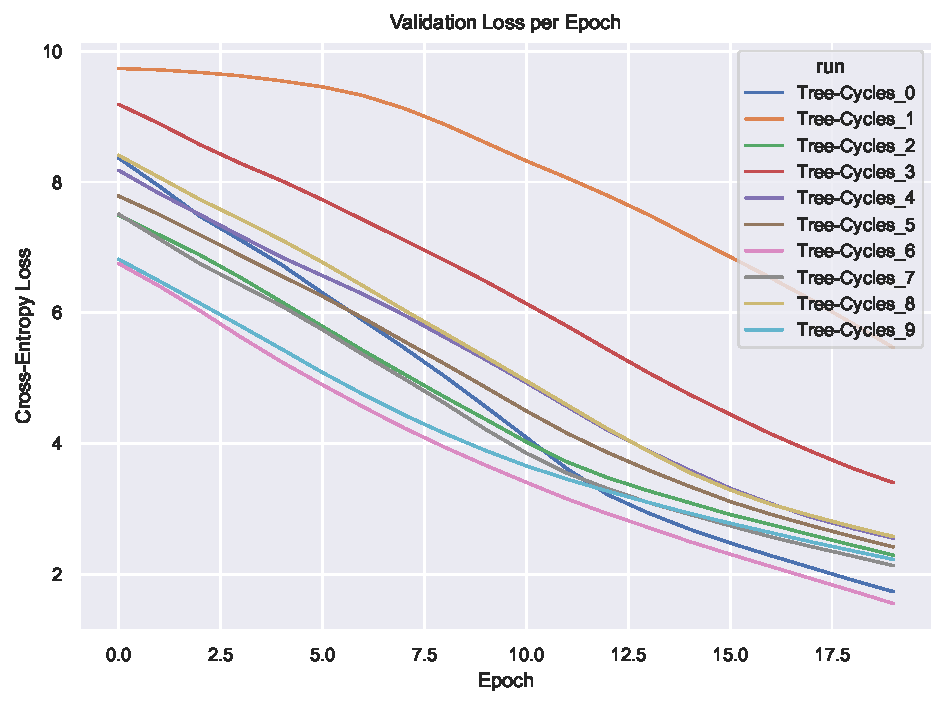
\includegraphics[width=\textwidth]{img/plots/val_loss_plot.pdf}  % Plot 1
        \caption{Mean validation Loss per Epoch (Tree-Cycles).}
        \label{fig:Tree-Cycles-val_loss}
    \end{minipage}
    \hfill
    \begin{minipage}{0.48\textwidth}
        \centering
        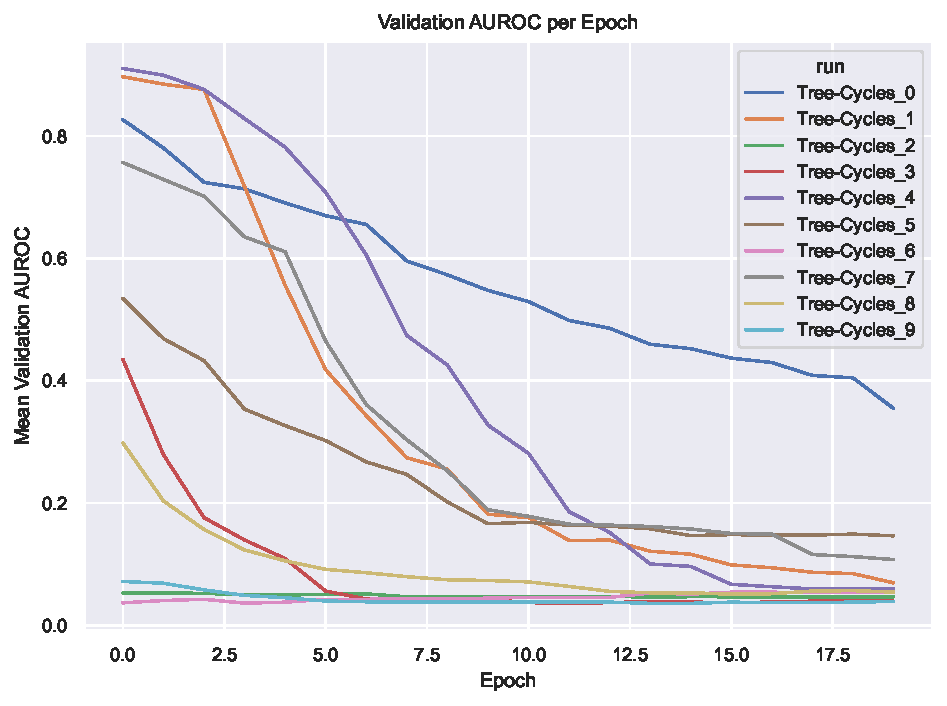
\includegraphics[width=\textwidth]{img/plots/val_auroc_plot.pdf}  % Plot 2
        \caption{Mean validation AUROC per Epoch (Tree-Cycles).}
        \label{fig:Tree-Cycles-val_auroc}
    \end{minipage}
\end{figure}

TREE-GRID DOES NOT PERFORM WELL ON METRIC IN INDUCTIVE SETTING, CLOSE TO RANDOMNESS. QUALITATIVE RESULTS HOWEVER LOOK QUITE PROMISING. RESULTS ACHIEVED IN COLLECTIVE SETTING ALSO ALMOST IDENTICAL TO THE ONES ACHIEVED IN THE REPLICATION PAPER. USAGE OF ALL MOTIF NODES LEADS TO k-HOP GRAPHS THAT DO NOT CONTAIN COMPLETE MOTIF! LEADS TO EXPLANATION ONLY CONTAINING 3 "BOXES" OF THE 4, AS SEEN IN BAD PERFORMING MODELS?
DURING OUR TRAINING: 11 of 30 training instances consisted of only motif nodes/edges, resulting in an incomputable AUROC
NOTABLE THAT LOSS DOES CONVERGE 

\begin{figure}[htbp]
    \centering
    \begin{minipage}{0.48\textwidth}
        \centering
        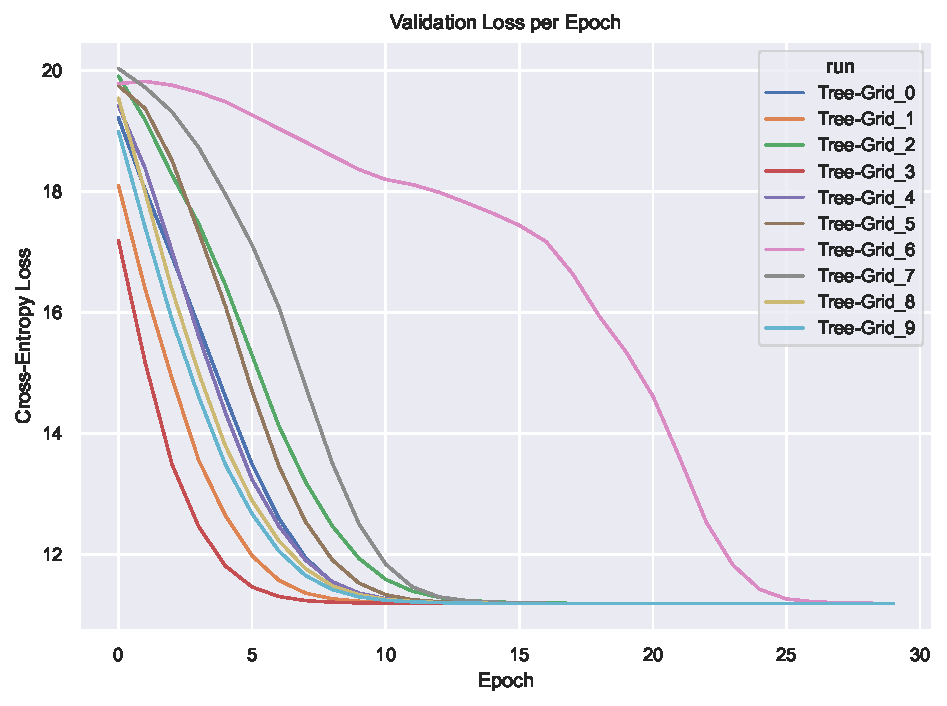
\includegraphics[width=\textwidth]{img/plots/Grid_val_loss_plot.pdf}  % Plot 1
        \caption{Mean validation Loss per Epoch (Tree-Grid).}
        \label{fig:Tree-Grid-val_loss}
    \end{minipage}
    \hfill
    \begin{minipage}{0.48\textwidth}
        \centering
        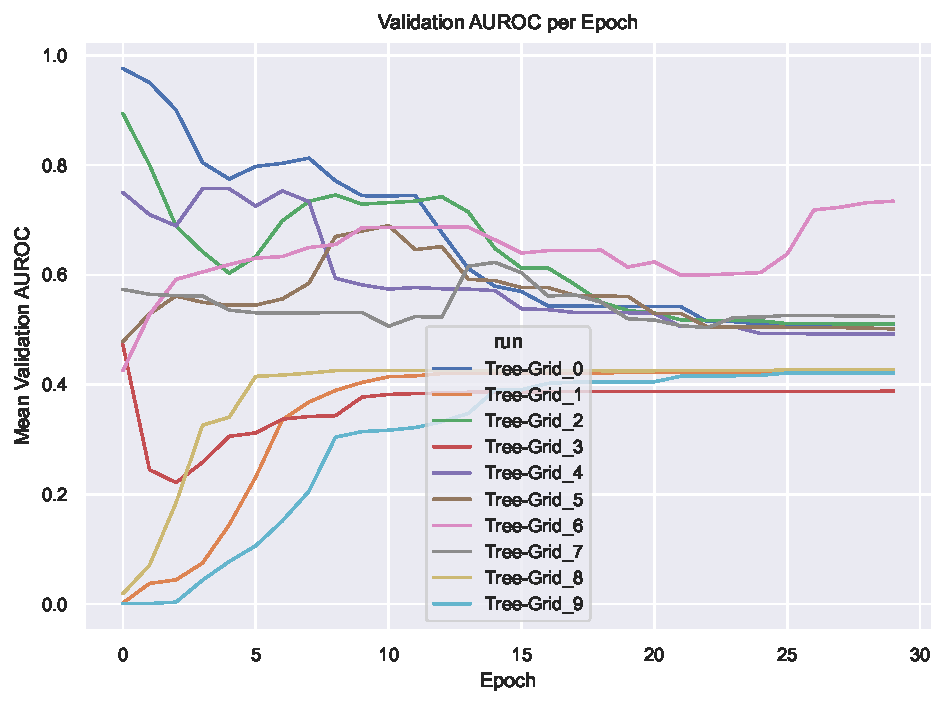
\includegraphics[width=\textwidth]{img/plots/Grid_val_auroc_plot.pdf}  % Plot 2
        \caption{Mean validation AUROC per Epoch (Tree-Grid).}
        \label{fig:Tree-Grid-val_auroc}
    \end{minipage}
\end{figure}

\begin{figure}[htbp]
    \centering
    \begin{minipage}{0.48\textwidth}
        \centering
        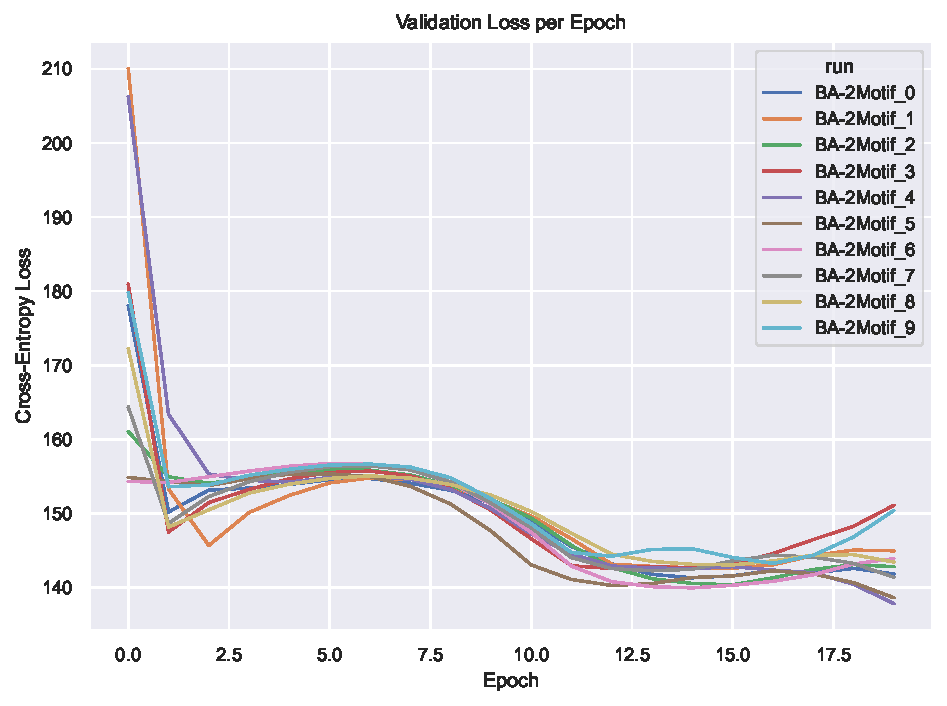
\includegraphics[width=\textwidth]{img/plots/2M_val_loss_plot.pdf}  % Plot 1
        \caption{Mean validation Loss per Epoch (BA-2Motif).}
        \label{fig:BA-2Motif-val_loss}
    \end{minipage}
    \hfill
    \begin{minipage}{0.48\textwidth}
        \centering
        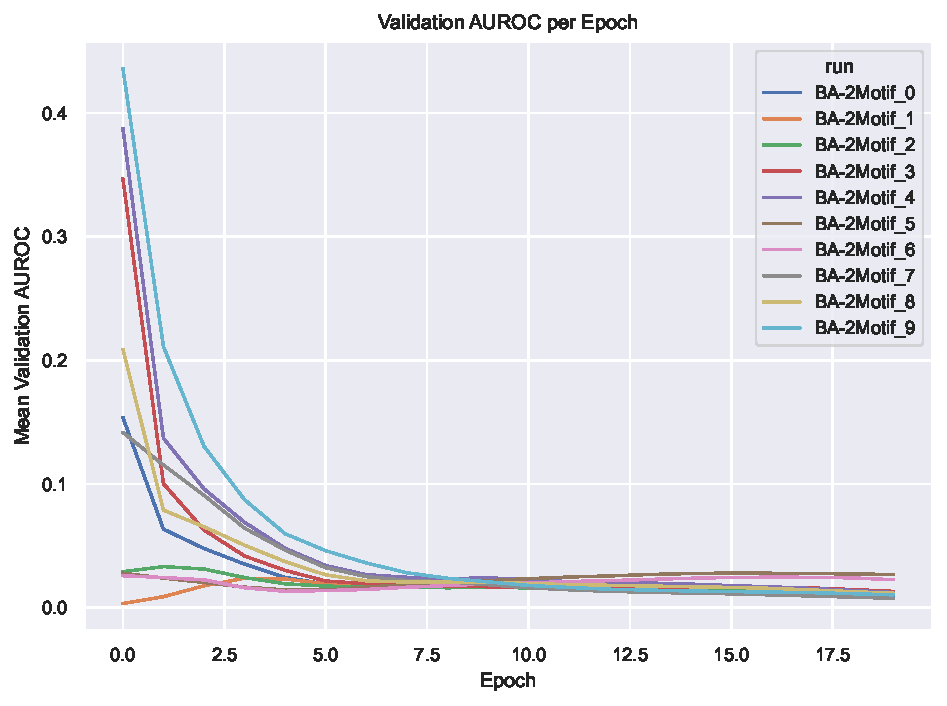
\includegraphics[width=\textwidth]{img/plots/2M_val_auroc_plot.pdf}  % Plot 2
        \caption{Mean validation AUROC per Epoch (BA-2Motif).}
        \label{fig:BA-2Motif-val_auroc}
    \end{minipage}
\end{figure}


%We use normalization in our downstream models, though it is not described in the paper, since it is used in the code. We also experimented with the effects of the use of normalization since it seems to be relevant to the performance of the explainer. \\

%It is important to highlight that our code achieved better and way more stable results for BA-2Motif when trained on a gpu instead of cpu. \\
%Ba-Shapes, Tree-Cycles and MUTAG results achieved were identical. \\
%Ba-Community and Tree-Grid achieved very slightly better results on CPU. \\

%Sweeps: (Params ordered by importance)\\
%BA-Shapes: higher size reg -> 0.1; lower entropy reg -> 0.01; lr and tT very low impact but slightly higher -> 0.01 and 5. Note that Loss curve jumps on most runs! (logical-sweep-94 and restful-sweep-92 have clean loss) TRY HIGHER SIZE REG AND LOWER ENTROPY REG \\

%BA-Community: lr 0.0001 too low, not working -> 0.003; lower entropy -> 0.1; higher size -> 0.1; TRY MORE SEEDS, LR, EPOCHS? \\

%Tree-Cycles: high lr -> 0.01 ; lower entropy reg -> 0.1/0.01; higher size reg -> 0.1/0.01 ; lower tT -> 1. TRY WITH MORE SEEDS FOR ENT, SIZE, TEMP? Confirmed higher size reg -> 0.1; lower entropy reg -> 0.01; temp really low impact, tendency higher. TRY 30 EPOCHS???\\

%Tree-Grid: high lr -> 0.01; high size reg -> 1; higher entropy reg? -> 10/1, high tT -> 5. TRY MORE SEEDS FOR ENTROPY REG -> not quite clear, tendency lower; MAYBE EVEN HIGHER LR -> No\\

%BA-2Motif: RUN ON GPU - Not the cause. Cause for better results were features of 1 instead of 0.1! However, good results achieved on BA2-Motif dataset from pyg, not original one.\\

%MUTAG: Low lr -> 0.0003; low entropy reg(high impact, but highest AUC runs vary) -> 0.1; low tT -> 1; less epochs -> 20; low size reg -> 0.005(/0.01); Loss is messy and AUC seems to decrease over time! lr 0.0001 worse, entropy reg 0.1/0.01 has zero effect -> 0.1\\


\begin{table}[ht]
    \centering
    \scriptsize
    \begin{tabularx}{\textwidth}{l*{6}{X}}   % 'X' column type from tabularx automatically scales columns
    \toprule
    \textbf{} & \multicolumn{6}{c}{\textbf{Explanation AUC}} \\
    \cmidrule{2-7}
    \textbf{Method} & BA-Shapes & BA-Community & Tree-Cycles & Tree-Grid & BA-2Motif & MUTAG \\
    \midrule
    Our work (inductive) & 0.994$\pm$0.001 & 0.754$\pm$0.013 & 0.106$\pm$0.104 & 0.537$\pm$0.081 & 0.017$\pm$0.006 & 0.874$\pm$0.009 \\
    \midrule
    with Xavier & 0.995$\pm$0.002 & 0.779$\pm$0.036 & 0.467$\pm$0.316 & 0.551$\pm$0.119 & 0.035$\pm$0.05 & 0.834$\pm$0.04 \\
    \bottomrule
    \end{tabularx}
    \caption[Inductive performance with Xavier]{PGExplainer performance in Explanation AUROC with Xavier used to initialize the Linear layer weights ($a=30$).}
    \label{tab:pgexplainer_ind_Xavier}
\end{table}


\subsection{PGExplainer in inductive setting with more training data}

\textbf{Experimental setup}
$a=60$

\textbf{Results}
\ref{tab:experiment_60train}

BA-Community: SumSampledEdges increases after 6/7 epochs, AUROC reaches peak early but then decreases steadily! (For 30 instances: Both sum sampled egdes and AUROC converge very strongly!) - Apparently less stable on 60 instances (ONLY CHANGE!!!), probably would have to be retuned (BAD!)
\begin{table}[ht]
    \centering
    \scriptsize
    \begin{tabularx}{\textwidth}{l*{6}{X}}   % 'X' column type from tabularx automatically scales columns
    \toprule
    \textbf{} & \multicolumn{6}{c}{\textbf{Explanation AUC}} \\
    \cmidrule{2-7}
    \textbf{Method} & BA-Shapes & BA-Community & Tree-Cycles & Tree-Grid & BA-2Motif & MUTAG \\
    \midrule
    Our work (inductive) & 0.994$\pm$0.001 & 0.754$\pm$0.013 & 0.106$\pm$0.104 & 0.537$\pm$0.081 & 0.017$\pm$0.006 & 0.874$\pm$0.009 \\
    \midrule
    with Xavier & 0.995$\pm$0.002 & 0.779$\pm$0.036 & 0.467$\pm$0.316 & 0.551$\pm$0.119 & 0.035$\pm$0.05 & 0.834$\pm$0.04 \\
    \midrule
    $a=60$ & 0.987.$\pm$0.002 & 0.641$\pm$0.045 & 0.144$\pm$0.096 & 0.495$\pm$0.052 & 0.017$\pm$0.004 & 0.895$\pm$0.009 \\
    \bottomrule
    \end{tabularx}
    \caption[Inductive performance with 60 training instances]{PGExplainer performance in Explanation AUROC ($a=60$) (He initialized).}
    \label{tab:experiment_60train}
\end{table}


\subsection{PGExplainer in collective setting}

\textbf{Experimental setup}
Collective setting (ALL instances used for training + testing) with hyperparameters that were found in inductive setting.

\textbf{Results}

\begin{table}[ht]
    \centering
    \scriptsize
    \begin{tabularx}{\textwidth}{l*{6}{X}}   % 'X' column type from tabularx automatically scales columns
    \toprule
    \textbf{} & \multicolumn{6}{c}{\textbf{Explanation AUC}} \\
    \cmidrule{2-7}
    \textbf{Method} & BA-Shapes & BA-Community & Tree-Cycles & Tree-Grid & BA-2Motif & MUTAG \\
    \midrule
    PGExplainer (collective) & 0.963$\pm$0.011 & 0.945$\pm$0.019 & 0.987$\pm$0.007 & 0.907$\pm$0.014 & 0.926$\pm$0.021 & 0.873$\pm$0.013 \\
    \midrule
    RE-PGExplainer (collective) & 0.999$\pm$0.000 & 0.825$\pm$0.040 & 0.760$\pm$0.014 & 0.679$\pm$0.008 & 0.133$\pm$0.046 & 0.843$\pm$0.084 \\
    \midrule
    Our work (collective) & 0.993$\pm$0.001 & 0.831$\pm$0.009 & 0.084$\pm$0.078 & 0.679$\pm$0.032 & 0.018$\pm$0.004 & 0.833$\pm$0.006 \\
    \midrule
    collective with Xavier & 0.993.$\pm$0.003 & 0.833$\pm$0.023 & 0.322$\pm$0.278 & 0.68$\pm$0.057 & 0.027$\pm$0.009 & 0.774$\pm$0.034 \\
    \midrule
    \midrule
    Our work (inductive) & 0.994$\pm$0.001 & 0.754$\pm$0.013 & 0.106$\pm$0.104 & 0.537$\pm$0.081 & 0.017$\pm$0.006 & 0.874$\pm$0.009 \\
    \bottomrule
    \end{tabularx}
    \caption[Collective performance of our reimplementation]{PGExplainer performance in Explanation AUROC in collective setting.}
    \label{tab:pgexplainer_auc}
\end{table}

\subsection{BA-2Motif with flipped GT}

He initialized

\textbf{Experimental setup}
Mean individual AUROC is calculated identical to before, but the ground truth masks of each graph are inverted, meaning that edges in the motif now carry a label of $0$ and all other edges a label of $1$. Validation loss is evaluated as well.

\textbf{Results}

\begin{table}[ht]
    \centering
    \scriptsize
    \begin{tabularx}{0.4\textwidth}{l X}
        \toprule
        \textbf{Method} & \textbf{Explanation AUC} \\
        \midrule
        Our work       & 0.017 $\pm$ 0.006 \\
        Flipped GT     & 0.985 $\pm$ 0.006 \\
        \bottomrule
    \end{tabularx}
    \caption[Inductive performance on BA-2Motif with flipped ground truth]{Explanation AUROC for BA-2Motif with flipped GT.}
    \label{tab:allmotifnodes_selected}
\end{table}

Validation Loss curve relatively smooth. TODO: INCLUDE

\subsection{Effects of motif node sets}
\label{sec:motif_set_experiment}

We conduct an experiment on the performance with only select motif nodes! only taking 30 random nodes from all motif nodes may lead to a selection of mostly nodes where not even the complete motif, and even less probable edges outside the motif, are contained.

Therefore, we change the motif nodes that are used for training/evaluating to include all or one select motif node, depending on the dataset. We use the same hyperparameters used for the previous experiments. Besides this change, we follow the experimental setup to evaluate whether a reasoning behind the node selection can be made out.

\textbf{Experimental setup}

He initialized

AllMotifNodes experiment:
BA-Shapes: All house nodes (300 nodes)
Tree-Cycles: All Cycle nodes (360 nodes)
\bigskip


OneMotifNode experiment:

BA-Community:
\begin{verbatim}
    middleCommNodes = [i for i in range(single_label.shape[0]) if single_label[i] == 1 or single_label[i] == 5]
    singularNodes = [_ for i,_ in enumerate(middleCommNodes) if i%2 == 0]
\end{verbatim}
(One of the two middle house nodes) (160 nodes)

Tree-Grid:
[512,800,9]
(One of the two nodes that connect to the base connection node for each motif, to contain full motif) (32 nodes)

Maybe works well because if all motif nodes are used, subgraphs are used where only the motif or even only part of the motif is present (Tree-Grid). Thus constantly using one singular same node that contains the complete motif may be better?


\textbf{Results}

\begin{table}[ht]
    \centering
    \scriptsize
    \begin{tabularx}{0.6\textwidth}{l*{2}{X}}   % Adjust width as needed
    \toprule
    \textbf{} & \multicolumn{2}{c}{\textbf{Explanation AUC}} \\
    \cmidrule{2-3}
    \textbf{Method} & BA-Shapes & Tree-Cycles \\
    \midrule
    Our work & 0.994$\pm$0.001 & 0.106$\pm$0.104 \\
    \midrule
    AllMotifNodes & 0.959$\pm$0.004 & 0.204$\pm$0.162 \\
    \midrule
    AllMotifNodes Xavier & 0.948$\pm$0.015 & 0.247$\pm$0.197 \\
    \bottomrule
    \end{tabularx}
    \caption[Inductive performance using all motif nodes for training]{Explanation AUROC and inference time for AllMotifNodes on selected datasets.}
    \label{tab:allmotifnodes_selected}
\end{table}

\begin{table}[ht]
    \centering
    \scriptsize
    \begin{tabularx}{0.6\textwidth}{l*{2}{X}}   % Adjust width as needed
    \toprule
    \textbf{} & \multicolumn{2}{c}{\textbf{Explanation AUC}} \\
    \cmidrule{2-3}
    \textbf{Method} & BA-Community & Tree-Grid \\
    \midrule
    Our work & 0.754$\pm$0.013 & 0.537$\pm$0.081 \\
    \midrule
    OneMotifNode & 0.951$\pm$0.007 & 1.0$\pm$0.0 \\
    \bottomrule
    \end{tabularx}
    \caption[Inductive performance using one motif node for training]{Explanation AUROC and inference time for OneMotifNode on selected datasets.}
    \label{tab:allmotifnodes_selected}
\end{table}


\subsection{Qualitative Analysis}

\textbf{Experimental setup}

Top 5 edges were taken for BA-2Motif, as done in original. This accounts for all edges of the circle motif and 5 of the 6 edges in a house motif.

For MUTAG the top 10 edges are selected, as the authors state that the shared base motif is also learned.

For Tree-Cycles and BA-2Motif the lowest AUROC models were used and the top-k lowest edges were sampled.

\textbf{Results}

We found that the MUTAG explainer detects the chemical combinations that cause the mutagenicity as the highest edge quite often, but the shared base ring is not detected at all. The explainer detects the general 2 element combinations over the rings?


%\subsection{Training on ALL instances - Evaluation only on motif instances?}
%This probably would not grant any insights, since training on non motif nodes should in theory mostly lead to all edges being irrelevant for prediction?? Bascially most edge could be removed and in theory the prediction of the node should not change at all, therefore no information can be gather from this?

%\textbf{Experimental setup}

%\textbf{Results}

\subsection{BA-2Motif with wrong features}
- Effects of using "wrong" node features for downstream task?

Comparison to orginal one: Original dataset transformed to pytorch performs way worse, for features of 0.1! Mean AUC of about 0.4! \\
Original dataset with features changed to ones instead of 0.1: Works good as well.



\section{PGExplainer applied to NeuroSAT}
\label{sec:SAT-experiments}

TODO: We present our approach for generating bipartite explanations for NeuroSAT \cite{} predictions of SAT problems.

\subsection{Common experimental setup}

We create required data with provided methods, add unsat cores and MUSs as gt


Generated batches of unsat problems that "turned" unsat because of last added clause. 10 literals per problem. Only unsat to test for unsat cores, that only apply for unsat problems. Calculated unsat cores with solver xy by adding negative assumption literals per clause and passing these as assumption for calulation. The edges of the clauses present in the unsat core were treated as ground truth. \\


For quant. eval. adapted roc auc as metric as done in PGExplainer. Results seem "good" but qual. eval. shows different result. roc auc bad metric? \\
For qual. eval. topk(=number of edges in gt) edges of predictions were highlighted to be compared to gt edges. For quant. eval. the edge probabilites were compared to gt with 1s for edges in gt and 0s for rest. \\

NeuroSAT model achieves accuracy of 1.0 on the unsat problems used.





\subsection{Soft constraint}

\textbf{Hyperparameter search}
We perform a hyperparameter search for both the explainer with the soft constraint, and the explainer with the hard constraints.

\textbf{Results}


\subsection{Hard constraint}

\textbf{Hyperparameter search}
We perform a hyperparameter search for both the explainer with the soft constraint, and the explainer with the hard constraints.
    \chapter{Discussion}

Lorem ipsum dolor sit amet, consetetur sadipscing elitr, sed diam nonumy eirmod tempor invidunt ut labore et dolore magna aliquyam erat, sed diam voluptua.



WHAT? Maybe works well because if all motif nodes are used, subgraphs are used where only the motif or even only part of the motif is present (Tree-Grid). Thus constantly using one singular same node that contains the complete motif may be better? \bigskip


\subsection{Generalizability of PGExplainer}


\subsection{Explanations for UNSAT predictions of NeuroSAT}


    \chapter{Conclusion}

To conclude this work we highlight our key findings and incentivize future work on the subject.
Though the replication of PGExplainer came with many inconsistencies and proved to be not as general as originally claimed, our results suggest that the method is able to explain instances inductively, as long as the instances used share the same topological information regarding the motifs. Generally explaining different node instances from the same motif proved to be more difficult and requires further investigation. In addition, further experiments regarding the observable flipped explanations are necessary to better understand and leverage this behavior. 
TODO: ABSTRACT SENTENCE???
In brief, our work presents the PGExplainer in a more general context, seeking to pave the way for more universal approaches to evaluating GNN explanations.

Moreover, we were able to apply the PGExplainer to a NeuroSAT model and generate bipartite explanations for unsatisfiable problems in the form of subclauses. However, these do not meet our assumption of aligning with unsatisfiable cores. 

We are optimistic that further work may allow for creating explanations that support NeuroSAT predictions.

    \cleardoublepage
    \phantomsection
    \addcontentsline{toc}{chapter}{\bibname}
    \printbibliography

    \appendix
    \chapter{Supplementary Material}

\section{Material from original PGExplainer}
\label{sec:PGE_material}
This section contains the reprinted pseudocode by Luo et al. \cite{luo2020parameterized} in algorithms \ref{alg:node-alg} and \ref{alg:graph-alg}, as well as the accuracies achieved by their used target models in Table \ref{tab:compact-accuracy}.

\begin{algorithm}
    \caption{Training Algorithm for Explaining Node Classification from \cite{luo2020parameterized}.}
    \label{alg:node-alg}
    \begin{algorithmic}[1]
    \REQUIRE Input graph $G_o = (\mathcal{V}, \mathcal{E})$, node features $X$, node labels $Y$, set of instances to be explained $\mathcal{I}$, trained GNN model: $\text{GNNE}_{\Phi_0}(\cdot)$ and $\text{GNNC}_{\Phi_1}(\cdot)$, parameterized explainer MLP $\Psi$.
    \FOR{each node $i \in \mathcal{I}$}
        \STATE $G^{(i)}_o \leftarrow$ extract the computation graph for node $i$.
        \STATE $Z^{(i)} \leftarrow \text{GNNE}_{\Phi_0}(G^{(i)}_o, X)$.
        \STATE $Y^{(i)} \leftarrow \text{GNNC}_{\Phi_1}(Z^{(i)})$.
    \ENDFOR
    \FOR{each epoch}
        \FOR{each node $i \in \mathcal{I}$}
            \STATE $\Omega \leftarrow$ latent variables calculated with (10).
            \FOR{$k \leftarrow 1$ to $K$}
                \STATE $G^{(i,k)}_s \leftarrow$ sampled from (4).
                \STATE $\hat{Y}^{(i,k)}_s \leftarrow \text{GNNC}_{\Phi_1}(\text{GNNE}_{\Phi_0}(G^{(i,k)}_s, X))$.
            \ENDFOR
        \ENDFOR
        \STATE Compute loss with (9).
        \STATE Update parameters $\Psi$ with backpropagation.
    \ENDFOR
    \end{algorithmic}
    \end{algorithm}
    
    \vspace{0.5cm}
    
    \begin{algorithm}
    \caption{Training Algorithm for Explaining Graph Classification from \cite{luo2020parameterized}.}
    \label{alg:graph-alg}
    \begin{algorithmic}[1]
    \REQUIRE A set of input graphs with $i$-th graph represented by $G^{(i)}_o$, node features $X^{(i)}$, label $Y^{(i)}$, trained GNN model: $\text{GNNE}_{\Phi_0}(\cdot)$ and $\text{GNNC}_{\Phi_1}(\cdot)$, parameterized explainer MLP $\Psi$.
    \FOR{each graph $G^{(i)}_o$}
        \STATE $Z^{(i)} \leftarrow \text{GNNE}_{\Phi_0}(G^{(i)}_o, X^{(i)})$.
        \STATE $Y^{(i)} \leftarrow \text{GNNC}_{\Phi_1}(Z^{(i)})$.
    \ENDFOR
    \FOR{each epoch}
        \FOR{each graph $G^{(i)}_o$}
            \STATE $\Omega \leftarrow$ latent variables calculated with (11).
            \FOR{$k \leftarrow 1$ to $K$}
                \STATE $G^{(i,k)}_s \leftarrow$ sampled from (4).
                \STATE $\hat{Y}^{(i,k)}_s \leftarrow \text{GNNC}_{\Phi_1}(\text{GNNE}_{\Phi_0}(G^{(i,k)}_s, X^{(i)}))$.
            \ENDFOR
        \ENDFOR
        \STATE Compute loss with (9).
        \STATE Update parameters $\Psi$ with backpropagation.
    \ENDFOR
    \end{algorithmic}
\end{algorithm}

\begin{table}[h]
    \centering
    \scriptsize
    \begin{tabularx}{\linewidth}{l|X X X X|X X}
    \hline
    \textbf{Accuracy} & \textbf{BA-Shapes} & \textbf{BA-Community} & \textbf{Tree-Cycles} & \textbf{Tree-Grid} & \textbf{BA-2Motif} & \textbf{MUTAG} \\
    \hline
    \textbf{Training}   & 0.98 & 0.99 & 0.99 & 0.92 & 1.00 & 0.87 \\
    \textbf{Validation} & 1.00 & 0.88 & 1.00 & 0.94 & 1.00 & 0.89 \\
    \textbf{Testing}    & 0.97 & 0.93 & 0.99 & 0.94 & 1.00 & 0.87 \\
    \hline
    \end{tabularx}
    \caption[Accuracies of original GNN downstream task]{Compact accuracy table for Node and Graph Classification. Reprinted from \cite{luo2020parameterized}.}
    \label{tab:compact-accuracy}
\end{table}


\section{Data visualization}
\label{sec:data_vis}

\begin{figure}[H]
    \centering
    \begin{subfigure}[b]{0.4\textwidth}
        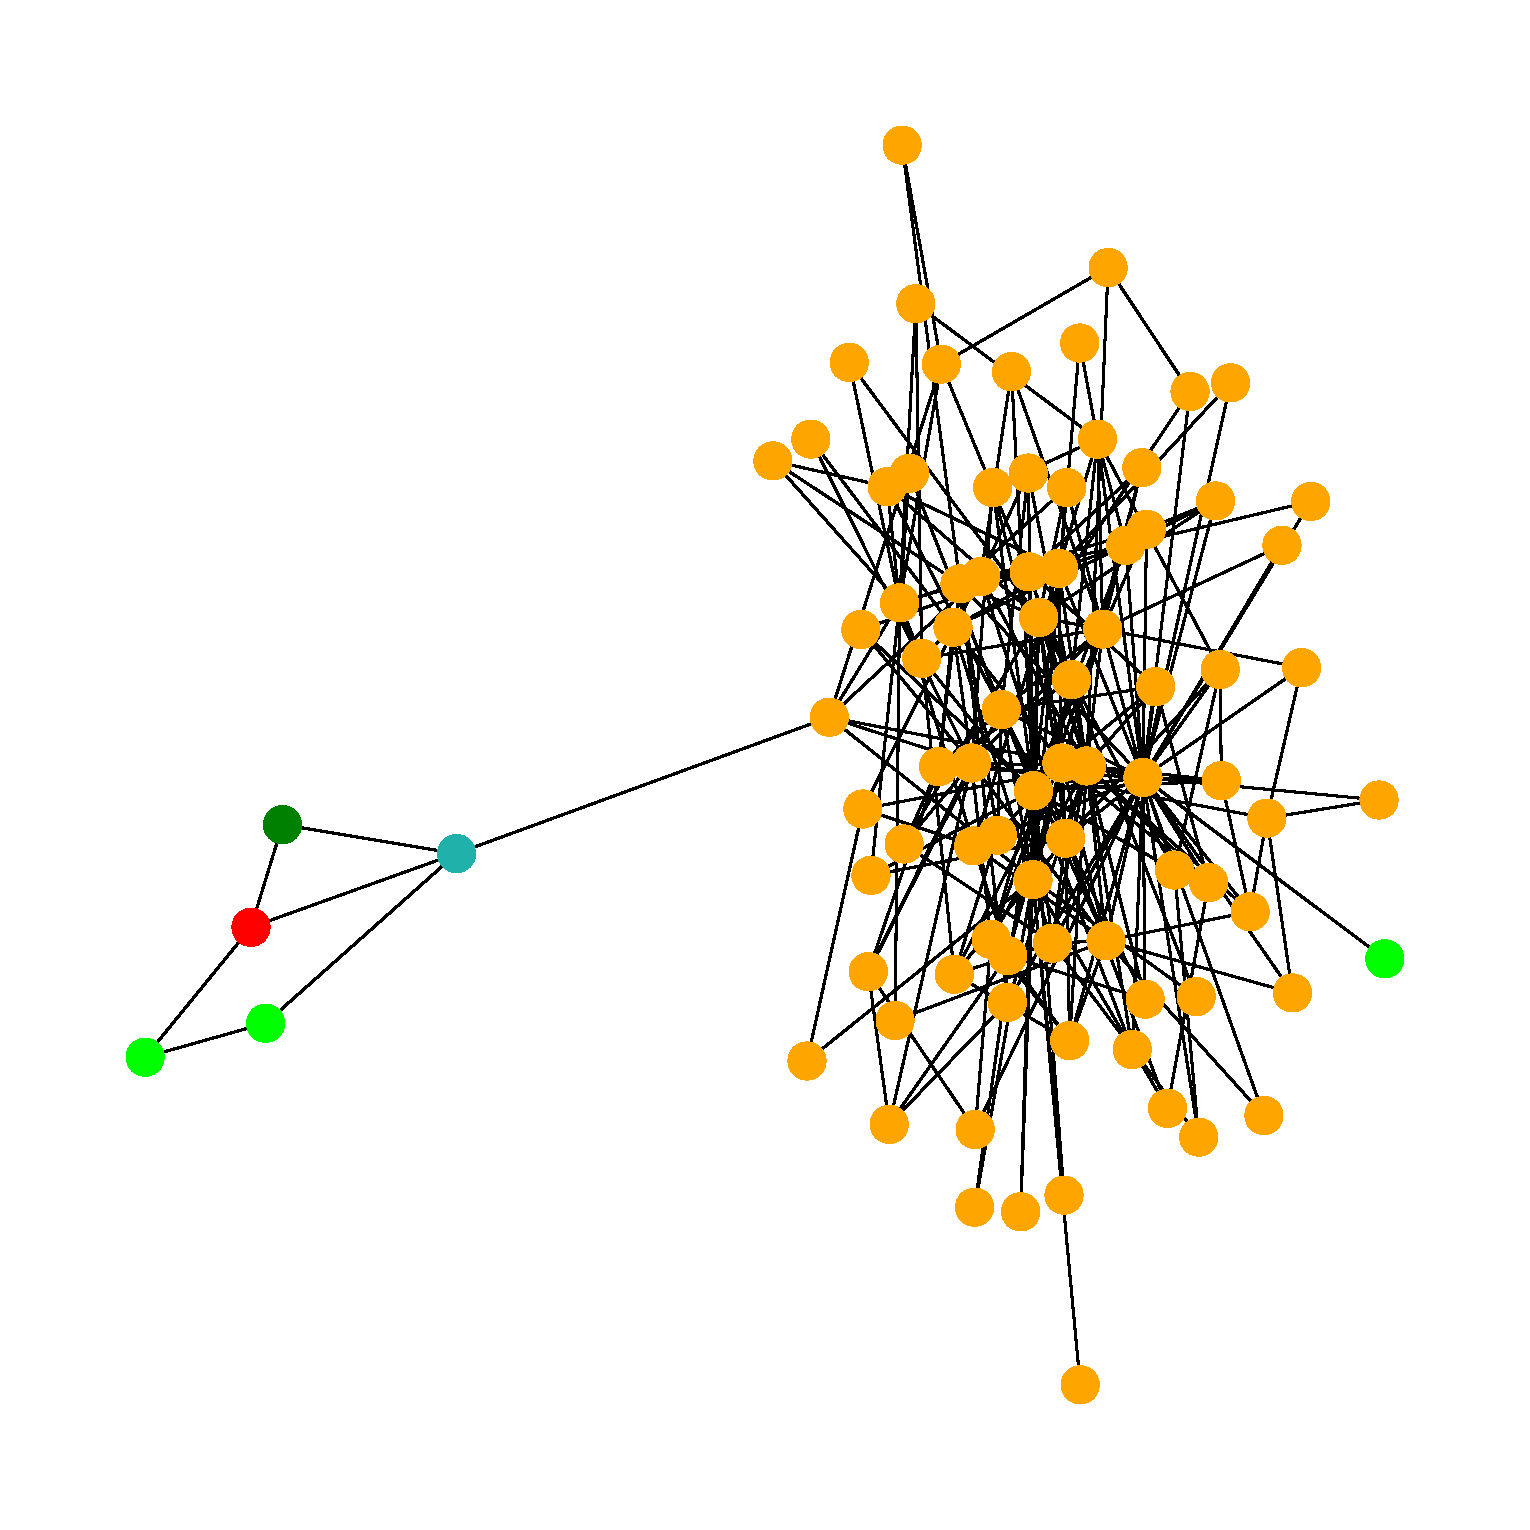
\includegraphics[width=\textwidth]{img/BA-Shapes-VIS-COMP-GRAPH.pdf}
        \caption{BA-Shapes}
    \end{subfigure}
    \hfill
    \begin{subfigure}[b]{0.4\textwidth}
        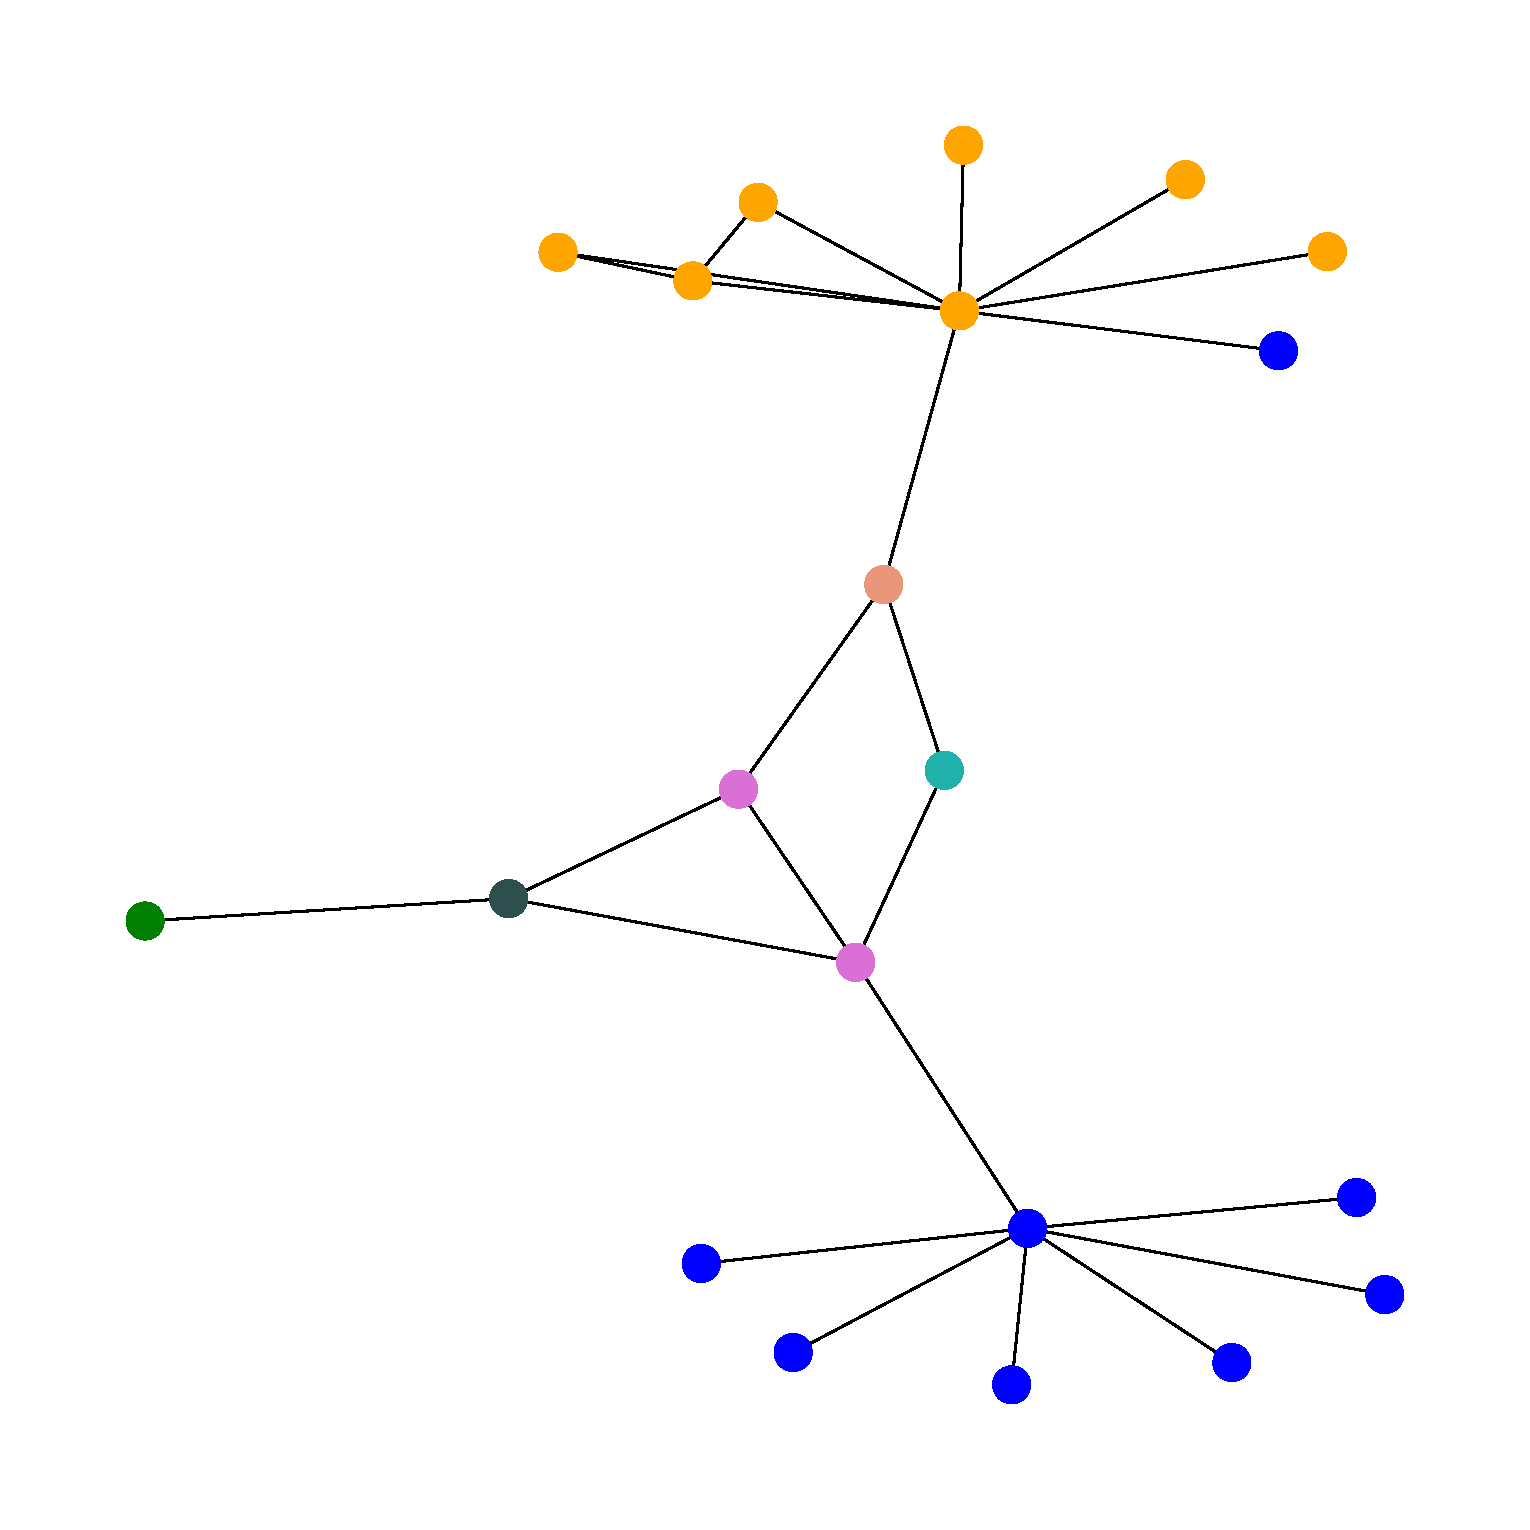
\includegraphics[width=\textwidth]{img/BA-Community-VIS-COMP-GRAPH.pdf}
        \caption{BA-Community}
    \end{subfigure}
    
    \vspace{0.5cm}
    
    \begin{subfigure}[b]{0.4\textwidth}
        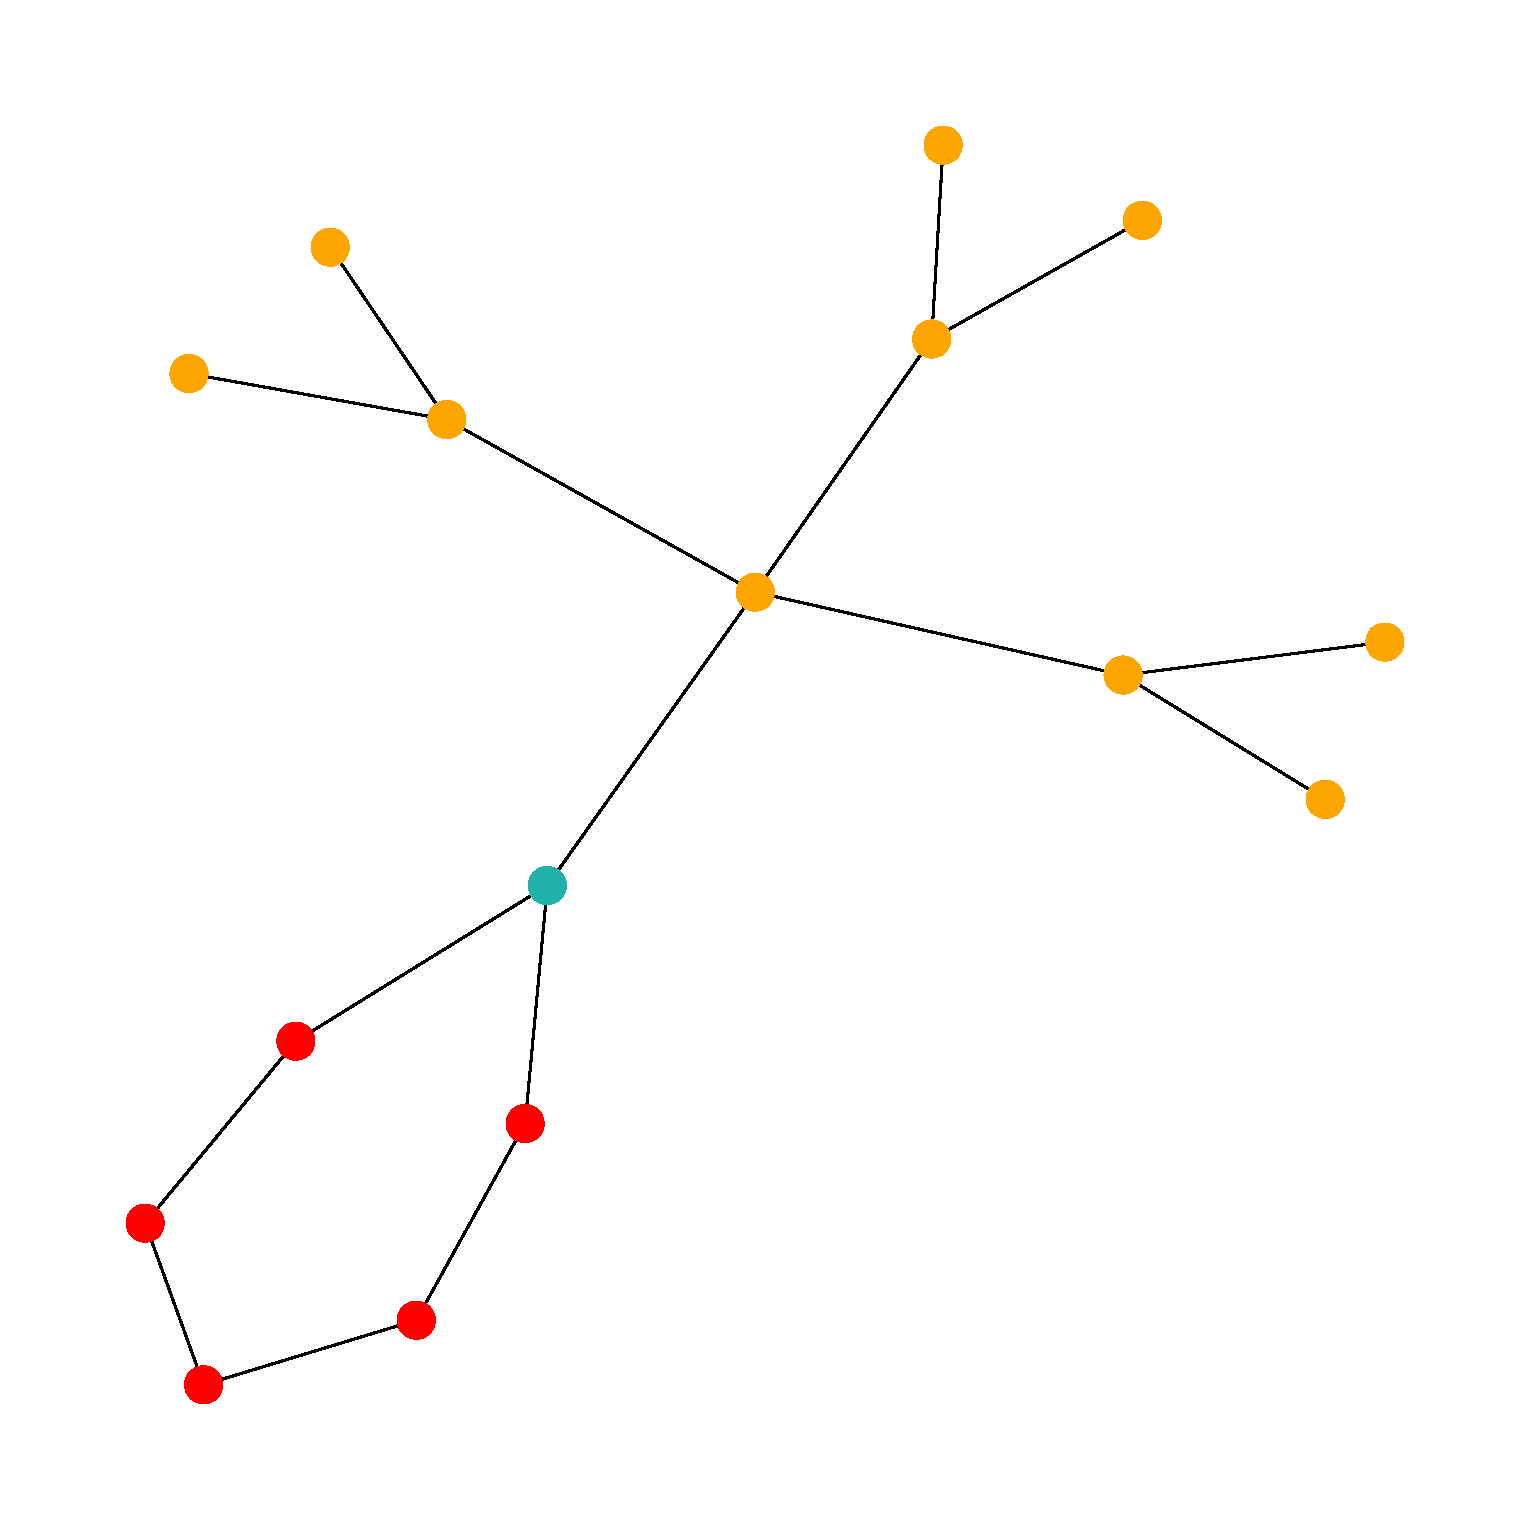
\includegraphics[width=\textwidth]{img/Tree-Cycles-VIS-COMP-GRAPH.pdf}
        \caption{Tree-Cycles}
    \end{subfigure}
    \hfill
    \begin{subfigure}[b]{0.4\textwidth}
        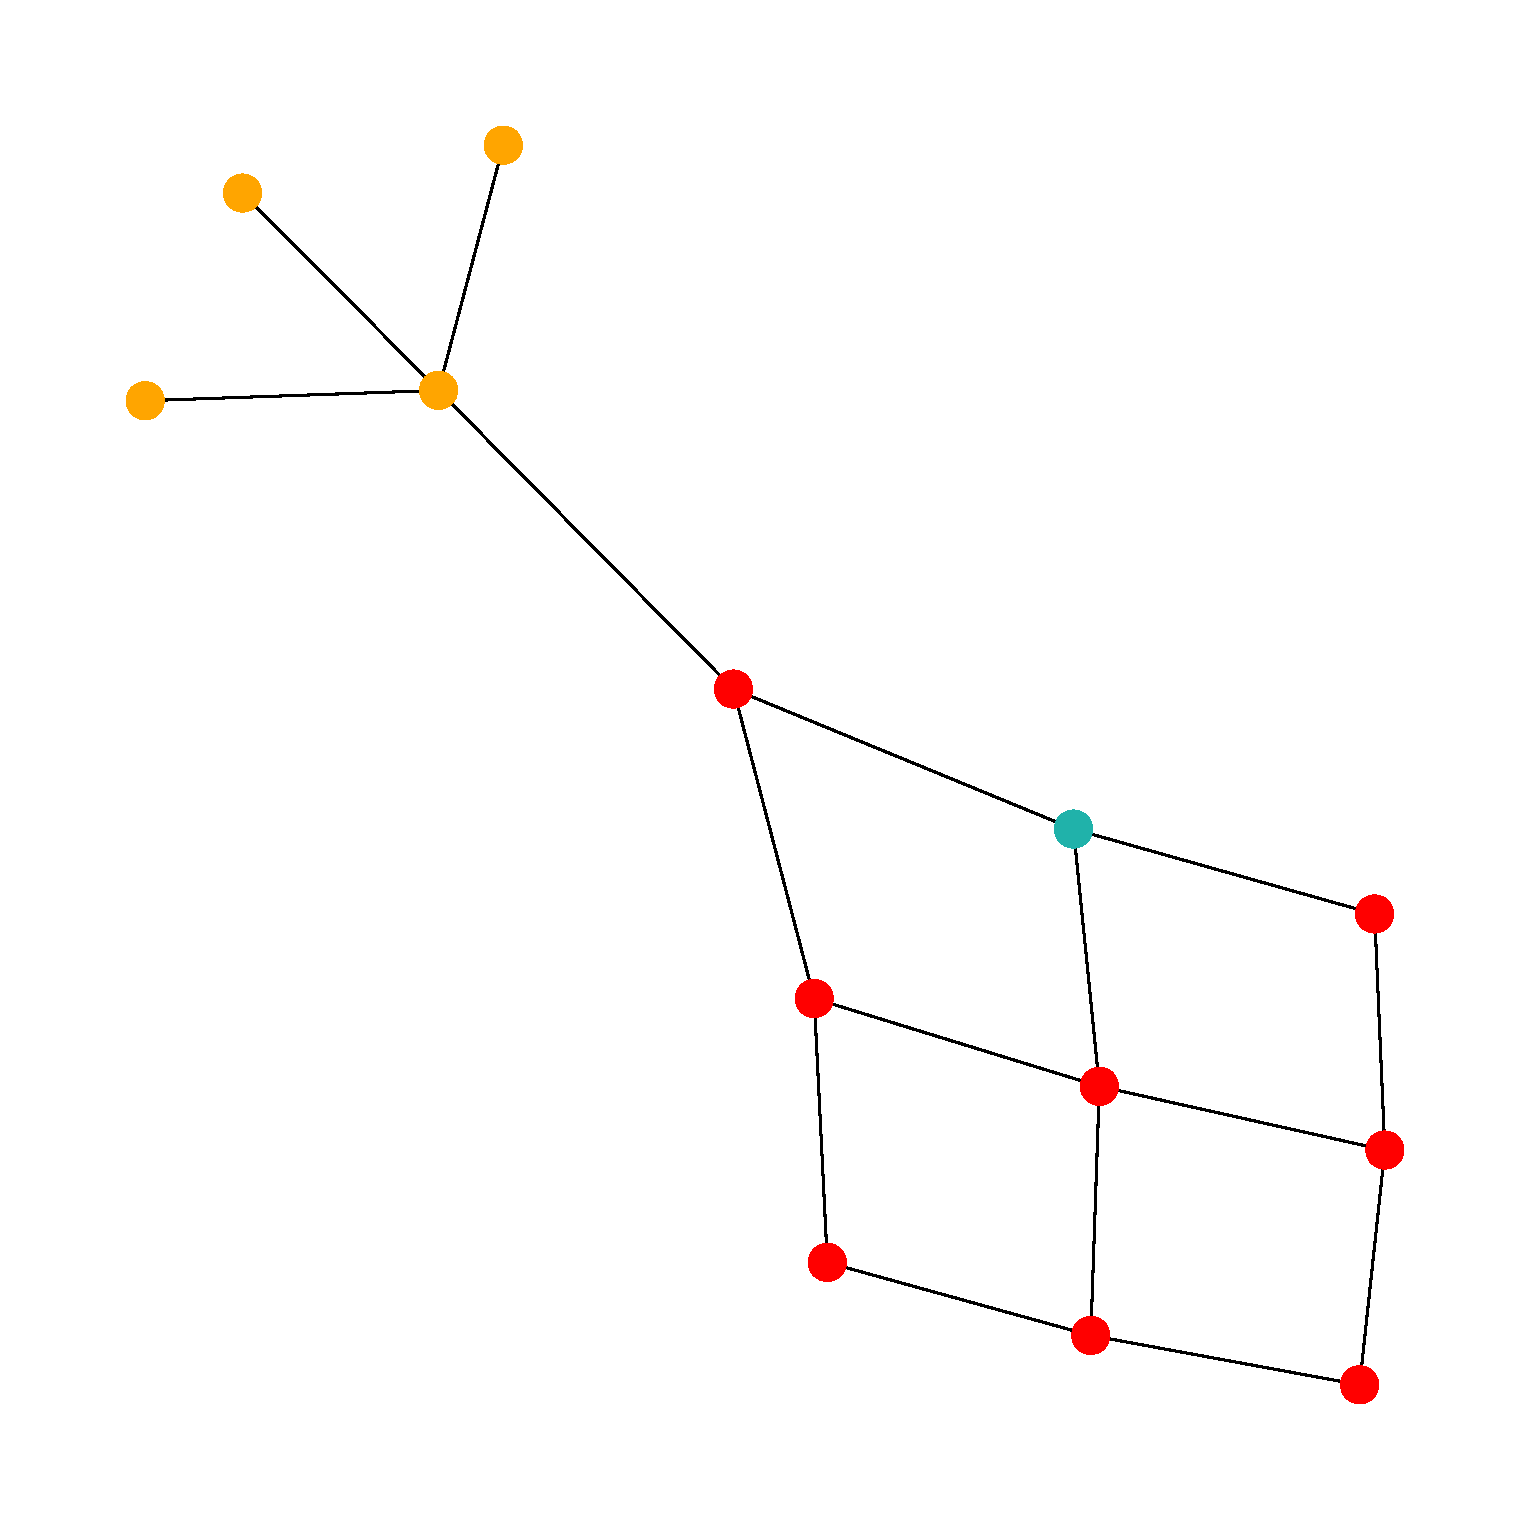
\includegraphics[width=\textwidth]{img/Tree-Grid-VIS-COMP-GRAPH.pdf}
        \caption{Tree-Grid}
    \end{subfigure}
    
    \vspace{0.5cm}
    
    \begin{subfigure}[b]{0.4\textwidth}
        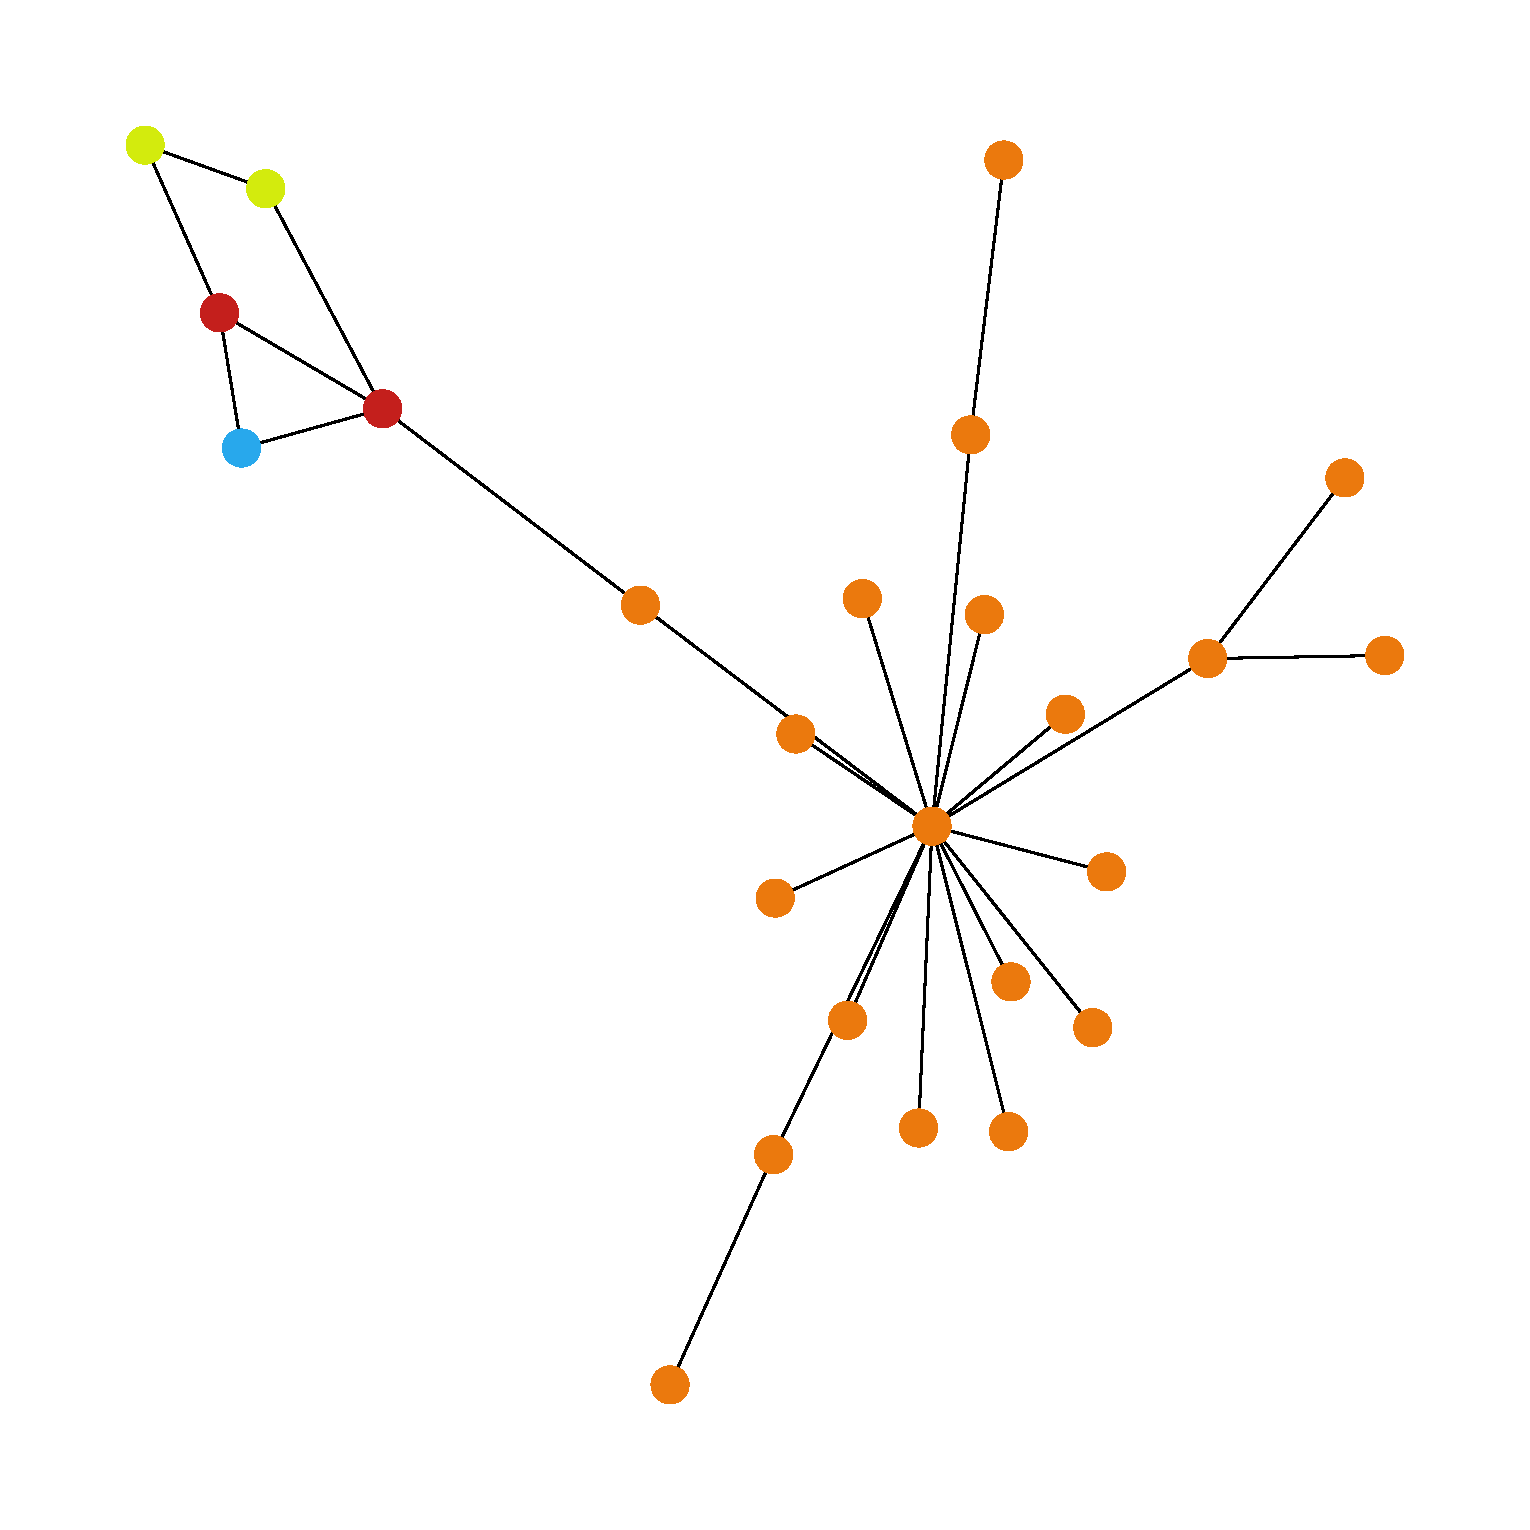
\includegraphics[width=\textwidth]{img/BA-2Motif-VIS-UNLABELED.pdf}
        \caption{BA-2Motif}
    \end{subfigure}
    \hfill
    \begin{subfigure}[b]{0.4\textwidth}
        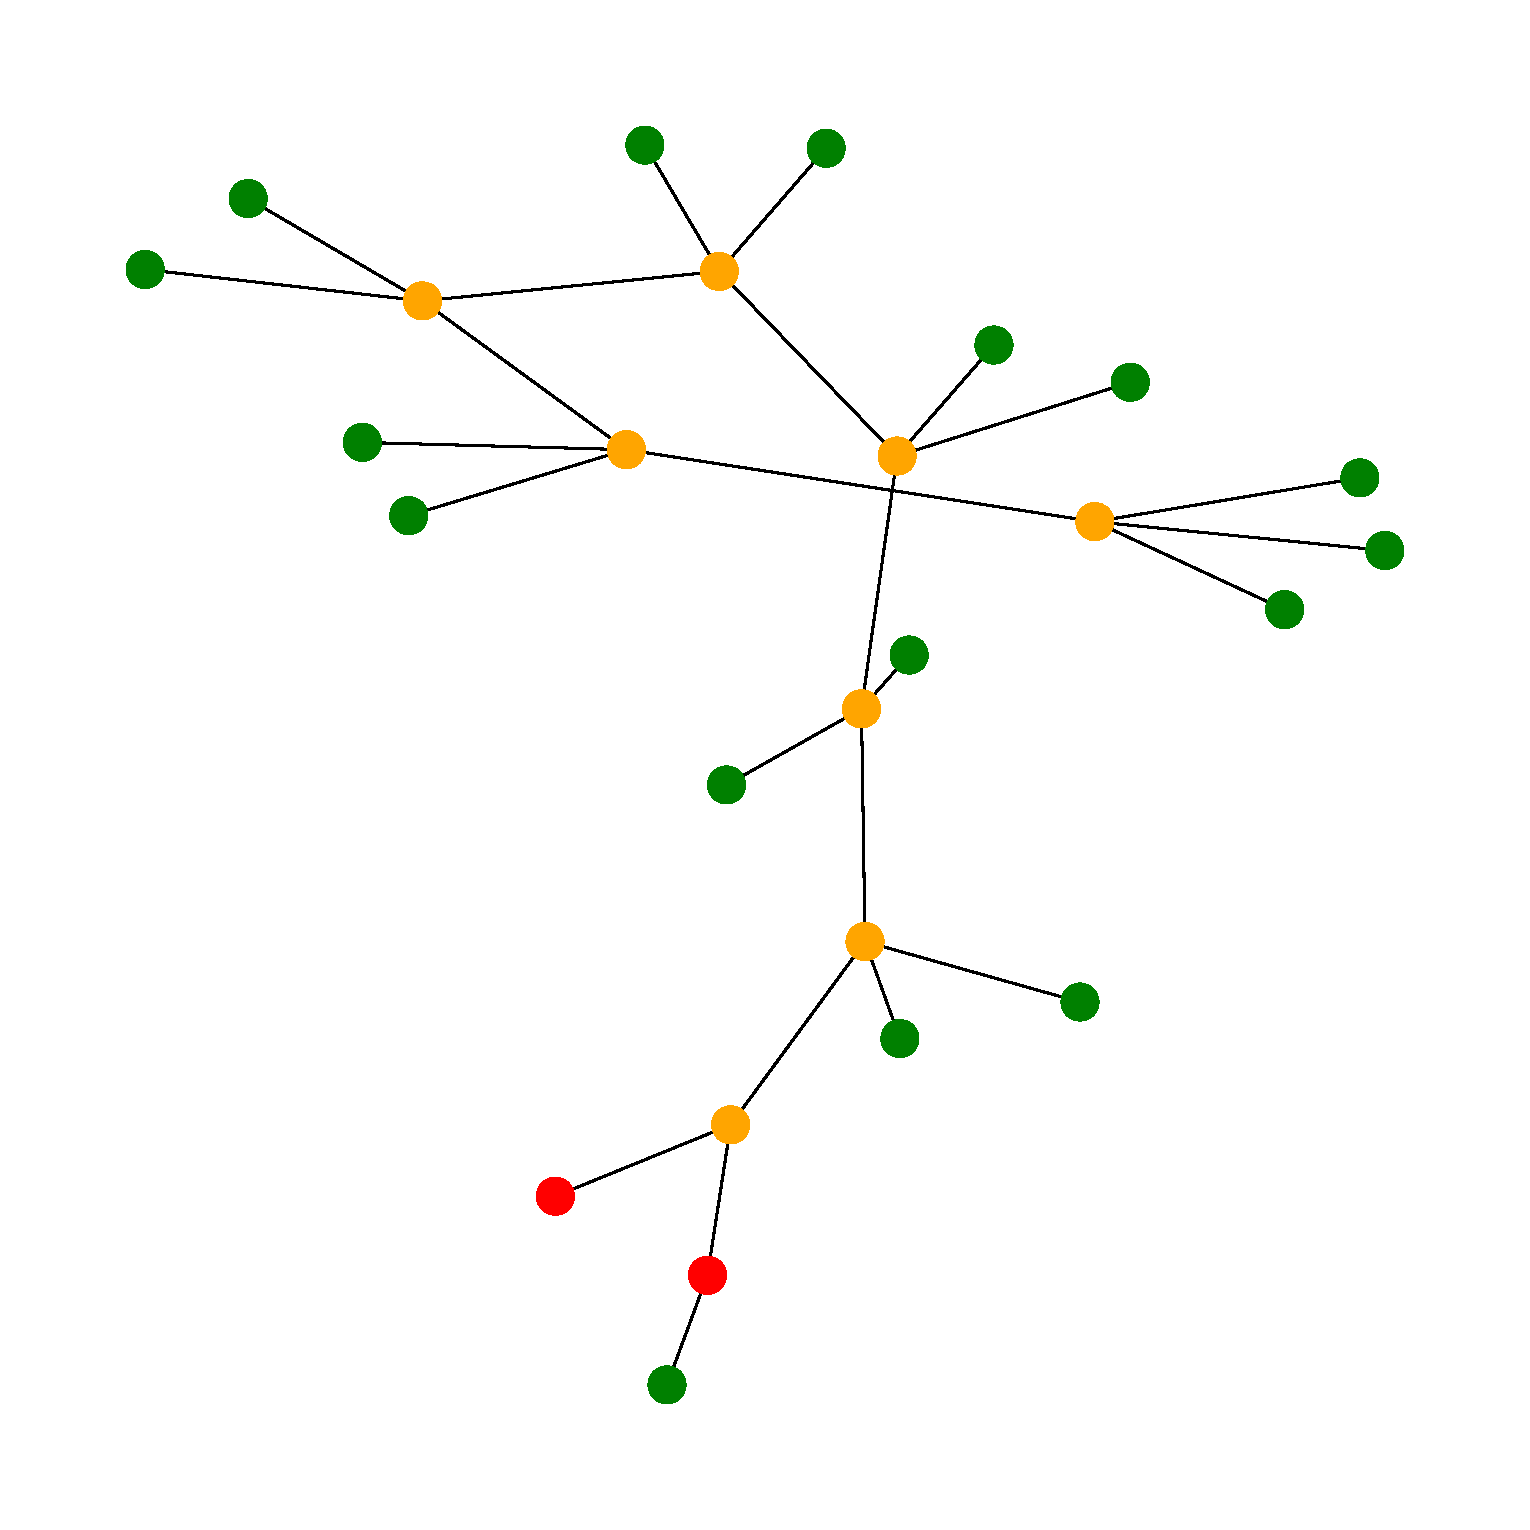
\includegraphics[width=\textwidth]{img/MUTAG-VIS-LARGE-UNLABELED.pdf}
        \caption{MUTAG}
    \end{subfigure}

    \caption[Visualization of original PGExplainer datasets]{Visualization of all six datasets. For node datasets (a-d) the target prediction node where the computational graph is computed from is colored in light blue.}
\end{figure}

\section{Replication Hyperparameter Searches}
\label{sec:sweeps}
The following tables contain the grid search configurations for the explainer on each target model. The first row includes the configuration used in the original codebase \cite{luo2020parameterized} and the second row contains the configurations used in \cite{holdijk2021re}. For BA-Community (see Table \ref{tab:BA-Community_sweep}) both configurations are identical, and the second row is thus omitted. The last section of each table contains the set of the values that we tested for each parameter. The optimal settings for our explainer implementation are highlighted in each column. Note that we optimize Tree-Cycles (see Table \ref{tab:Tree-Cycles_sweep}) and BA-2Motif (see Table \ref{tab:BA-2M-sweep}) towards a minimal metric score, as discussed in Section \ref{sec:ind_results}.

\newcolumntype{Y}{>{\centering\arraybackslash}X}
\begin{table}[h]
  \centering
  \scriptsize
  \begin{tabular}{|c|c|c|c|c|c|c|c|c|c|}
  \hline
  \multicolumn{10}{|c|}{\textbf{BA-Shapes}} \\ \hline
  $a$ & $K$ & $b$ & $E$ & $\eta$ & $S$ & $\alpha_e$ & $\alpha_s$ & $\tau_0$ & $\tau_T$ \\ \hline
  $N$ & 1 & 0.0 & 10 & 0.003 & - & 1.0 & 0.05 & 1.0 & 0.05 \\ \hline
  $N$ & 1 & 0.0 & 10 & 0.003 & - & 1.0 & 0.05 & 5.0 & 2.0 \\ \hline
  5 & \textbf{1} & 0.0 & 10 & 0.0003 & 74 & \textbf{0.1} & 0.005 & 5.0 & \textbf{1} \\
   & 5 &  &  & \textbf{0.003} & 75 & 0.5 & \textbf{0.05} &  & 2 \\
   & 10 &  &  & 0.03 & 76 & 1.0 & 0.1 &  & 5 \\ \hline
  \end{tabular}
  \caption[BA-Shapes grid search]{First two rows show hyperparameter settings used in \cite{luo2020parameterized} and \cite{holdijk2021re}, respectively. Last section contains our grid search configuration. Bolded values indicate the best performance.}
\end{table}

\begin{table}[h]
  \centering
  \scriptsize
  \begin{tabular}{|c|c|c|c|c|c|c|c|c|c|}
  \hline
  \multicolumn{10}{|c|}{\textbf{BA-Community}} \\ \hline
  $a$ & $K$ & $b$ & $E$ & $\eta$ & $S$ & $\alpha_e$ & $\alpha_s$ & $\tau_0$ & $\tau_T$ \\ \hline
  $N$ & 1 & 0.5 & 20 & 0.003 & - & 1.0 & 0.05 & 1.0 & 1.0 \\ \hline
  64 & 1 & \textbf{0.0} & 20 & \textbf{0.003} & 74 & \textbf{1.0} & 0.05 & 1.0 & 1.0 \\
   & \textbf{5} & 0.5 &  & 0.0003 & 75 & 0.1 & \textbf{0.1} &  & \textbf{5.0} \\
   & 10 &  &  &  & 76 &  &  &  &  \\ \hline
  \end{tabular}
  \caption[BA-Community grid search]{First row shows hyperparameter settings used in \cite{luo2020parameterized} and \cite{holdijk2021re}. Last section contains our grid search configuration. Bolded values indicate the best performance.}
  \label{tab:BA-Community_sweep}
\end{table}

\begin{table}[h]
  \centering
  \scriptsize
  \begin{tabular}{|c|c|c|c|c|c|c|c|c|c|}
  \hline
  \multicolumn{10}{|c|}{\textbf{Tree-Cycles}} \\ \hline
  $a$ & $K$ & $b$ & $E$ & $\eta$ & $S$ & $\alpha_e$ & $\alpha_s$ & $\tau_0$ & $\tau_T$ \\ \hline
  $N$ & 1 & 0.0 & 20 & 0.003 & - & 0.01 & 0.0001 & 5.0 & 5.0 \\ \hline
  $N$ & 1 & 0.0 & 20 & 0.003 & - & 10.0 & 0.1 & 1.0 & 5.0 \\ \midrule
  5 & 1 & 0.0 & 20 & \textbf{0.0003} & 74 & 0.01 & \textbf{0.0001} & 1.0 & \textbf{1.0} \\
   & \textbf{5} &  &  & 0.003 & 75 & \textbf{1.0} & 0.05 &  & 5.0 \\
   & 10 &  &  &  & 76 & 10.0 & 0.1 &  &  \\ \hline
  \end{tabular}
  \caption[Tree-Cycles grid search]{First two rows show hyperparameter settings used in \cite{luo2020parameterized} and \cite{holdijk2021re}, respectively. Last section contains our grid search configuration. Bolded values indicate the best performance.}
  \label{tab:Tree-Cycles_sweep}
\end{table}

\begin{table}[h]
  \centering
  \scriptsize
  \begin{tabular}{|c|c|c|c|c|c|c|c|c|c|}
  \hline
  \multicolumn{10}{|c|}{\textbf{Tree-Grid}} \\ \hline
  $a$ & $K$ & $b$ & $E$ & $\eta$ & $S$ & $\alpha_e$ & $\alpha_s$ & $\tau_0$ & $\tau_T$ \\ \hline
  $N$ & 1 & 0.0 & 30 & 0.01 & - & 1.0 & 0.01 & 5.0 & 5.0 \\ \hline
  $N$ & 1 & 0.0 & 30 & 0.003 & - & 1.0 & 1.0 & 5.0 & 2.0 \\ \midrule
  24 & 1 & 0.0 & 30 & 0.0003 & 74 & 0.1 & 0.01 & 5.0 & \textbf{2.0} \\
   & \textbf{5} &  & 30 & \textbf{0.003} & 75 & \textbf{1.0} & \textbf{0.5} &  & 5.0 \\
   & 10 &  & 30 & 0.01 & 76 & 10 & 1.0 &  &  \\ 
   &  &  &  & 0.05 &  &  &  &  &  \\ \hline
  \end{tabular}
  \caption[Tree-Grid grid search]{First two rows show hyperparameter settings used in \cite{luo2020parameterized} and \cite{holdijk2021re}, respectively. Last section contains our grid search configuration. Bolded values indicate the best performance.}
\end{table}

\begin{table}[h]
  \centering
  \scriptsize
  \begin{tabular}{|c|c|c|c|c|c|c|c|c|c|}
  \hline
  \multicolumn{10}{|c|}{\textbf{BA-2Motif}} \\ \hline
  $a$ & $K$ & $b$ & $E$ & $\eta$ & $S$ & $\alpha_e$ & $\alpha_s$ & $\tau_0$ & $\tau_T$ \\ \hline
  $N$ & 1 & 0.0 & 10 & 0.003 & - & 0.0 & 0.00 & 1.0 & 0.0 \\ \hline
  $N$ & 1 & 0.0 & 20 & 0.005 & - & 0.01 & 0.03 & 5.0 & 1.0 \\ \midrule
  30 & 1 & 0.0 & 10 & 0.0003 & 74 & 0.01 & 0.03 & 5.0 & \textbf{1.0} \\
   & 5 &  & \textbf{20} & 0.003 & 75 & \textbf{0.1} &  &  & 5.0 \\
   & \textbf{10} &  &  & 0.005 & 76 &  &  &  &  \\
   &  &  &  & \textbf{0.01} &  &  &  &  &  \\ \hline
  \end{tabular}
  \caption[BA-2Motif grid search]{First two rows show hyperparameter settings used in \cite{luo2020parameterized} and \cite{holdijk2021re}, respectively. Last section contains our grid search configuration. Bolded values indicate the best performance.}
  \label{tab:BA-2M-sweep}
\end{table}

\begin{table}[h]
  \centering
  \scriptsize
  \begin{tabular}{|c|c|c|c|c|c|c|c|c|c|}
  \hline
  \multicolumn{10}{|c|}{\textbf{MUTAG}} \\ \hline
  $a$ & $K$ & $b$ & $E$ & $\eta$ & $S$ & $\alpha_e$ & $\alpha_s$ & $\tau_0$ & $\tau_T$ \\ \hline
  $N$ & 1 & 0.0 & 10 & 0.01 & - & 1.0 & 0.01 & 5.0 & 5.0 \\ \hline
  $N$ & 1 & 0.0 & 30 & 0.0003 & - & 1.0 & 0.005 & 5.0 & 5.0 \\ \midrule
  30 & 1 & 0.0 & 10 & 0.0003 & 74 & 0.1 & 0.01 & 5.0 & \textbf{1.0} \\
   & 5 &  & \textbf{20} & 0.003 & 75 & \textbf{1.0} & \textbf{0.005} &  & 5.0 \\
   & \textbf{10} &  & 30 & \textbf{0.01} & 76 &  &  &  &  \\ \hline
  \end{tabular}
  \caption[MUTAG grid search]{First two rows show hyperparameter settings used in \cite{luo2020parameterized} and \cite{holdijk2021re}, respectively. Last section contains our grid search configuration. Bolded values indicate the best performance.}
\end{table}

\clearpage
\section{Multiple Explanation Visualizations}
\label{sec:grid_vis}
The following figures \ref{fig:grid-BA-Shapes-explanations}, \ref{fig:grid-BA-Community-explanations}, \ref{fig:grid-Tree-Cycles-explanations}, \ref{fig:grid-Tree-Grid-explanations}, \ref{fig:grid-BA-2Motif-explanations}, \ref{fig:grid-MUTAG-explanations} contain 16 randomly sampled explanations for the best explainer model of every dataset. For graph tasks all nodes of the input graph are included, while for node tasks only the nodes of the local computation graph from the prediction motif node are shown.

% REMOVE draw=black TO REMOVE EDGES
\begin{figure}[htbp]
    \centering
    \begin{tikzpicture}
      % 4x4 grid: row = 0 to 3, col = 0 to 3
      \foreach \row in {0,...,3} {
        \foreach \col in {0,...,3} {
          \pgfmathtruncatemacro{\num}{\col + 4 * \row}
          \node[draw=black, thin, inner sep=0pt] at (\col*4, -\row*4)
            {\includegraphics[width=3.5cm]{img/BA-Shapes/graph_\num_explanation.pdf}};
        }
      }
    \end{tikzpicture}
    \caption{Grid of BA-Shapes explanations (top-6 edges)}
    \label{fig:grid-BA-Shapes-explanations}
\end{figure}

\begin{figure}[htbp]
    \centering
    \begin{tikzpicture}
      % 4x4 grid: row = 0 to 3, col = 0 to 3
      \foreach \row in {0,...,3} {
        \foreach \col in {0,...,3} {
          \pgfmathtruncatemacro{\num}{\col + 4 * \row}
          \node[draw=black, thin, inner sep=0pt] at (\col*4, -\row*4)
            {\includegraphics[width=3.5cm]{img/BA-Community/graph_\num_explanation.pdf}};
        }
      }
    \end{tikzpicture}
    \caption{Grid of BA-Community explanations (top-6 edges)}
    \label{fig:grid-BA-Community-explanations}
\end{figure}

\begin{figure}[htbp]
    \centering
    \begin{tikzpicture}
      % 4x4 grid: row = 0 to 3, col = 0 to 3
      \foreach \row in {0,...,3} {
        \foreach \col in {0,...,3} {
          \pgfmathtruncatemacro{\num}{\col + 4 * \row}
          \node[draw=black, thin, inner sep=0pt] at (\col*4, -\row*4)
            {\includegraphics[width=3.5cm]{img/Tree-Cycles/graph_\num_explanation.pdf}};
        }
      }
    \end{tikzpicture}
    \caption{Grid of Tree-Cycles explanations (top-6 edges)}
    \label{fig:grid-Tree-Cycles-explanations}
\end{figure}

\begin{figure}[htbp]
    \centering
    \begin{tikzpicture}
      % 4x4 grid: row = 0 to 3, col = 0 to 3
      \foreach \row in {0,...,3} {
        \foreach \col in {0,...,3} {
          \pgfmathtruncatemacro{\num}{\col + 4 * \row}
          \node[draw=black, thin, inner sep=0pt] at (\col*4, -\row*4)
            {\includegraphics[width=3.5cm]{img/Tree-Grid/graph_\num_explanation.pdf}};
        }
      }
    \end{tikzpicture}
    \caption{Grid of Tree-Grid explanations (top-12 edges)}
    \label{fig:grid-Tree-Grid-explanations}
\end{figure}

\begin{figure}[htbp]
    \centering
    \begin{tikzpicture}
      % 4x4 grid: row = 0 to 3, col = 0 to 3
      \foreach \row in {0,...,3} {
        \foreach \col in {0,...,3} {
          \pgfmathtruncatemacro{\num}{\col + 4 * \row}
          \node[draw=black, thin, inner sep=0pt] at (\col*4, -\row*4)
            {\includegraphics[width=3.5cm]{img/BA-2Motif/graph_\num_explanation.pdf}};
        }
      }
    \end{tikzpicture}
    \caption{Grid of BA-2Motif explanations (top-5 edges)}
    \label{fig:grid-BA-2Motif-explanations}
\end{figure}

\begin{figure}[htbp]
    \centering
    \begin{tikzpicture}
      % 4x4 grid: row = 0 to 3, col = 0 to 3
      \foreach \row in {0,...,3} {
        \foreach \col in {0,...,3} {
          \pgfmathtruncatemacro{\num}{\col + 4 * \row}
          \node[draw=black, thin, inner sep=0pt] at (\col*4, -\row*4)
            {\includegraphics[width=3.5cm]{img/MUTAG/graph_\num_explanation.pdf}};
        }
      }
    \end{tikzpicture}
    \caption{Grid of MUTAG explanations (top-10 edges)}
    \label{fig:grid-MUTAG-explanations}
\end{figure}

\clearpage
\section{NeuroSAT explainer Hyperparameter Searches}
\label{sec:neurSAT_sweeps}

The following tables contain the grid search configurations for the NeuroSAT explainer models with either the soft constraint (see Table \ref{tab:sweep_conf_soft}) or the hard constraint (see Table \ref{tab:sweep_conf_hard}) applied. The columns contain the values tested for the corresponding hyperparameter. The optimal settings for each explainer implementation are highlighted. Figure \ref{fig:soft-sweep} shows the AUROC range of all runs performed in the grid search for the soft constraint explainer.

\begin{table}[h]
  \centering
  \scriptsize
  \begin{tabular}{|c|c|c|c|c|c|c|c|c|c|c|c|c|}
  \hline
  \multicolumn{11}{|c|}{\textbf{Soft Constraint Explainer}} \\ \hline
  $K$ & $E$ & $\eta$ & $S$ & $\alpha_e$ & $\alpha_s$ & $\tau_0$ & $\tau_T$ & $\alpha_{concat}$ & $\alpha_C$ & $\alpha_{AdamW}$ \\ \hline
  1 & \textbf{20} & \textbf{0.0003} & 75 & 0.1 & \textbf{0.001} & 5.0 & \textbf{1.0} & False & 0.1 & False\\ 
  \textbf{5} & 30 & 0.003 & 76 & \textbf{1.0} & 0.01 &  & 5.0 & \textbf{True} & 1.0 & \textbf{True}\\ 
   & 50 & 0.01 &  &  & 0.1 &  &  &  & \textbf{10.0} & \\ \hline
  \end{tabular}
  \caption[NeuroSAT soft constraint grid search]{Grid search results over hyperparameter space for the NeuroSAT explainer that uses a soft constraint. Bolded values indicate the best performance.}
  \label{tab:sweep_conf_soft}
\end{table}

\begin{table}[h]
    \centering
    \scriptsize
    \begin{tabular}{|c|c|c|c|c|c|c|c|c|c|c|}
    \hline
    \multicolumn{10}{|c|}{\textbf{Hard Constraint Explainer}} \\ \hline
    $K$ & $E$ & $\eta$ & $S$ & $\alpha_e$ & $\alpha_s$ & $\tau_0$ & $\tau_T$ & $\alpha_{concat}$ & $\alpha_{arch}$ \\ \hline
    1 & 20 & \textbf{0.00003} & 75 & 0.1 & \textbf{0.01} & 5.0 & \textbf{1.0} & \textbf{False} & False \\
    \textbf{5} & 30 & 0.0003 & 76 & \textbf{1.0} & 0.1 &  & 5.0 & True & \textbf{True} \\
     & \textbf{50} & 0.003 &  &  & 1.0 &  &  &  & \\
     &  & 0.01 &  &  &  &  &  &  & \\ \hline
    \end{tabular}
    \caption[NeuroSAT hard constraint grid search]{Grid search results over hyperparameter space for the NeuroSAT explainer that uses a hard constraint. Bolded values indicate the best performance.}
    \label{tab:sweep_conf_hard}
\end{table}

\begin{figure}
  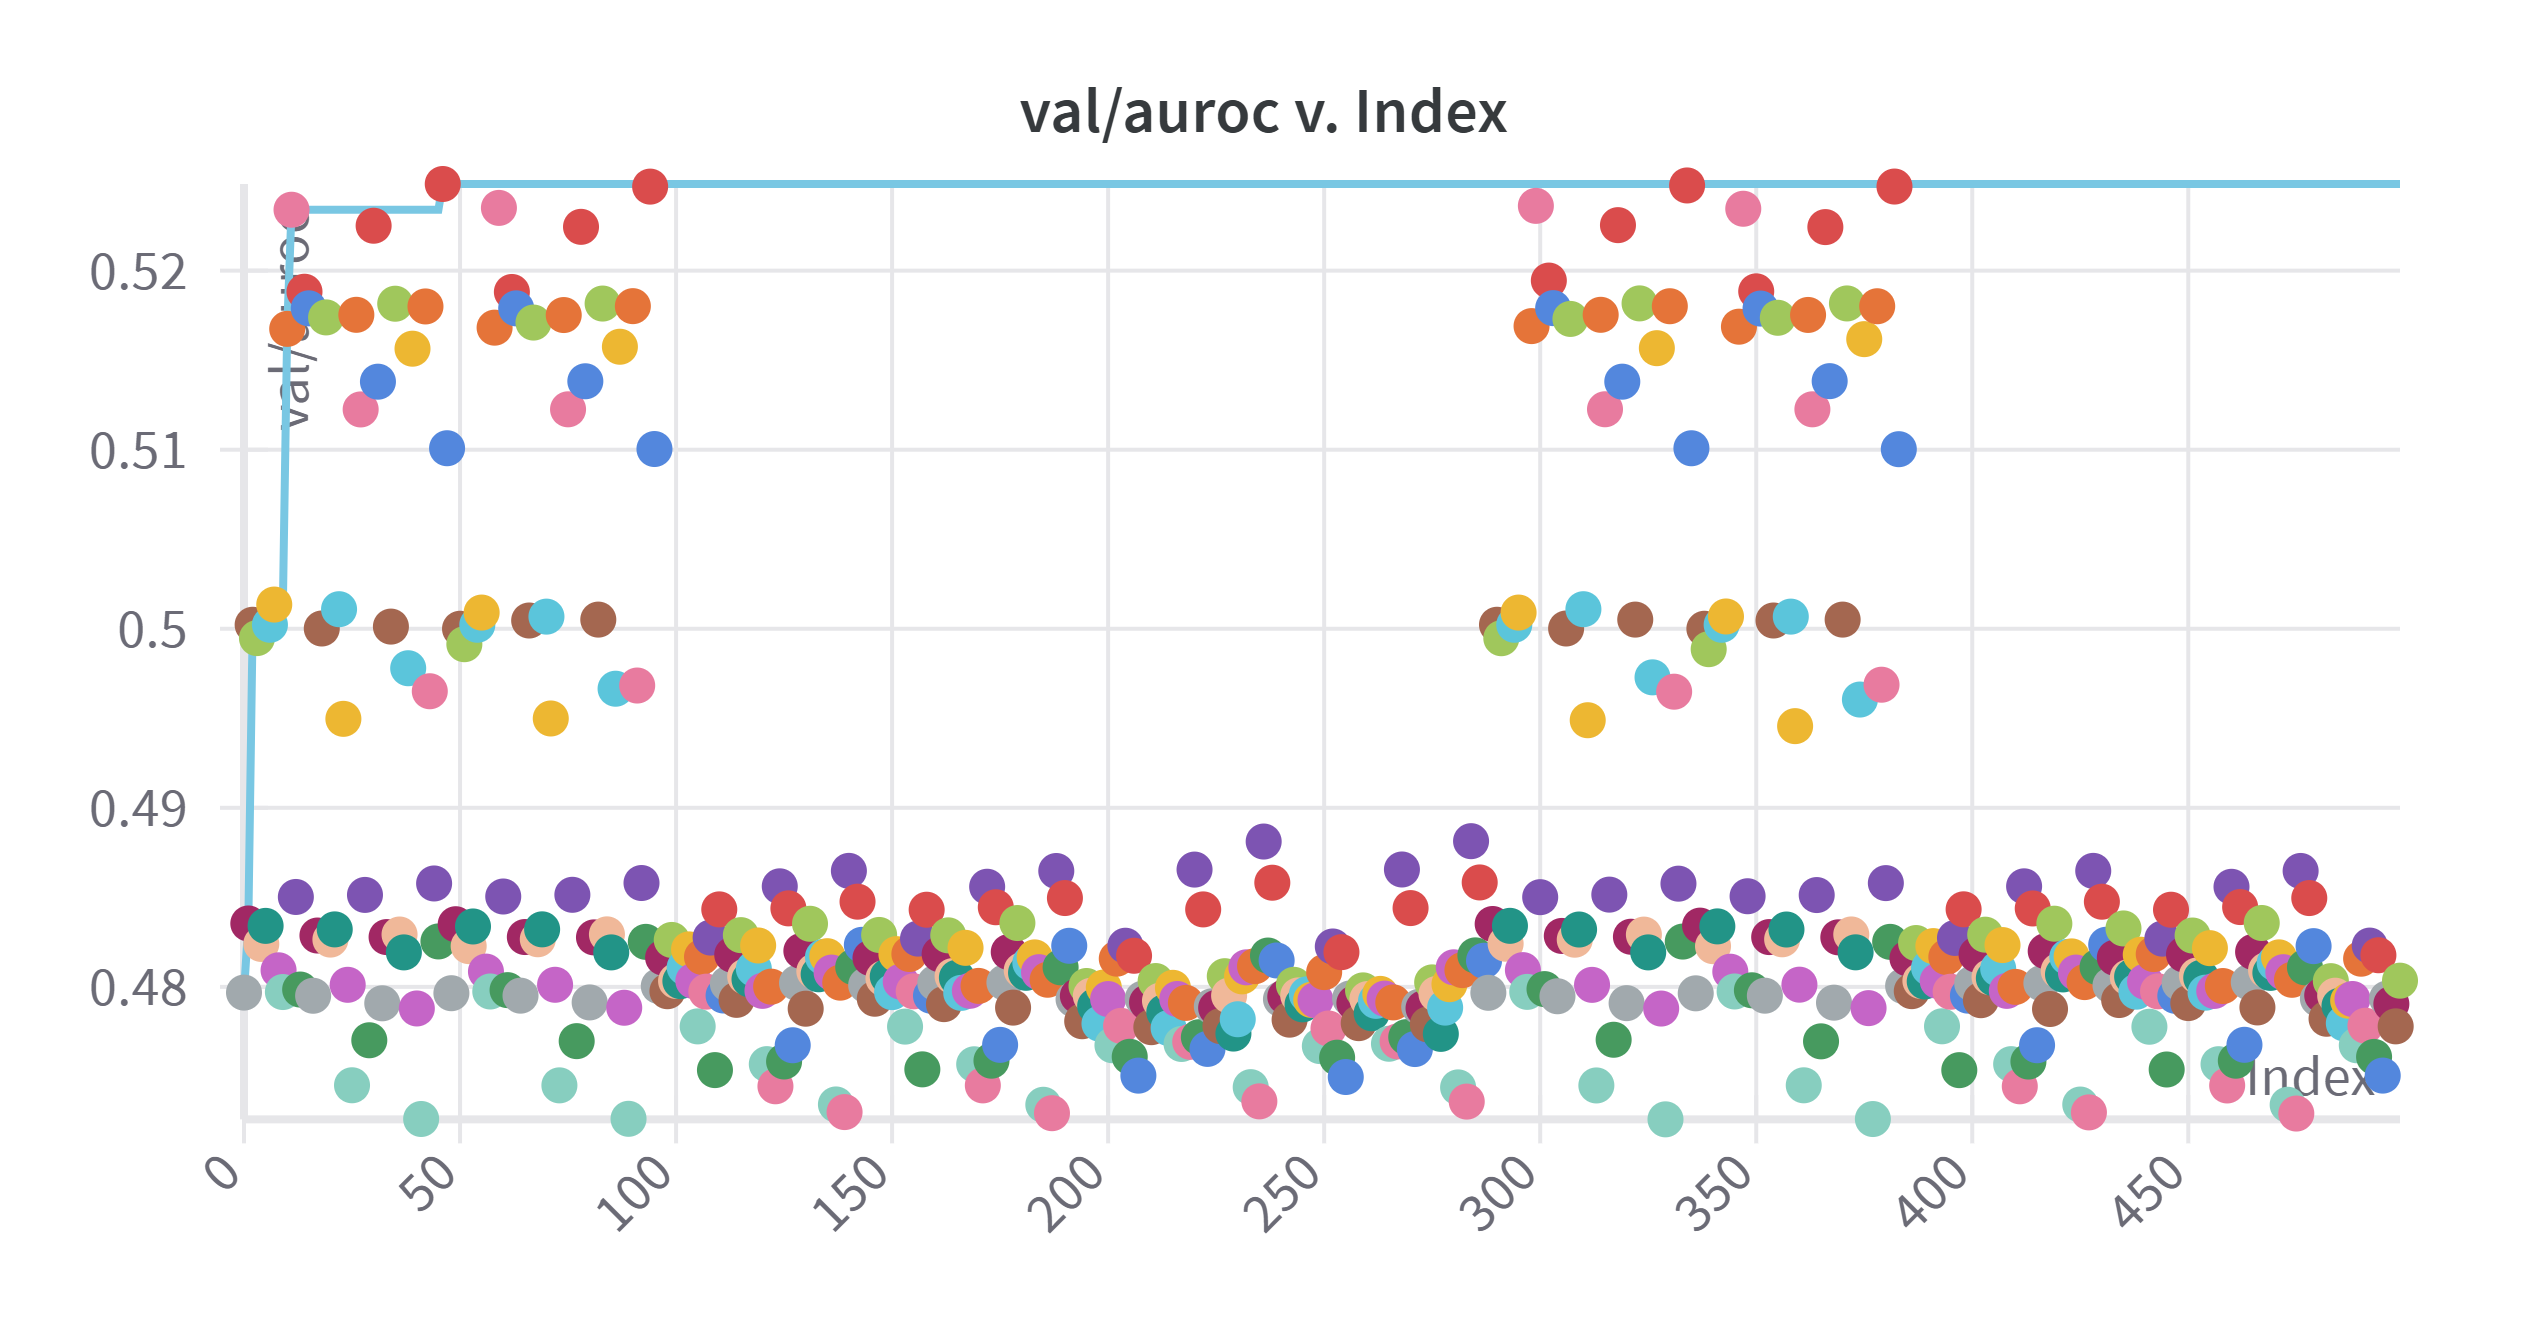
\includegraphics[width=\linewidth]{img/NeuroSAT-soft_sweep.png}
  \caption[Grid search results of soft constraint explainer]{Grid search results of all runs on the soft constraint explainer using WandB \cite{wandb}.}
  \label{fig:soft-sweep}
\end{figure}

\section{Satisfiability of a Hard Constraint Explanation}
\label{sec:sat_expl_hard_cons}
The SAT formula represented by the top-$k$ edges of the validation problem that achieved the highest individual AUROC score for the seed 0 run, with $k$ being the number of edges in its corresponding MUS, is defined as:
\begin{align*}
& (174 \lor 175 \lor 173 \lor 169) \land \\
& (171 \lor 170 \lor 173) \land \\
& (171 \lor 175 \lor 168 \lor 173) \land \\
& (172 \lor 174 \lor 171) \land \\
& (171 \lor 169 \lor 168 \lor 174) \land \\
& (\neg 170) \land \\
& (170 \lor 173 \lor 168) \land \\
& (\neg 168 \lor 171) \land \\
& (172 \lor \neg 168 \lor \neg 170) \land \\
& (169 \lor 171 \lor 172 \lor \neg 174) \land \\
& (175 \lor 173 \lor 168)
\end{align*}
We note that this subset of clauses is satisfiable and therefore not an unsatisfiable core. It is important to note that setting $k$ as the number of edges in its corresponding MUS only makes sense if the MUS is known to be the \ac{GT}. Since we do not know this, this selection of $k$ can be seen as arbitrary. However, a selection is necessary in the context of PGExplainer, since a dynamic way of getting the most important explanation edges was not provided in the original.

    \cleardoublepage
    \phantomsection
    \addcontentsline{toc}{chapter}{Affidavit}
    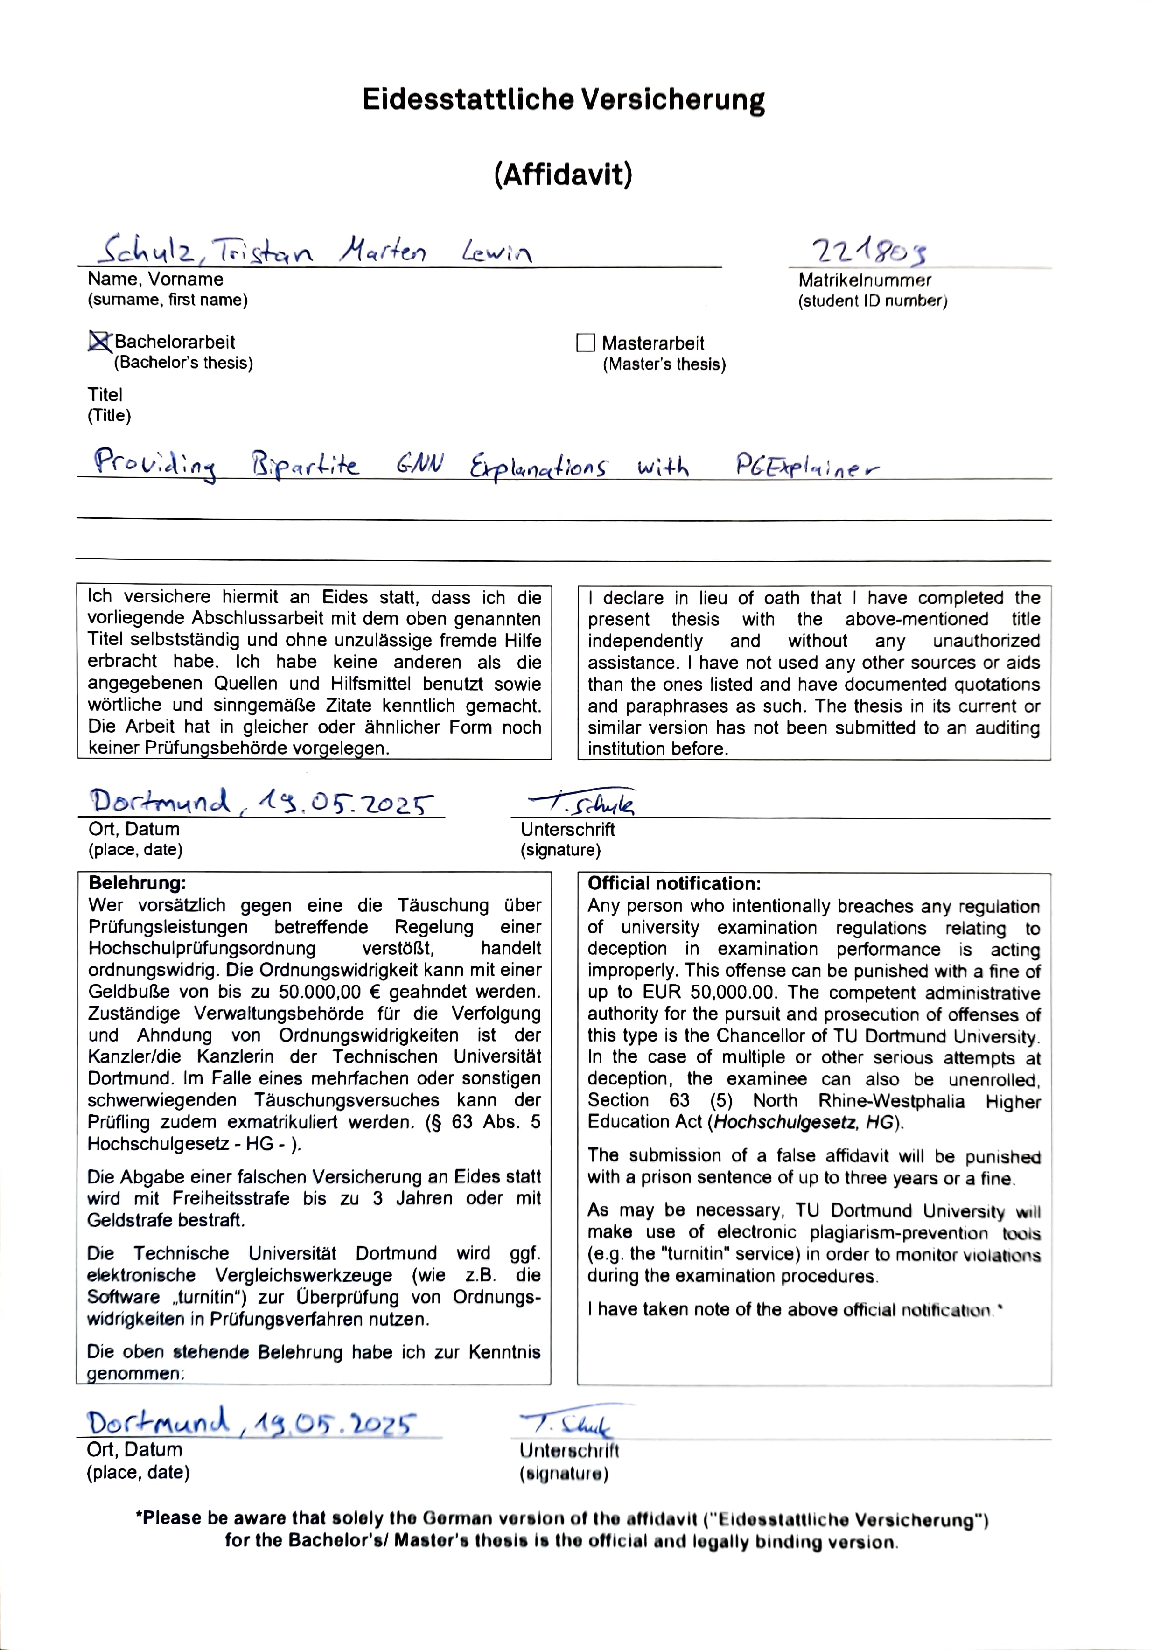
\includepdf[pages=-]{Eidesstattliche_Versicherung_Signed}
\end{document}